\documentclass[11pt,a4paper]{report}

\usepackage{a4}
\usepackage{latexsym}
\usepackage[latin1]{inputenc}
\usepackage{pstricks, pst-node, pst-tree}
\usepackage{listings}
\usepackage{graphics}
\usepackage{wrapfig}

\lstset{language=[95]Ada}

\linespread{1.1}

\title{Ada Crypto Library (ACL) aka libadacrypt-dev\\ Documentation v. 0.1.0 }
\author{Christian Forler}
\date{\today}

%Hyphenation
\hyphenation{dev Gathering Ciphertext Message libacl Byte Word DWord Arrays}
\hyphenation{Crypto Ferguson Initial Private}

\begin{document}

\maketitle
\tableofcontents

  \chapter{Introduction}
The Ada Crypto Library (ACL) is a free cryptographic library for Ada.
One of the two main design objectives of this library was to create
an \textbf{intuitive and clean API}. The other goal was to use a clean
programming style in order to actively support and simplify formal code
verification. Due to this, the ACL has been coded without the
following 'features':
\begin{itemize}
\item access types (pointers)
\item inline assembler
\item tagged types (objects)
\item goto statements
\end{itemize}

Goto statements and access types have been avoided as they make the
source more complex and might cause problems during formal verification
of the code. No tagged types have been used as procedures and methods may
be overwritten and the actual method that is being utilised is determined
during runtime (dynamic dispatching). This results in massive problems during
formal code verification. Inline assembler has been avoided cause it involves
a very unclean programming style and can be used for omitting the strict typing
of ADA. Due to this restrictions, the actual code quality increases with
respect to verification and security, however they also lead to decreased
performance. 
If you favor performance over clean design, you should possibly look for
anothercryptographic library. Unfortunately, there are currently no other free 
cryptographic libraries for ADA I can refer to.\\
The ACL has the status of a draft. Neither a formal code review nor a code 
audit have been performed. At the time of writing, the author of the ACL is the
only one who has dealt with the implementation's details.
For instance, there might be the possibility that sensible material, such as 
the key, might still be resident within the RAM after a program using the ACL 
has been terminated. A storage pool dealing with this restriction is currently 
being developed. Most of the other cryptographic libraries that share this 
limitation do not inform about the possible weakness. Those libraries should 
not be used as they can not be considered reliable.\\
The following paragraph subsumes the disadvantages of the ACL I know:
\begin{itemize}
\item missing cleanup of stack and heap
\item no big endian support
\item bad performance
\end{itemize}
This documentation subsumes the installation and the topological structure.
Afterwards, it solely describes the API. Each package and it's API are 
introduced within a separate chapter. Each chapter concludes with an example.\\
If you should have any questions about the ACL, encounter a bug or want to 
contribute one or several packages, feel free to contact me via email at: 
crypto@shortie.inka.de.\\

\subsection{TODO List}
\begin{itemize}
\item optimisation
\item own storage pool
\item extension (Tiger2, RSA-PSS, Poly1305-AES etc.)  
\end{itemize}

%%%%%%%%%%%%%%%%%%%%%%%%%%%%%%%%%%%%%%%%%%%%%%%%%%%%%%%%%%%%%%%%%%%%%%%%%%%

\section{Installation HOWTO}
\subsection{libadacrpyt-dev}
On a Linux system, the following packages are required for installing the ACL:
\begin{itemize}
\item tar 
\item gnat 
\item make
\item bunzip2 
\item binutils
\end{itemize}

\subsubsection{Compilation}
The following commands can be used for decompressing and compiling the ACL as 
well as the regression test included.
\begin{itemize}
\item \texttt{tar cjf acl.tar.bz2}
\item \texttt{cd crypto}
\item \texttt{make}
\item \texttt{make acltest}
\end{itemize}

\subsubsection{Testing}
Before you actually install the ACL you should run the regression test in
order to make sure the ACL properly works on your computer system. The
regression test approximately takes 30 seconds on a PII 450. The following
command sequence can be used for running the regression test.\\

\begin{itemize}
\item \texttt{cd test}
\item \texttt{./acltest}
\item \texttt{cd ..}
\end{itemize}

\subsubsection{Installation}
If no errors were encountered during the regression test, the ACL can
be installed by issuing the following command:\\
\hspace*{1cm} \texttt{su -c ``make install''}\ \\

\subsubsection{De-installation}
The following command can be used for removing the ACL: \\
\hspace*{1cm} \texttt{su -c ``make uninstall''}\ \\

\subsubsection{Recompilation}
The following commands can be used for recompiling the ACL:\\
\begin{itemize}
\item \texttt{make clean acltest\_clean}
\item \texttt{make}
\item \texttt{make acltest}
\end{itemize}


\subsection{libadacrypt}
\subsubsection{Installiation}
\subsubsection{Shared Library}
The ACL may be installed as a shared library (libacl.so) with the following 
commands:
\begin{itemize}
\item \texttt{make shared}
\item \texttt{make install-shared}
\end{itemize}

\subsubsection{De-installation}
The shared library can be de-installed with the following command:\\
\hspace*{1cm} \texttt{su -c ``make uninstall-shared''}\ \\


\subsection{Documentation}
The tetex-bin (latex) and the tetex-extra packages are needed to install this 
documentation The complete ACL documentation (german \& english) can be 
generated with  the following command:\\
\hspace*{1cm} \texttt{make doc}\ \\ 
\ \\
The documentation will be copied to  
\texttt{/usr/local/share/doc/libadacrypt-dev} with the following command:
\hspace*{1cm} \texttt{su -c ``make install-doc''}\\ 
\ \\
The documentation in \texttt{/usr/local/share/doc/libadacrypt-dev} can be
uninstalled with the following command:
\hspace*{1cm} \texttt{su -c ``make uninstall-doc''}\\ 
\ \\
The documentation can be departed with the following command:
\hspace*{1cm} \texttt{su -c ``make uninstall-doc''}\\



\subsubsection{Adaptations}
The Makefiles can be found in the \texttt{src} directory. It can be used for
adapting the following variables:
\begin{itemize}
\item LIBDIR : installation path for the shared library.
\item INSTDIR : installation path for the ACL.
\end{itemize}
Besides the installation path for the documentation also be changed. Thereto
the variable \texttt{DOCPATH} in \texttt{doc/en/Makefile} and
\texttt{doc/de/Makefile} must be changed.


%%%%%%%%%%%%%%%%%%%%%%%%%%%%%%%%%%%%%%%%%%%%%%%%%%%%%%%%%%%%%%%%%%%%%%%%%%%

\section{Layout of Directories and Packages}
\subsection{Directories}
\begin{itemize}
\item doc : documentation
\item ref : references and specifications
\item src : source code
\item test : regression test
\end{itemize}

%%%%%%%%%%%%%%%%%%%%%%%%%%%%%%%%%%%%%%%%%%%%%%%%%%%%%%%%%%%%%%%%%%%%%%%%%%%

\subsection{Package Layout}
The Ada Crypto Library (ACL) subsumes the following packages (components).
\begin{description}
\item[Crypto:]\ \\ 
  This is the root package of the ACL.
  All other ACL packages start with the \textit{Crypto} prefix.
\item[Crypto.Types:] \ \\
  The fundamental types of the ACL (such as Byte) and their corresponding basic
  functionality are located within this package.
  Utilisation of the ACL is very limited without including this package.  
\item[Crypto.Random:] \ \\
  This package implements an interface between an external random bit generator
  an the ACL.
\item[Crypto.Symmetric:]\ \\
  This is the root package for the symmetric branch.
\item[Crypto.Symmetric.Algorithm:]\ \\
  This branch of the ACL tree contains the symmetric algorithms for the
  blockciphers and the hashfunctions.\\
\item[Crypto.Symmetric.Algorithm.Oneway:]\ \\
  Each algorithm has an oneway algorithm. Symmetric oneway algorithms are
  symmetric algorithms that only work in one direction, and can
  either be used for en- or decryption of data.
\item[Crypto.Symmetric.Blockcipher:]\ \\
  This generic package can be used for generating a block cipher out of
  a symmetric algorithm.
\item[Crypto.Symmetric.Oneway\_Blockcipher:]\ \\
  This package can be used for generating a oneway block cipher out of a
  symmetric oneway algorithm.
\item[Crypto.Symmetric.MAC:]
  This is the root package of the mac branch.
\item[Crypto.Symmetric.Mode:]\ \\
  This branch subsumes multiple modes of operation for block ciphers.
\item[Crypto.Symmetric.Mode.Oneway:]\ \\
  This branch subsumes multiple modes of operation for oneway block ciphers.
\item[Crypto.Asymmetric:]\ \\
  This is the root package of the asymmetric branch.
\item[Crypto.Asymmetric.DSA:]\ \\
  This package can be used for generating and verifying digital signatures.
\item[Crypto.Asymmetric.RSA:]\ \\
  This package can be used for asymmetric en- and decryption of data.
\end{description}


\begin{figure}
  \scalebox{0.90}{%
  \pstree[nodesep=2pt]{\TR{Crypto}}{%
    \pstree{\TR{Types}}{%
      \TR{Big\_Numbers}}
    \TR{Hashfunction}
    \pstree{\TR{Symmetric}}{%
      \pstree{\TR{Algorithm}}{%
	\Tr{Oneway}}
      \TR{Blockcipher} 
      \TR{MAC}
      \TR{Oneway\_Blockcipher}
      \pstree{\TR{Mode}}{%
	\TR{Oneway}}} % end symmetric
    \TR{Random} 
    \pstree{\TR{Asymmetric}}{%
      \TR{DSA} \TR{RSA}}
}}
\end{figure}
    

  \chapter{Crypto}

Crypto is an empty root package. This package does not contain any code.
It's sole purpose is to provide an unique namespace for all ACL packages.
As all packages are descendants of this package, their names start with
the prefix Crypto (e.g. Crypto.Foo.Bar).


 

  \chapter{Crypto.Types}

This package provides the fundamental types of the ACL and their base 
functions.\\ 
\ \\
{\large \textbf{IMPORTANT:} \\
  When using the ACL you should in any case import this package via
  \begin{lstlisting}{}
    with Crypto.Types;
  \end{lstlisting}
  }

%%%%%%%%%%%%%%%%%%%%%%%%%%%%%%%%%%%%%%%%%%%%%%%%%%%%%%%%%%%%%%%%%%%%%%%%%%%
%%%%%%%%%%%%%%%%%%%%%%%%%%%%%%%%%%%%%%%%%%%%%%%%%%%%%%%%%%%%%%%%%%%%%%%%%%%
%%%%%%%%%%%%%%%%%%%%%%%%%%%%%%%%%%%%%%%%%%%%%%%%%%%%%%%%%%%%%%%%%%%%%%%%%%%

\section{Fundamental Types}
The fundamental respective primary types are exclusively modular types,
this means that an overflow or underrun of a variable does not lead to an
exception. If the result of an operation is not within the scope of a modular
type, $n:=2**Type'Size=Type'Last+1$ will be added to or subtracted for it
until the result is within the scope of the modular type. \\

\begin{lstlisting}{}
type Bit is mod 2 ** 1;
for Bit'Size use 1;

type Byte is mod 2 ** 8;
for Byte'Size use  8;

type Word is mod 2 ** 32;
for Word'Size use 32;

type DWord is mod 2 ** 64;
for DWord'Size use 64;
\end{lstlisting}

%%%%%%%%%%%%%%%%%%%%%%%%%%%%%%%%%%%%%%%%%%%%%%%%%%%%%%%%%%%%%%%%%%%%%%%%%%%
%%%%%%%%%%%%%%%%%%%%%%%%%%%%%%%%%%%%%%%%%%%%%%%%%%%%%%%%%%%%%%%%%%%%%%%%%%%


\subsubsection{Example}
\begin{lstlisting}[frame=brtl]{Modular Type}
with Ada.Text_IO;
with Crypto.Types;
procedure Example is
   use Crypto.Types;
   -- Byte has a scope of 0..255
   A, B : Byte;
begin
   A := 100;
   B := A + 250; -- Overflow at B
   A := A - 250; -- Underrun at A
   Ada.Text_IO.Put_Line("A: " &  A'IMG);
   Ada.Text_IO.Put_Line("B: " &  B'IMG);
end example;
\end{lstlisting}
\textit{Program output:\\}
\texttt{A:  106\\B:  94}

%%%%%%%%%%%%%%%%%%%%%%%%%%%%%%%%%%%%%%%%%%%%%%%%%%%%%%%%%%%%%%%%%%%%%%%%%%%
%%%%%%%%%%%%%%%%%%%%%%%%%%%%%%%%%%%%%%%%%%%%%%%%%%%%%%%%%%%%%%%%%%%%%%%%%%%
%%%%%%%%%%%%%%%%%%%%%%%%%%%%%%%%%%%%%%%%%%%%%%%%%%%%%%%%%%%%%%%%%%%%%%%%%%%


\subsection{Derived Types}
Derived types are types that are derived from elementary types. Regularly,
these are arrays, consisting of elementary types. \textbf{All non-private
arrays consisting of elementary types are interpreted as n-bit numbers within
the ACL}, where the first element (First) is considered to be the 
most-significant and the last element (Last) the least-significant element of 
the number. This is a fundamental characteristic of the ACL.

\begin{tabular}{p{\textwidth}}
\subsubsection{Bit}
\begin{lstlisting}{Bits}
  type Bits is array (Integer range <>) of Bit;
\end{lstlisting}\ \\ \ \\
\hline 
\end{tabular}


\begin{tabular}{p{\textwidth}}
\subsubsection{Bytes} 
\begin{lstlisting}{Bytes}
  type Bytes is array (Integer range <>) of Byte;
  
  subtype Byte_Word  is Bytes (0 .. 3);
  subtype Byte_DWord is Bytes (0 .. 7);

  subtype B_Block32  is Bytes (0 ..  3);
  subtype B_Block48  is Bytes (0 ..  5);
  subtype B_Block56  is Bytes (0 ..  6);
  subtype B_Block64  is Bytes (0 ..  7);
  subtype B_Block128 is Bytes (0 .. 15);
  subtype B_Block160 is Bytes (0 .. 19); 
  subtype B_Block192 is Bytes (0 .. 23);
  subtype B_Block256 is Bytes (0 .. 31);
\end{lstlisting}
A B\_BlockN always consists of a N bit array separated into N/8 Bytes.
The subtype B\_Block256 for example is a 256-bitstring, separated into
32 (258/8) byte blocks. In Ada, it can be represented by a byte array
consisting of 32 elements. \\ \ \\
\hline
\end{tabular}

%%%%%%%%%%%%%%%%%%%%%%%%%%%%%%%%%%%%%%%%%%%%%%%%%%%%%%%%%%%%%%%%%%%%%%%%%%%

\begin{tabular}{p{\textwidth}}
  \subsubsection{Words} 
  \begin{lstlisting}{Words}
  type Words   is array (Integer range <>) of Word;
  
  subtype W_Block128  is Words(0 .. 3);
  subtype W_Block160  is Words(0 .. 4);
  subtype W_Block192  is Words(0 .. 5);
  subtype W_Block256  is Words(0 .. 7);
  subtype W_Block512  is Words(0 .. 15);
  \end{lstlisting}
  A W\_BlockN always consists of a N bit array separated into N/32 Words.
  The subtype W\_Block256 for example is a 256-bitstring, separated into 8 (256/32) Word
  elements. In Ada, it can be represented by a Word array consisting of 8 elements.\\ \ \\
\hline
\end{tabular}

%%%%%%%%%%%%%%%%%%%%%%%%%%%%%%%%%%%%%%%%%%%%%%%%%%%%%%%%%%%%%%%%%%%%%%%%%%%
  
\begin{tabular}{p{\textwidth}}
  \subsubsection{DWords} 
  \begin{lstlisting}{DWords}
  type DWords   is array (Integer range <>) of DWord  
    
  subtype DW_Block256   is DWords(0 ..  3);
  subtype DW_Block384   is DWords(0 ..  5);
  subtype DW_Block512   is DWords(0 ..  7);
  subtype DW_Block1024  is DWords(0 .. 15);
  \end{lstlisting}
  A DW\_BlockN always consists of a N bit array separated into N/64 Words.
  The subtype DW\_Block256 for example is a 256-bitstring separated into 4 
  (256/64) DWord
  elements. In Ada, it can be represented by a DWord array with 4 elements.\\ 
\ \\
\hline
\end{tabular}

%%%%%%%%%%%%%%%%%%%%%%%%%%%%%%%%%%%%%%%%%%%%%%%%%%%%%%%%%%%%%%%%%%%%%%%%%%%
  
\begin{tabular}{p{\textwidth}}
  \subsubsection{Strings} 
  \begin{lstlisting}{Strings}
    subtype Hex_Byte  is String (1.. 2);
    subtype Hex_Word  is String (1.. 8);
    subtype Hex_DWord is String( 1..16);
  \end{lstlisting}\ \\
  \hline
\end{tabular}

%%%%%%%%%%%%%%%%%%%%%%%%%%%%%%%%%%%%%%%%%%%%%%%%%%%%%%%%%%%%%%%%%%%%%%%%%%%

\begin{tabular}{p{\textwidth}}
\subsubsection{Message blocks} 
\begin{lstlisting}{Message blocks}
subtype Message_Block_Length512  is Natural range 0 ..  63;
subtype Message_Block_Length1024 is Natural range 0 .. 127;

\end{lstlisting}
The Message\_Block\_Length types indicate the length of the actual message
stored within a 512 or 1024 bit message block M in characters (Bytes).
For example, splitting a 1152 bit message into 512 bit blocks results in
three 512 bit blocks. The actual message length of the last block is 16 
($1280 - 2 \cdot 512 = 128 / 8 = 16$).
The remaining 384 bits of the last message block are ''empty'', 
this means that they do not contain any part of the original message.
A variable of type M\_Length512 would be set to 32 in this case.
As seen above, these variable types are used for message block padding.
More information about padding can be found in the chapter about hash
functions (\ref{hash}).\\ \ \\
\hline 
\end{tabular}\ \\

%%%%%%%%%%%%%%%%%%%%%%%%%%%%%%%%%%%%%%%%%%%%%%%%%%%%%%%%%%%%%%%%%%%%%%%%%%%
%%%%%%%%%%%%%%%%%%%%%%%%%%%%%%%%%%%%%%%%%%%%%%%%%%%%%%%%%%%%%%%%%%%%%%%%%%%

\subsection{Bit-shifting Functions}
\begin{lstlisting}{Types-functions}
     function Shift_Left   (Value  : Byte;
                          Amount : Natural) 
			  return Byte;

   function Shift_Right  (Value  : Byte;
                          Amount : Natural) 
			  return Byte;

   function Rotate_Left  (Value  : Byte;
                          Amount : Natural)
			  return Byte;

   function Rotate_Right (Value  : Byte;
                          Amount : Natural)
			  return Byte;


   function Shift_Left   (Value : Word;
                          Amount : Natural) 
                          return Word;

   function Shift_Right  (Value  : Word; 
                          Amount : Natural) 
			  return Word;

   function Rotate_Left  (Value  : Word; 
                          Amount : Natural) 
			  return Word;

   function Rotate_Right (Value  : Word; 
                          Amount : Natural) 
			  return Word;


   function Shift_Left   (Value  : DWord; 
                          Amount : Natural) 
			  return DWord;

   function Shift_Right  (Value  : DWord;
                          Amount : Natural)
			  return DWord;

   function Rotate_Left  (Value  : DWord; 
                          Amount : Natural)
                           return DWord;

   function Rotate_Right (Value  : DWord;
                          Amount : Natural) 
			  return DWord;
\end{lstlisting}\ \\

%%%%%%%%%%%%%%%%%%%%%%%%%%%%%%%%%%%%%%%%%%%%%%%%%%%%%%%%%%%%%%%%%%%%%%%%%%%
%%%%%%%%%%%%%%%%%%%%%%%%%%%%%%%%%%%%%%%%%%%%%%%%%%%%%%%%%%%%%%%%%%%%%%%%%%%

\subsection{Basic Functions}\ 

\begin{tabular}{p{\textwidth}}
  \textbf{XOR}\ \\
  \begin{lstlisting}{}
    function "xor" (Left, Right : Bytes)   return Bytes;
    function "xor" (Left, Right : Words)   return Words;
    function "xor" (Left, Right : DWords) return DWords;
  \end{lstlisting}
  \underline{Prerequisite:}\\ Left'Length = Right'Length\\
  \underline{Exception:}\\
  Prerequisite violation :  Constraint\_Byte/Word/DWord\_Error\\ \ \\
  This functions perform a field-wise concatenation of the first two input 
  fields by
  using the XOR operation. Left(Left'First) is XOR concatenated with
  Right(Right'First) and Left(Left'Last) with Right(Right'Last).\\ \ \\
  \hline\\
\end{tabular}

%%%%%%%%%%%%%%%%%%%%%%%%%%%%%%%%%%%%%%%%%%%%%%%%%%%%%%%%%%%%%%%%%%%%%%%%%%%

\begin{tabular}{p{\textwidth}}
 \textbf{+}\ \\
\begin{lstlisting}{}
  function "+" (Left : Bytes; Right  : Byte)     return Bytes;
  function "+" (Left : Byte; Right   : Bytes)    return Bytes;
  function "+" (Left : Words; Right  : Word)     return Words;
  function "+" (Left : Word; Right   : Words)    return Words;
  function "+" (Left : Words; Right  : Byte)     return Words;
  function "+" (Left : DWords; Right : DWord)  return DWords;
  function "+" (Left : DWord;  Right : DWords) return DWords;
  function "+" (Left : DWords; Right : Byte)     return DWords;
\end{lstlisting}
\end{tabular}

\begin{tabular}{p{\textwidth}}
  This function interprets Left and Right as numbers where Left(Left'First)
  and Right(Right'First) denotes the least significant Byte/Word/DWord and
  Left(Left'Last) and Right(Right'Last) denotes the most significant
  Byte/Word/DWord of a number.
  The result of this function is the sum of the two numbers. \\ \ \\
  \textbf{Example:}
\begin{lstlisting}{}
procedure plus is 
  A : Byte := 200;
  B : Bytes(0..1) := (0 => 100, 1 => 16); 
  begin
  B := A+B; -- B := 2#11001000#+2#10000_01100100# 
  -- B(0) = 2#101100# = 44
  -- B(1) = 2#010001# = 17
end plus;
\end{lstlisting}
\end{tabular}

%%%%%%%%%%%%%%%%%%%%%%%%%%%%%%%%%%%%%%%%%%%%%%%%%%%%%%%%%%%%%%%%%%%%%%%%%%%
%%%%%%%%%%%%%%%%%%%%%%%%%%%%%%%%%%%%%%%%%%%%%%%%%%%%%%%%%%%%%%%%%%%%%%%%%%%

\subsection{Transformation Functions}\ \\

\subsubsection{ByteN}
\begin{lstlisting}{}
  function Byte0 (W : Word)  return Byte;
  function Byte1 (W : Word)  return Byte;
  function Byte2 (W : Word)  return Byte;
  function Byte3 (W : Word)  return Byte; 

  function Byte0 (D : DWord) return Byte;
  function Byte1 (D : DWord) return Byte;
  function Byte2 (D : DWord) return Byte;
  function Byte3 (D : DWord) return Byte;
  function Byte4 (D : DWord) return Byte;
  function Byte5 (D : DWord) return Byte;
  function Byte6 (D : DWord) return Byte;
  function Byte7 (D : DWord) return Byte;
\end{lstlisting}
\begin{tabular}{p{\textwidth}}
Let
$\mathtt{W : Word  \equiv B0||B1||B2||B3}$\\
and\\
$\mathtt{D : DWord \equiv B0||B1||B2||B3||B4||B5||B6||B7}$.\\ 
\ \\
Then the first function returns B0 of W,  the second B1 of W and so on.\\ \ \\
\hline\\
\end{tabular}

%%%%%%%%%%%%%%%%%%%%%%%%%%%%%%%%%%%%%%%%%%%%%%%%%%%%%%%%%%%%%%%%%%%%%%%%%%%

\begin{tabular}{p{\textwidth}}   
  \textbf{To\_Bytes}\ \\
  \begin{lstlisting}{}
    function To_Bytes(X : Word)  return Byte_Word;
    function To_Bytes(X : DWord) return Byte_DWord; 

    function To_Bytes(Word_Array  : Words)  return Bytes;
    function To_Bytes(DWord_Array : DWords) return Bytes;

    function To_Bytes(Message : String) return Bytes;
  \end{lstlisting}\\
  The first two functions convert a Word resp. DWord into a Byte\_Word resp.
  a Byte\_DWord.
  The most significant byte of X becomes the first element of the returned
  Byte array und the least significant byte of X becomes the last element of 
  the returned  Byte array.\\ \ \\
  \textbf{Example:}
  \begin{lstlisting}{}
    D : DWord := 16#AA_BB_CC_DD_EE_FF_11_22#;
    B : Byte_DWord := To_Bytes(D);
    -- B(0) := 16#AA#; B(1) := 16#BB#; B(2) := 16#CC#;
    -- B(3) := 16#DD#; B(4) := 16#EE#; B(5) := 16#FF#; 
    -- B(6) := 16#11#; B(7) := 16#22#;
  \end{lstlisting}\\
  The next two functions convert a Word or a DWord array into an Byte array.
  The first element of the input array becomes the first byte of the 
  returned byte array und the least significant byte of the last element 
  becomes the last element of the returned  Byte array.\\ \ \\
  The least function converts an ASCII string in a Byte array.
  For all $I \in$ Message'Range applies:
  B(I) =  Character'Pos(Message(I)).\\  \ \\
\hline\\
\end{tabular}


%%%%%%%%%%%%%%%%%%%%%%%%%%%%%%%%%%%%%%%%%%%%%%%%%%%%%%%%%%%%%%%%%%%%%%%%%%%

\begin{tabular}{p{\textwidth}}
  \textbf{R\_To\_Bytes}\ \\
  \begin{lstlisting}{}
    function R_To_Bytes (X :  Word) return Byte_Word; 
    function R_To_Bytes (X : DWord) return Byte_DWord;
  \end{lstlisting}
  This function transforms a Word resp. DWord into a Byte\_Word
  resp. Byte\_DWord.
  The the most significant Byte of X becomes the first element in the returned
  Byte array and the least  significant Byte of X becomes the last element in 
  the returned Byte array.\\ \ \\
  \hline\\
\end{tabular}

%%%%%%%%%%%%%%%%%%%%%%%%%%%%%%%%%%%%%%%%%%%%%%%%%%%%%%%%%%%%%%%%%%%%%%%%%%%

\begin{tabular}{p{\textwidth}}
  \textbf{To\_Word}\ \\
  \begin{lstlisting}{}
    function To_Word (X : Byte_Word)  return Word;

    function To_Word (A,B,C,D : Byte) return Word;

    function To_Word (A,B,C,D : Character) return Word;  
\end{lstlisting}\\ 
  The first function converts a  Byte\_Word into a Word.
  X(Byte\_Word'First) becomes the most significant Byte of the Word,
  X(Byte\_Word'Last) the last significant one.\\ \ \\
  The next function  transforms four Bytes (A, B, C, D) into a Word.
  A becomes the most significant Byte of the Word, D the last significant one.
  \\ \ \\
  The least function transforms four Characters (A, B, C, D) into a Word.
  The first Character (A'Pos) becomes the most significant byte of the
  resulting Word, the last character (D'Pos) the least significant one.\ \ \\
  \hline\\
\end{tabular}

%%%%%%%%%%%%%%%%%%%%%%%%%%%%%%%%%%%%%%%%%%%%%%%%%%%%%%%%%%%%%%%%%%%%%%%%%%%

\begin{tabular}{p{\textwidth}}   
  \textbf{R\_To\_Word}\ \\
  \begin{lstlisting}{}
    function R_To_Word (X : Byte_Word) return Word;   
  \end{lstlisting}
  This function transform a Byte\_Word into a Word.
  X(Byte\_Word'First) becomes the least significant Byte of the Word,
  X(Byte\_Word'Last) becomes the most significant Byte of the one.\\ \ \\
  \hline\\
\end{tabular}

%%%%%%%%%%%%%%%%%%%%%%%%%%%%%%%%%%%%%%%%%%%%%%%%%%%%%%%%%%%%%%%%%%%%%%%%%%%


\begin{tabular}{p{\textwidth}}
  \textbf{To\_Words}\ \\
  \begin{lstlisting}{}
    function To_Words(Byte_Array : Bytes)  return Words;
  \end{lstlisting}
  This function converts a Byte array into a Word array W
  Byte\_Array(Byte\_Array'First) becomes the most significant byte
  of W'First and the last element the Byte array becomes a byte of W'Last. 
  \textbf{Example:}\\
  \textbf{(i)}
\begin{lstlisting}{}
      B : Bytes(1..6) := (16#0A#, 16#14#, 16#1E#, 
                          16#28#, 16#32#, 16#3C#);
      W : Words := Byte_to_Dwords(B);
      -- W(D'First) = 16#0A_14_1E_28#
      -- W(D'Last)  = 16#32_3C_00_00#
    \end{lstlisting}\\ \ \\
  \textbf{(ii)}\\ \ \\
    \textit{Input:}$B=\underbrace{B(1)||B(2)||B(3)||B(4)}_{W(0)}
    \underbrace{B(5)||B(6)||B(7)||B(8)}_{W(1)}
    \underbrace{B(9)||B(10)}_{W(2)}$\\ \ \\
    \textit{Output:} $W=W(0)||W(1)||W(2)$\\ \ \\
    \hline\\
\end{tabular}

%%%%%%%%%%%%%%%%%%%%%%%%%%%%%%%%%%%%%%%%%%%%%%%%%%%%%%%%%%%%%%%%%%%%%%%%%%%


\begin{tabular}{p{\textwidth}}
  \textbf{To\_DWord}\ \\
  \begin{lstlisting}{} 
    function To_DWord (X : Byte_DWord) return DWord;
  \end{lstlisting}\\
  This function transforms a Byte\_DWord X into a DWord.
  X(Byte\_Word'First) becomes the most significant byte of the DWords,
  X(Byte\_Word'Last) becomes the least significant byte of the one.\\ \ \\
  \hline\\
\end{tabular}

%%%%%%%%%%%%%%%%%%%%%%%%%%%%%%%%%%%%%%%%%%%%%%%%%%%%%%%%%%%%%%%%%%%%%%%%%%%
  
\begin{tabular}{p{\textwidth}}   
\textbf{R\_To\_DWord}\ \\
  \begin{lstlisting}{}
    function R_To_DWord (X : Byte_DWord) return DWord;  
  \end{lstlisting}
  This function transforms a Byte\_DWord X into a DWord.
  X(Byte\_Word'First) becomes the least significant byte of the DWords,
  X(Byte\_Word'Last) becomes the most significant byte of the one.\\ \ \\
  \hline\\
\end{tabular}

%%%%%%%%%%%%%%%%%%%%%%%%%%%%%%%%%%%%%%%%%%%%%%%%%%%%%%%%%%%%%%%%%%%%%%%%%%%

\begin{tabular}{p{\textwidth}}
  \textbf{To\_DWords}\ \\
  \begin{lstlisting}{}
    function To_DWords  (Byte_Array : Bytes) return DWords;
  \end{lstlisting}
  This function transforms a byte array into a DWord array D.
  Byte\_Array(Byte\_Array'First) becomes the most significant byte
  of the D'First and the last element of the Byte array becomes a byte of
  D'Last. \\ \ \\
  \textbf{Example:}
  \begin{lstlisting}{}
    B : Bytes(1..10) : (10, 20, 30, 40, 50, 60, 70, 80, 90, 100);
    D : DWords := Byte_to_Dwords(B);
    -- D(D'First) =             16#0A_14_1E_28_32_3C_46_50#
    -- D(D'Last) = D(First+1) = 16#5A_64_00_00_00_00_00_00#
  \end{lstlisting}\\ \ \\
  \hline\\
\end{tabular}

%%%%%%%%%%%%%%%%%%%%%%%%%%%%%%%%%%%%%%%%%%%%%%%%%%%%%%%%%%%%%%%%%%%%%%%%%%%

\begin{tabular}{p{\textwidth}}
  \textbf{To\_String}\ \\
  \begin{lstlisting}{}
    function Bytes_To_String(ASCII : Bytes) return String;
  \end{lstlisting}
  This function transforms a Byte array into an String. Thereby
  every element of the Byte array will be interpreted as an ASCII-Code.\ \ \\
  \hline\\
\end{tabular}\ \\


%%%%%%%%%%%%%%%%%%%%%%%%%%%%%%%%%%%%%%%%%%%%%%%%%%%%%%%%%%%%%%%%%%%%%%%%%%%

\begin{tabular}{p{\textwidth}}
  \textbf{To\_Hex}\ \\
  \begin{lstlisting}{}
    function To_Hex(B : Byte)  return Hex_Byte;
    function To_Hex(W : Word)  return Hex_Word;
    function To_Hex(D : DWord) return Hex_DWord;
  \end{lstlisting}
  This functions  transforms a Byte, Word or DWord into an 2,8 or 16 byte
  hex string.
  For instance \texttt{Put(To\_Hex(W));} is equivalent to the C code
  \texttt{ printf(``\%08X'', i);}.\\ \ \\
  \textbf{Beispiel:}
\begin{lstlisting}{}
    B : Word := 0;
    W : Word := 16#AABBCCDDEEFF#;
    
    HB:Hex_Byte:=To_Hex(W); -- Es gilt: HB="00".
    HW:Hex_Word:=To_Hex(W); -- Es gilt: HW="0000AABBCCDDEEFF".
  \end{lstlisting}\ \\
\end{tabular}\ \\



%%%%%%%%%%%%%%%%%%%%%%%%%%%%%%%%%%%%%%%%%%%%%%%%%%%%%%%%%%%%%%%%%%%%%%%%%%%

\subsection{Functions}
\begin{lstlisting}{}
   function Is_Zero(Byte_Array  : Bytes)  return Boolean;
   function Is_Zero(Word_Array  : Words)  return Boolean;
   function Is_Zero(DWord_Array : DWords) return Boolean;
\end{lstlisting}
These functions return ``True'' if all fields of the array parameter
contain the value ``0''. Otherwise, ``False'' is returned.\\ \ \\

%%%%%%%%%%%%%%%%%%%%%%%%%%%%%%%%%%%%%%%%%%%%%%%%%%%%%%%%%%%%%%%%%%%%%%%%%%%
%%%%%%%%%%%%%%%%%%%%%%%%%%%%%%%%%%%%%%%%%%%%%%%%%%%%%%%%%%%%%%%%%%%%%%%%%%%

\subsection{Padding Procedures}
 \begin{lstlisting}{}
procedure Padding(Data            : in out Bytes;
                     Message_Length : in  Word;
                     Data2          : out Bytes);

procedure Padding(Data              : in  out Words;
                     Message_Length : in  Word;
                     Data2          : out Words);

 procedure Padding(Data              : in  out DWords;
                      Message_Length : in  Word;
                      Data2          : out DWords); 
 \end{lstlisting}
 \textbf{Parameters:}
 \textit{Data:}\\
 Data has to be an array containing a message.
 The message has to correspond to the following part of Data:\\
 Data(Data'First)..Data(Data'First+(Message\_Length-1))
\textit{Message\_Length:}\\
The length of the message stored in Data.
\textit{Data2:}\\
Is used for some special cases. Regularly
Is\_Zero(Data2) = true after calling this function.\\
\ \\
\textbf{Prerequisites:}
 \begin{enumerate}
 \item Data'Length = Data2'Length
 \item Message\_Length $\le$ Data'Length
 \item Word(Data'Length) - Message\_Length $>$ 2**16-1\footnotemark 
 \end{enumerate}
 \textbf{Postconditions:}
 \begin{enumerate}
 \item Message\_Length $<$ Data'Length-2 $\Rightarrow$ Is\_Zero(Data2) = True
 \item Is\_Zero(Data2) = False  $\Longleftrightarrow$ Message'Length $>$ 
   Data'Length-2
 \end{enumerate}
 \textbf{Exceptions:}\\
 \addtocounter{footnote}{-1} 
\begin{tabular}{l@{ : }l}
 Constraint\_Message\_Length\_Error &  Message\_Length $>$ Data'Length\\
 Constraint\_Length\_Error &  Data'Length $>$ (2 * Byte'Last)
 \footnote{Only if Data is an instance of type Byte}\\
 \end{tabular}\ \\ \ \\
 This functions add a number of null-Bytes/Words/Dwords to a message,
 followed by a Byte/Word/DWord representing the actual number of null-Bytes
 inserted. This might result in the following special cases:
 \begin{enumerate}
 \item Message\_Length+1=Data'Length\\
   After adding a null Byte to the message, no additional space is available
   for appending the actual number of Null-Bytes/Words/DWords inserted to the message
   as Data(Data'Last) has been filled up by the null-Byte/Word/DWord.
   In order to solve this problem, all fields of Data2 except for Data2'Length are set to 0.
   Data2'Last is set to Data2'Length.
 \item Message\_Length=Data'Length\\
   This case is treated analogous to the first special case with the following deviations:
   \begin{enumerate}
   \item No null-Byte/Word/DWord is appended to the message
   \item Data2'Last := Data2'Length-1
   \end{enumerate}
 \end{enumerate}

\subsubsection{Example}
\begin{lstlisting}{}
... 
  package BIO is new Ada.Text_Io.Modular_IO (Byte);

  X : Bytes(1..9) := (1 => 2, 2 => 4, 3 => 6, 
                      4 => 8, 5 => 9, others =>1);
  Y : Bytes(1..9);
begin
  Padding(X, N, Y);
  Put("X:");
  for I in X'Range loop
     Bio.Put(X(I));
  end loop;
  New_Line;
  if Is_Zero(Y) = False  then
      Put("Y:");
      for I in Y.all'Range loop
	 Bio.Put(Y.all(I));
      end loop;
   end if;
...
\end{lstlisting}\ \\
\underline{Output:}\\
\begin{itemize}
\item N = 5\\
  X : 2   4   6  8  9   0   0   0   3
\item N = 8\\
  X : 2   4   6   8   9   1   1   1   0\\
  Y : 0   0   0   0   0   0   0   0   9
\item N = 9\\
  X : 2   4   6   8   9   1   1   1   1\\
  Y : 0   0   0   0   0   0   0   0   8
\end{itemize}





  \chapter{Crypto.Random}
\section{Einf�hrung}
Dieses Paket greift defaultm��ig auf ``dev/random/'' zu.
Unter Linux ist \\``/dev/random'' ein Pseudodevice das kryptographisch sichere
Pseudozufallsbits liefert. Wenn sie ein Betriebsystem verwenden das kein 
solches Pseudodevice besitzt, dann k�nnen sie dies mit Hilfe von mit 
Brian Warners ``Entropy Gathering Daemon''(EGD), der unter
\textit{http://www.lothar.com/tech/crypto/} zu finden 
ist,  nachinstallieren. Der EGD ist ein Userspace-Implementierung des 
Linux-Kernel-Devices ``dev/random/'', das kryptograpisch sichere
Zuallsbits generiert.\\
Im privaten Teil befindet sich die Variable ``Path''. Diese Variable gibt den
Pfad zu einer Datei, Named Pipe oder Ger�t das krytograpisch sichere
Zufallsbits enth�lt an.  Dadurch sind Sie in der Lage die ACL auch an eine
kryptograpisch sichere (Pseudo-)Zufallsbitquelle eines nicht POSIX kompatiblen
Betriebsystems wie Windows XP anbinden.\\
Weiterhin besteht die M�glichkeit unter Windows den Marsaglia- RNG zu benutzen.
Er ist ein lagged- Fibonacci Sequenz Generator und erzeugt 24-Bit real numbers
im Intervall [0,1].\\
Eigenschaften: Kombination zweier unterschiedlicher Generatoren, welche fort-
laufende Bits erzeugen. Diese werden durch zwei weitere Generatoren zu einer 
Tabelle Kombiniert.
Die Prozedur ''Start'' initialisiert diese Tabelle, welche von der Funktion 
''Next'' genutzt wird um die n�chste Zufallszahl zu generieren.

\section{API}
\subsection{Prozeduren}
\begin{tabular}{p{\textwidth}}
  \begin{lstlisting}{}
    procedure Read(B : out Byte);
    procedure Read(W : out Word);
    procedure Read(D : out DWord);
  \end{lstlisting}
  Bei diesen drei Prozeduren wird B, W oder D mit Bits aus der
  verwendeten Pseudozufallsbit-Quelle gef�llt.\\ \ \\
  \hline\\
\end{tabular}

\begin{tabular}{p{\textwidth}}
  \begin{lstlisting}{}
    procedure Read(Byte_Array  : out Bytes);
    procedure Read(Word_Array  : out Words);
    procedure Read(DWord_Array : out DWords);
  \end{lstlisting}\\
  Diese drei Prozeduren wirden die �bergebenen Arrays mit Bits aus der 
  verwendeten Pseudozufallsbit-Quelle gef�llt. \\ \ \\
\end{tabular}

\begin{tabular}{p{\textwidth}}
  \begin{lstlisting}{}
    procedure Start(
    New_I : Seed_Range_1 := Default_I;
    New_J : Seed_Range_1 := Default_J;
    New_K : Seed_Range_1 := Default_K;
    New_L : Seed_Range_2 := Default_L);
  \end{lstlisting}\\
  \\ \ \\
\end{tabular}

\subsection{Exceptions}
\begin{tabular}{p{\textwidth}}
  \begin{lstlisting}{}
    Random_Source_Does_Not_Exist_Error : exception;
  \end{lstlisting}\\
  Diese Ausnahme wird aufgerufen, wenn kein (kryptograpisch sicherer) 
  Pseudozufallsbit-Quelle gefunden wurde.\\ \ \\
  \hline\\
  \begin{lstlisting}{}
    Random_Source_Read_Error : exception;
  \end{lstlisting}\\
  Wenn ein Lesefehler bei einem Zugriff auf die Pseudozufallsbit-Quelle 
  auftritt, wird die folgende Aufnahme ausgeworfen. \\ \ \\
  \hline\\
\end{tabular}

\begin{lstlisting}{}
\end{lstlisting}

  \part{Advanced}
\chapter{Crypto.Symmetric}
This is the root package of the symmetric part. It provides direct access to the basic part of the ACL \texttt{Crypto.Types}, which contains fundamental and derived types with corresponding functionalities.

In the ACL, modes of operation, message authentication codes (MACs) and authenticated encryption (AE) schemes are provided. MACs (Chapter \ref{MAC}) concentrate on the sender authentication and the message integrity, while AE (Chapter \ref{AE}) schemes put a big value on message integrity and privacy.
The ACL provides solutions based on the situation for selection.

\section*{Logical Setup}
The ACL uses a three-layered structure as shown in Figure \ref{scheme}, with which one can instantiate a scheme with any primitive. An application programmer should solely use the API of the third layer. Only with this API, a secure application of a block cipher can be guaranteed.
\begin{figure}
  \begin{center}
    \huge
    \begin{tabular}{|c @{\ } c|}\hline
      III. &Schemes/Mode\\
      \hline
      II. & Building Blocks\\
      \hline
      I. & Algorithms\\
    \hline
    \end{tabular}
  \end{center}
\caption{The three-layered structure in the ACL.}\label{scheme}
\end{figure}
\subsubsection{Layer 1: Algorithms; e.g. AES, Blowfish, etc.}
This layer contains the pure algorithms. The API of different algorithms is identical and provides as an interface for the building blocks layer.
For each algorithm, the corresponding source (e.g. a paper) is provided as a reference. 
Additional information regarding particular algorithms and ciphers can be found in next chapter. \\ 
\textbf{Remarks:}\\
The API of this layer should only be used to generate a building block.
It should by no means be used for any other purpose. There is no scenario where this would make any sense. This API only serves as an interface for the next layer.

\subsubsection{Layer 2: Building Blocks; e.g. Hash Function, Block Cipher}
In this layer, a block cipher is generated out of the algorithms. Users should only use this API when they are familiar with the symmetric block ciphers. Actually, this API serves as an interface for the third layer.
Hash functions are designed similarly to the building blocks.

\subsubsection{Layer 3: Mode/Schemes; e.g. AE, MAC, etc.}
This layer transforms a block cipher into a reasonable mode. Users should \textbf{only} apply the API of the third layer. With this API, a secure application can be ensured. 
There are different modes/schemes, which can be used for different purposes.\\
\textbf{Remarks:}\\
Using this three-layered architecture, it is also possible to process
stream ciphers. In order to do this, you have to provide the first layer with
a procedure to receive the next n bits of the key stream. Afterwards, you
can construct an one-way block cipher and transform
it to one-way OFB or one-way counter mode. The ACL currently does not provide
any stream cipher. However, there are plans to implement the stream cipher
Helix in the future.

  \chapter{Crypto.Symmetric.Algorithm}\label{Algorithm}
All child packages of the package \texttt{Crypto.Symmetric.Algorithm}
are symmetric ciphers or hash functions. They have direct access to
individual operations, which use a cipher or a hash function. However
users should use the existing API.

%%%%%%%%%%%%%%%%%%%%%%%%%%%%%%%%%%%%%%%%%%%%%%%%%%%%%%%%%%%%%%%%%%%%%%
%%%%%%%%%%%%%%%%%%%%%%%%%%%%%%%%%%%%%%%%%%%%%%%%%%%%%%%%%%%%%%%%%%%%%%

\section{Symmetric Ciphers}
\subsubsection*{General}
The following procedures are defined and used within symmetric ciphers
of the ACL.
\begin{itemize}
\item One procedure \texttt{Prepare\_Key()}; it generates a cipher key
  from the delivered value.\\ \textbf{Example:}
\begin{lstlisting}{}
  procedure Prepare_Key(Key       : in  B_Block128;
                        Cipherkey : out Cipherkey_Type);
\end{lstlisting}
\item One procedure \texttt{Encrypt()}; it converts the input
  plaintext into a output ciphertext.\\

\noindent\textbf{Example:}
\begin{lstlisting}{}
  procedure Encrypt(Cipherkey  : in  Cipherkey_Type;
                    Plaintext  : in  B_Block128;
                    Ciphertext : out B_Block128);
\end{lstlisting}
\item One procedure \texttt{Decrypt()}; it recovers the input
 ciphertext to associated plaintext.\\

\noindent\textbf{Example:}
\begin{lstlisting}{}
  procedure Decrypt(Cipherkey  : in  Cipherkey_Type;
                    Ciphertext : in  B_Block128;
                    Plaintext  : out B_Block128);
\end{lstlisting}
\end{itemize}

%%%%%%%%%%%%%%%%%%%%%%%%%%%%%%%%%%%%%%%%%%%%%%%%%%%%%%%%%%%%%%%%%%%
%%%%%%%%%%%%%%%%%%%%%%%%%%%%%%%%%%%%%%%%%%%%%%%%%%%%%%%%%%%%%%%%%%%

\subsection{AES}\label{AES}
Advanced Encryption Standard (AES) is one of the best-known ciphers
which was officially standardized by the U.S. National Institute of
Standards and Technology (NIST) in 2001 \cite{AES-FIPS}.  Originally
it was called Rijndael, the name was a combination of the names of the
two inventors, Joan Daemen and Vincent Rijmen. The AES algorithm has a
fixed block size of 128 bits and a key size of 128, 192, or 256 bits.
During the AES algorithm, the input plaintext will be transformed
through a round transformation function 10, 12 or 14 times depending
on its key length, and the final output is the ciphertext
\cite{AES-FIPS}. The number of cycles of repetition are as follows:
\begin{itemize}
\item 10 rounds of repetition for 128 bit keys.
\item 12 rounds of repetition for 192 bit keys.
\item 14 rounds of repetition for 256 bit keys.
\end{itemize}
\subsubsection*{API of AES with 128 bit keys:}
\begin{lstlisting}{}
  type Cipherkey_AES128 is private;
  procedure Prepare_key128(Key       : in  B_Block128;
                           Cipherkey : out Cipherkey_AES128);
  procedure Encrypt128(Cipherkey  : in  Cipherkey_AES128;
                       Plaintext  : in  B_Block128;
                       Ciphertext : out B_Block128);
  procedure Decrypt128(Cipherkey  : in  Cipherkey_AES128;
                       Ciphertext : in  B_Block128;
                       Plaintext  : out B_Block128);
\end{lstlisting}
\subsubsection*{API of AES with 192 bit keys:}
\begin{lstlisting}{}
  type Cipherkey_AES192 is private;
  procedure Prepare_key192(Key       : in  B_Block192;
                           Cipherkey : out Cipherkey_AES192);
  procedure Encrypt192(Cipherkey  : in  Cipherkey_AES192;
                       Plaintext  : in  B_Block128;
                       Ciphertext : out B_Block128);
  procedure Decrypt192(Cipherkey  : in  Cipherkey_AES192;
                       Ciphertext : in  B_Block128;
                       Plaintext  : out B_Block128);
\end{lstlisting}

\subsubsection*{API of AES with 256 bit keys:}
\begin{lstlisting}{}
  type Cipherkey_AES256 is private;
  procedure Prepare_key256(Key       : in  B_Block256;
                           Cipherkey : out Cipherkey_AES256);
  procedure Encrypt256(Cipherkey  : in  Cipherkey_AES256;
                       Plaintext  : in  B_Block128;
                       Ciphertext : out B_Block128);
  procedure Decrypt256(Cipherkey  : in  Cipherkey_AES256;
                       Ciphertext : in  B_Block128;
                       Plaintext  : out B_Block128);
\end{lstlisting}

%%%%%%%%%%%%%%%%%%%%%%%%%%%%%%%%%%%%%%%%%%%%%%%%%%%%%%%%%%%%%%%%%%
%%%%%%%%%%%%%%%%%%%%%%%%%%%%%%%%%%%%%%%%%%%%%%%%%%%%%%%%%%%%%%%%%%

\subsection{Blowfish}
Blowfish was designed in 1993 by Bruce Schneier. It uses a key of
variable length (here the length 128-bit is used) and a 64-bit block
cipher. Blowfish has a key-expansion part and a part of 16-round
Feistel network for data encryption \cite{DBLP:conf/fse/Schneier93}.
\subsubsection*{API of Blowfish:}
\begin{lstlisting}{}
  type Cipherkey_Blowfish128 is private;
  subtype B_Block is Bytes;
  procedure Prepare_Key128(Key      :in  B_Block128;
                          Cipherkey :out Cipherkey_Blowfish128);
  procedure Encrypt128 (Cipherkey  : in  Cipherkey_Blowfish128;
                        Plaintext  : in  B_Block64;
                        Ciphertext : out B_Block64);
  procedure Decrypt128 (Cipherkey  : in  Cipherkey_Blowfish128;
                        Ciphertext : in  B_Block64;
                        Plaintext  : out B_Block64);
\end{lstlisting}

%%%%%%%%%%%%%%%%%%%%%%%%%%%%%%%%%%%%%%%%%%%%%%%%%%%%%%%%%%%%%%%%%%
%%%%%%%%%%%%%%%%%%%%%%%%%%%%%%%%%%%%%%%%%%%%%%%%%%%%%%%%%%%%%%%%%%

\subsection{Serpent}
Serpent is designed for 128-bit block ciphers, and was one of the five
finalists in the Advanced Encryption Standard (AES) contest. If you
put a high value on security and not such a high value on performance,
then you can try this block cipher. The implementation is based on the
Ada-Reference-Implementation by Markus G. Kuhn. Temporarily there is
only API for 256-bit cipher key. API for 128-bit and 192-bit keys is
in planning.
\subsubsection*{API of Serpent:}
\begin{lstlisting}{}
  type Cipherkey_Serpent256 is private;
  procedure Prepare_Key256(Key       : in  B_Block256;
                           Cipherkey : out Cipherkey_Serpent256);
  procedure Encrypt256(Cipherkey  : in  Cipherkey_Serpent256;
                       Plaintext  : in  B_Block128;
                       Ciphertext : out B_Block128);
  procedure Decrypt256(Cipherkey  : in  Cipherkey_Serpent256;
                       Ciphertext : in  B_Block128;
                       Plaintext  : out B_Block128);
\end{lstlisting}

%%%%%%%%%%%%%%%%%%%%%%%%%%%%%%%%%%%%%%%%%%%%%%%%%%%%%%%%%%%%%%%%%%
%%%%%%%%%%%%%%%%%%%%%%%%%%%%%%%%%%%%%%%%%%%%%%%%%%%%%%%%%%%%%%%%%%
\subsection{Triple DES(3DES, TDES, TDEA)}
Triple DES is the common name for the Triple Data Encryption Algorithm
(TDEA or Triple DEA), which applies the Data Encryption Standard (DES)
algorithm to each data block three times, and a TDES key is made of
three DES keys \cite{DES-FIPS}. The 192-bit key is decomposed before
encryption in three 64-bit keys. Due to that DES is software-relative
slow, TDES is the slowest block cipher. It is assumed that this cipher
can not be broken, because DES is over 20 years studied by the best
cryptoanalysts on its weakness. The idea comes from the book
\texttt{Applied Cryptography} by Burce
Scheier\footnote{http://www.schneier.com/book-applied.html, Dec
  2012.}.
\subsubsection*{API of Triple DES:}
\begin{lstlisting}{}
  type Cipherkey_TDES is private;
  procedure Prepare_Key(Key       : in  B_Block192;
                        Cipherkey : out Cipherkey_TDES);
  procedure Encrypt(Cipherkey  : in  Cipherkey_TDES;
                    Plaintext  : in  B_Block64;
                    Ciphertext : out B_Block64);
  procedure Decrypt(Cipherkey  : in  Cipherkey_TDES;
                    Ciphertext : in  B_Block64;
                    Plaintext  : out B_Block64);
\end{lstlisting}
\newpage
%%%%%%%%%%%%%%%%%%%%%%%%%%%%%%%%%%%%%%%%%%%%%%%%%%%%%%%%%%%%%%%%%
%%%%%%%%%%%%%%%%%%%%%%%%%%%%%%%%%%%%%%%%%%%%%%%%%%%%%%%%%%%%%%%%%
\subsection{Twofish}
Twofish is one of the five finalists of the Advanced Encryption
Standard contest, with a block size of 128 bits and a key of length up
to 256 bits. It uses the 16-round Feistel network with a bijective F
function, a transform, a bitwise rotation and a key schedule
\cite{Twofish}. The implementation is based on the C-Reference
implementation by Niels Ferguson and the twofish
specification\footnote{http://www.schneier.com/twofish.html}. In the
ACL it is implemented with 128, 192 or 256 bit keys.
\subsubsection*{API of Twofish with 128 bit keys:}
\begin{lstlisting}{}
  type Cipherkey_Twofish is private;
  subtype Cipherkey_Twofish128 is Cipherkey_Twofish;
  procedure Prepare_Key128(Key      : in  B_Block128;
                           Cipherkey: out Cipherkey_Twofish128);
  procedure Encrypt128(Cipherkey    : in  Cipherkey_Twofish128;
                       Plaintext    : in  B_Block128;
                       Ciphertext   : out B_Block128);
  procedure Decrypt128(Cipherkey    : in  Cipherkey_Twofish128;
                       Ciphertext   : in  B_Block128;
                       Plaintext    : out B_Block128);
\end{lstlisting}
\subsubsection*{API of Twofish with 192 bit keys:}
\begin{lstlisting}{}
  subtype Cipherkey_Twofish192 is Cipherkey_Twofish;
  procedure Prepare_Key192(Key      : in  B_Block192;
                          Cipherkey : out Cipherkey_Twofish192);
  procedure Encrypt192(Cipherkey    : in  Cipherkey_Twofish192;
                       Plaintext    : in  B_Block128;
                       Ciphertext   : out B_Block128);
  procedure Decrypt192(Cipherkey    : in  Cipherkey_Twofish192;
                       Ciphertext   : in  B_Block128;
                       Plaintext    : out B_Block128);
\end{lstlisting}
\subsubsection*{API of Twofish with 256 bit keys:}
\begin{lstlisting}{}
  subtype Cipherkey_Twofish256 is Cipherkey_Twofish;
  procedure Prepare_Key256(Key      : in  B_Block256;
                           Cipherkey: out Cipherkey_Twofish256);
  procedure Encrypt256(Cipherkey    : in  Cipherkey_Twofish256;
                       Plaintext    : in  B_Block128;
                       Ciphertext   : out B_Block128);
  procedure Decrypt256(Cipherkey    : in  Cipherkey_Twofish256;
                       Ciphertext   : in  B_Block128;
                       Plaintext    : out B_Block128);
\end{lstlisting}

%%%%%%%%%%%%%%%%%%%%%%%%%%%%%%%%%%%%%%%%%%%%%%%%%%%%%%%%%%%%%%%%%
%%%%%%%%%%%%%%%%%%%%%%%%%%%%%%%%%%%%%%%%%%%%%%%%%%%%%%%%%%%%%%%%%

\section{Hash Functions}\label{AlgorithmHash}
The iterative hash functions in the ACL can be called through a
Low-Level-API or High-Level-API.
\subsubsection*{Excursion: Iterative Hash Functions}
An iterative hash function $H$ decomposes a message $M$ into $r$
message blocks $m_i$ ($1\leq i \leq r$) of length $n$. All message
blocks will be hashed sequentially. To generate a hash value $h$ for
the complete message $M$, the intermediate outputs are also inputs for
the next round.  In general there exists: $h_i:= H(m_i,h_{i-1})$. For
$i=1$, $h_1:=H(M_1,h_0)$ will be applied, hereby $h_0$ is an initial
value, and will be initialized at the beginning. Messages whose length
is not multiple of $n$ will be inflated by a function
\texttt{Padding()} before encryption until the length is multiple of
$n$.

\subsubsection*{High-Level-API}
The High-Level-API is made of 3 procedures, which calculate hash value
of messages in string, bytes or file names in
string.\\

\noindent\textbf{Example:}
\begin{lstlisting}{}
  procedure Hash  (Message  : in String; Hash_Value: out W_Block160);
  procedure Hash  (Message  : in Bytes;  Hash_Value: out W_Block160);
  procedure F_Hash(Filename : in String; Hash_Value: out W_Block160);
\end{lstlisting}

\subsubsection*{Low-Level-API}
The Low-Level-API of a hash function has:
\begin{itemize}
\item One procedure \texttt{Init()}; it initializes the hash context (\texttt{This}).\\
\textbf{Example:}
\begin{lstlisting}{}
	procedure Init(This 		: in out Hash_Interface);
\end{lstlisting}
\item One procedure \texttt{Round()}; a message block (not the last block) will be hashed.\\
\textbf{Example:}
\begin{lstlisting}{}
	procedure Round(This 					: in out 	Hash_Interface;
                  Message_Block : in 		  W_Block512);
\end{lstlisting}
\item One function \texttt{Final\_Round()}; the last message block
  (\texttt{Last\_Message\_Block}) will be inflated and the final hash
  value is returned. Because of the \texttt{Padding()} function, the
  length of the last message block in byte (Last\_Message\_Length)
  should be passed as a parameter.\\

\noindent\textbf{Example:}
\begin{lstlisting}{}
 function Final_Round(This 		    : in out Hash_Interface;
										Last_Message_Block  : W_Block512;
										Last_Message_Length : Message_Block_Length512)
										return W_Block160;
\end{lstlisting}
\end{itemize}

\subsection{SHA-1}\label{SHA-1}
SHA-1 is a cryptographic hash function for 160-bit message blocks. SHA
stands for "Secure Hash Algorithm". SHA-1 was one of the most widely
used hash functions. In 2005, security flaws were identified in SHA-1
by X. Wang, Y.L. Yin und H.Yu, namely that a mathematical weakness
might exist \cite{DBLP:conf/crypto/WangYY05a}. Due to this new
discovery, it is now not advisable to use this hash function. The only
reason why the ACL supports this kind of hash function is its
tremendous degree of process in standard protocols such as digital
signature standard. But this hash function is expected to be no more
supported by the ACL, so you'd better use other hash functions if
possible. \\ \textbf{Remark:}\\ The performance of SHA-1 is slower
than SHA-256.
\subsubsection*{API}
\begin{lstlisting}{}
  -- high level API
  procedure Hash(Message : in String ; Hash_Value : out W_Block160);
  procedure Hash(Message : in Bytes  ; Hash_Value : out W_Block160);
  procedure F_Hash(Filename: in String; Hash_Value : out W_Block160);
  -- low level API
	procedure Init(This 		: in out SHA1_Interface);
	procedure Round(This 	: in out 	SHA1_Interface;
								 Message_Block: in 		W_Block512);
	function Final_Round(This 		    : in out SHA1_Interface;
											Last_Message_Block  : W_Block512;
											Last_Message_Length : Message_Block_Length512)
											return W_Block160;
\end{lstlisting}
\textbf{Exceptions:}
\begin{itemize}
\item If the message length is greater than $2^{64}-1024$:\quad
  \texttt{SHA1\_Constraint\_Error}.
\item In the procedure \texttt{F\_Hash()}, if the file can not be
  opened:\quad\texttt{File\_Open\_Error}.
 \item In the procedure \texttt{F\_Hash()}, if the size of the read
   data is smaller than 0:\quad\texttt{File\_Read\_Error}.
\end{itemize}

%%%%%%%%%%%%%%%%%%%%%%%%%%%%%%%%%%%%%%%%%%%%%%%%%%%%%%%%%%%%%
\subsection{SHA-256}
SHA-256 is a cryptographic hash function with a 256-bit output (hash
value), and it is a member of SHA-2 family, which is based on
SHA-1. This hash family has a hash value in sufficient length and
makes significant changes in security compared to the SHA-1 hash
function. Since this hash family works with 8*32-bit words, its use in
32-bit processors worths a consideration. If possible, SHA-1 should be
replaced by this new generation of SHA-2 hash family.
\subsubsection*{API}
\begin{lstlisting}{}
  -- high level API
  procedure Hash(Message : in Bytes ; Hash_Value : out W_Block256);
  procedure Hash(Message : in String; Hash_Value : out W_Block256);
  procedure F_Hash(Filename: in String; Hash_Value : out W_Block256);
  -- low level API
	procedure Init(This 		: in out SHA256_Interface);
	procedure Round(This 	: in out 	SHA256_Interface;
								 Message_Block: in 		W_Block512);
	function Final_Round(This 		    : in out SHA256_Interface;
											Last_Message_Block  : W_Block512;
											Last_Message_Length : Message_Block_Length512)
											return W_Block256;\end{lstlisting}
\textbf{Exceptions:}
\begin{itemize}
\item If the message length is greater than $2^{64}-1024$:\quad
  \texttt{SHA256\_Constraint\_Error}.
\item In the procedure \texttt{F\_Hash()}, if the file can not be
  opened:\quad\texttt{File\_Open\_Error}.
\item In the procedure \texttt{F\_Hash()}, if the size of the read
  data is smaller than 0:\quad\texttt{File\_Read\_Error}.
\end{itemize}

%%%%%%%%%%%%%%%%%%%%%%%%%%%%%%%%%%%%%%%%%%%%%%%%%%%%%%%%%%%%%

\subsection{SHA-512}
SHA-512 is the safest member in SHA-2 hash family, which is defined in
Secure Hash
Standard\footnote{http://www.itl.nist.gov/fipspubs/fip180-1.htm}. It
works with 8*64-bit dwords and is therefore particularly suitable for
64-bit architectures. If you are searching for a very safe and
standardized hash function, then this hash function is probably the
one.

%%%%%%%%%%%%%%%%%%%%%%%%%%%%%%%%%%%%%%%%%%%%%%%%%%%%%%%%%%%%%

\subsubsection*{API}
\begin{lstlisting}{}
  -- high level API
  procedure Hash(Message : in Bytes;  Hash_Value : out DW_Block512);
  procedure Hash(Message : in String; Hash_Value : out DW_Block512);
  procedure F_Hash(Filename: in String; Hash_Value: out DW_Block512); 
  -- low level API
	procedure Init(This 		: in out Sha512_Interface);
	procedure Round(This 	: in out 	Sha512_Interface;
								 Message_Block: in 		DW_Block1024);
	function Final_Round(This 		    : in out Sha512_Interface;
											Last_Message_Block  : DW_Block1024;
											Last_Message_Length : Message_Block_Length1024)
											return DW_Block512;

\end{lstlisting}
\textbf{Exceptions:}
\begin{itemize}
\item If the message length is greater than
  $2^{128}-1024$:\quad\texttt{SHA2\_Constraint\_Error}.
\item In the procedure \texttt{F\_Hash()}, if the file can not be
  opened:\quad\texttt{File\_Open\_Error}.
\item In the procedure \texttt{F\_Hash()}, if the size of the read
  data is smaller than 0:\quad\texttt{File\_Read\_Error}.
\end{itemize}

%%%%%%%%%%%%%%%%%%%%%%%%%%%%%%%%%%%%%%%%%%%%%%%%%%%%%%%%%%%%%%%%

\subsection{SHA-384}
The SHA-384 hash function looks like SHA-512. The difference between
SHA-384 and SHA-512 comes in 2 points:
\begin{enumerate}
\item SHA-384 uses different initial values.
\item In the last round of SHA-384 the returned hash value will be  cut to 384 bits.
\end{enumerate}
Since this hash function uses internally a 512-bit hash value, it's
not compatible to the general API in
\texttt{Crypto.Symmetric.Hashfunction}. Hense this hash function
should be avoided using.
%%%%%%%%%%%%%%%%%%%%%%%%%%%%%%%%%%%%%%%%%%%%%%%%%%%%%%%%%%%%%%%%
\subsubsection*{API}
\begin{lstlisting}{}
  -- high level API
  procedure Hash(Message : in Bytes;  Hash_Value : out DW_Block384);
  procedure Hash(Message : in String; Hash_Value : out DW_Block384);
  procedure F_Hash(Filename: in String;Hash_Value : out DW_Block384);
  -- low level API
	procedure Init(This 		: in out SHA384_Interface);
	procedure Round(This 	: in out 	SHA384_Interface;
								 Message_Block: in 		DW_Block1024);
	function Final_Round(This 		    : in out SHA384_Interface;
											Last_Message_Block  : DW_Block1024;
											Last_Message_Length : Message_Block_Length1024)
											return DW_Block384;

\end{lstlisting}
\textbf{Exceptions:}
\begin{itemize}
\item If the message length is greater than
  $2^{128}-1024$:\quad\texttt{SHA2\_Constraint\_Error}.
\item In the procedure \texttt{F\_Hash()}, if the file can not be
  opened:\quad\texttt{File\_Open\_Error}.
\item In the procedure \texttt{F\_Hash()}, if the size of the read
  data is smaller than 0:\quad\texttt{File\_Read\_Error}.
\end{itemize}

%%%%%%%%%%%%%%%%%%%%%%%%%%%%%%%%%%%%%%%%%%%%%%%%%%%%%%%%%%%%%%%%

\subsection{Whirlpool}
Whirlpool is a 512-bit hash function which operates on messages less
than $2^{256}$ bits in length. Whirlpool isn't developed as the SHA-2
hash family by NSA (National Security Agency) but by two free
cryptographers, Vincent Rijmen and Paulo Barreto
\cite{Whirlpool}. Whirlpool is based on a substantially modified AES,
cause Vincent Rijmen is one of the AES (\ref{AES}) designers. If you
want a safer hash function and don't care about compatibility with the
american crypto-standard, then you should consider using Whirlpool.
\subsubsection*{API}
\begin{lstlisting}{}
  -- high level API
  procedure Hash(Message : in Bytes;  Hash_Value : out DW_Block512);
  procedure Hash(Message : in String; Hash_Value : out DW_Block512);
  procedure F_Hash(Filename   :in  String;
                   Hash_Value :out DW_Block512);
  -- low level API
	procedure Init(This 		: in out Whirlpool_Interface);
	procedure Round(This 	: in out 	Whirlpool_Interface;
								 Message_Block: in 		DW_Block512);
	function Final_Round(This 		    : in out Whirlpool_Interface;
											Last_Message_Block  : DW_Block512;
											Last_Message_Length : Message_Block_Length512)
											return DW_Block512;

\end{lstlisting}
\textbf{Exceptions:}
\begin{itemize}
\item If the message length is greater than $2^{256}-1024$:\quad
  \texttt{Whirlpool\_Constraint\_Error}.
\item In the procedure \texttt{F\_Hash()}, if the file can not be
  opened:\quad\texttt{File\_Open\_Error}.
\item In the procedure \texttt{F\_Hash()}, if the size of the read
  data is smaller than 0:\quad\texttt{File\_Read\_Error}.
\end{itemize}

%%%%%%%%%%%%%%%%%%%%%%%%%%%%%%%%%%%%%%%%%%%%%%%%%%%%%%%%%%%%%

\subsection{Skein}

Skein is a hash function based on Whirlpool. It internally works with
256, 512 or 1024 bit blocks, depending on the mode of operation. 
Corrseponding is the input block size. The output size is arbitrary
In the default interface, the used mode is set to 512 bit block size,
input and internally as well as the output.
Additionally, a function offering all 3 block modes and a completely
arbitrary output size is available.

%%%%%%%%%%%%%%%%%%%%%%%%%%%%%%%%%%%%%%%%%%%%%%%%%%%%%%%%%%%%%

\subsubsection*{API}
\begin{lstlisting}{}
   -- low level API with object
   procedure Init(This 		: in out Skein_512_Context);
   procedure Round(This 	: in out 	Skein_512_Context;
                   Message_Block: in 		W_Block512);
   function Final_Round(This 		    : in out Skein_512_Context;
                        Last_Message_Block  : W_Block512;
                        Last_Message_Length : Natural)
                        return W_Block512;
												
   -- high level API
   procedure Hash(Message : in String; Hash_Value : out W_Block512);
   procedure Hash(Message : in Bytes;  Hash_Value : out W_Block512);
   procedure F_Hash(Filename : in String; Hash_Value : out W_Block512);
	
	 --complete call for Skein
   -- Output / Message Length in Bits
   procedure Skein_Complete
     (Mode           	 : in Skein_Mode;
      Output_Length_Bits : in Natural;
      Message        	 : in Bytes;
      Message_Length_Bits: in Natural;
      Result         	 : out Bytes);
\end{lstlisting}
			

 
%  \chapter{Crypto.Symmetric.Algorithm.Oneway}\label{OnewayAlgo}
Each symmetric cipher and hash function has a corresponding one-way algorithm. A oneway algorithm works only in one
direction, that is, only for encryption or decryption. In the ACL we use it for encryption. Even in working with one-way algorithms you should also pay attention to use only the existing API.
\subsubsection*{API}
A one-way package provides the following procedures for users.
\begin{itemize} 
%\item One private type \texttt{Cipherkey\_Oneway}; it is generated deterministically from a key. With cipherkey we can call encryption functions.
\item One procedure \texttt{Prepare\_Oneway\_Key()}; it prepares an associated cipherkey based on the delivered parameter.\\
\textbf{Example:}
\begin{lstlisting}{}
  procedure Prepare_Oneway_Key128
            		(Key       : in  B_Block128;
             	 	 Cipherkey : out Cipherkey_Oneway_AES128);
\end{lstlisting}
\item One procedure \texttt{Encrypt\_Oneway()}; the procedure encrypts a plaintext to a ciphertext.\\
\textbf{Example:}
\begin{lstlisting}{}
  procedure Encrypt_Oneway128
            		(Cipherkey  : in  Cipherkey_Oneway_AES128;
            		 Plaintext  : in  B_Block128;
             		 Ciphertext : out B_Block128);
\end{lstlisting}
\end{itemize}
\subsubsection*{File List}
The ACL provides the following symmetric oneway algorithms for users.
\begin{itemize}
\item \texttt{Crypto.Symmetric.Algorithm.Aes.Oneway}
\item \texttt{Crypto.Symmetric.Algorithm.Blowfish.Oneway}
\item \texttt{Crypto.Symmetric.Algorithm.Serpent.Oneway}
\item \texttt{Crypto.Symmetric.Algorithm.SHA1.Oneway}
\item \texttt{Crypto.Symmetric.Algorithm.SHA256.Oneway}
\item \texttt{Crypto.Symmetric.Algorithm.SHA384.Oneway}
\item \texttt{Crypto.Symmetric.Algorithm.SHA512.Oneway}
\item \texttt{Crypto.Symmetric.Algorithm.Tripledes.Oneway}
\item \texttt{Crypto.Symmetric.Algorithm.Twofish.Oneway}
\item \texttt{Crypto.Symmetric.Algorithm.Whirlpool.Oneway}
\end{itemize}
%  \chapter{Crypto.Symmetric.Blockcipher}\label{block}
Mit Hilfe dieses generischen Paketes l�sst sich aus dem Algorithmus einer
symmetrischen Chiffre (siehe Kapitel \ref{algobc}) eine Blockchiffre erstellen.
Sie sollten davon Abstand nehmen die API dieses Paketes direkt zu 
verwenden, denn dieses Paket implementiert eine Blockchiffre im ``unsicheren''
ECB-Modus (Electronic Codebook Modus). 
Wenn man in diesem Modus zwei identische Klartextbl�cke  p1=p2 mit dem selben
Schl�ssel chiffriert, dann erh�lt man zwei identische Chiffretextbl�cke  c1=c2.
Dadurch kann der Chiffretext noch Informationen �ber die Struktur des 
Klartextes enthalten. 

\section{API}

Die API eine Blockchiffre besteht aus drei Prozeduren.

\begin{enumerate}
\item Die Prozedur \textbf{Prepare\_Key} weist einer Blockchiffre
  einen Schl�ssel \textit{Key} zu.
  \begin{lstlisting}{}
 procedure Prepare_Key(Key : in Key_Type);
  \end{lstlisting}
  
\item Die Prozedur \textbf{Encrypt} verschl�sselt (mit Hilfe eines vorher 
  zugewiesenen Schl�ssels) einen Klartextblock  (Plaintext) in einen 
  Chiffretextblock (Ciphertext) 
  \begin{lstlisting}{}
 procedure Encrypt(Plaintext : in Block; Ciphertext : out Block);
  \end{lstlisting}

\item Die Prozedur \textbf{Decrypt} entschl�sselt (mit Hilfe eines vorher
  zugewiesenen Schl�ssels) einen Chiffretextblock (Ciphertext) in einen 
  Klartextblock (Plaintext).
  \begin{lstlisting}{}
 procedure Decrypt(Ciphertext : in Block; Plaintext  : out Block);
  \end{lstlisting}

\end{enumerate}

\section{Generischer Teil}

 \begin{lstlisting}{}
 type Block is private;
 type Key_Type is private;
 type Cipherkey_Type is private;

 with procedure Prepare_Key(Key       : in  Key_Type;
                            Cipherkey : out Cipherkey_Type);

 with procedure Encrypt(Cipherkey  : in  Cipherkey_Type;
                        Plaintext  : in  Block;
                        Ciphertext : out Block);

 with procedure Decrypt(Cipherkey  : in  Cipherkey_Type;
                        Ciphertext : in  Block;
                        Plaintext  : out Block);
 \end{lstlisting}

\section{Anwendungsbeispiel}
\begin{lstlisting}{generic TDES}
with Crypto.Types;
with Crypto.Symmetric.Blockcipher;
with Crypto.Symmetric.Algorithm.TripleDES;

procedure Generic_TripleDES is
use Crypto.Types;
use Crypto.Symmetric.Algorithm.TripleDES;

   package Generic_TripleDES is 
      new  Crypto.Symmetric.Blockcipher
      (Block          => B_Block64,
       Key_Type       => B_Block192,
       Cipherkey_Type => Cipherkey_TDES,
       Prepare_Key    => Prepare_Key,
       Encrypt        => Encrypt,
       Decrypt        => Decrypt);
begin
   ...
end Generic_TripleDES;
\end{lstlisting}

\section{Anmerkung}
Sie m�ssen nicht jedes mal von neuem aus einem symmetrischen Algorithmus eine
Blockchiffre generiern. Statdessen k�nnen Sie auch eine der folgenden 
vorgefertigten  Blockchiffren verwenden.
\begin{itemize}
\item Crypto.Symmetric.Blockcipher\_AES128
\item Crypto.Symmetric.Blockcipher\_AES192
\item Crypto.Symmetric.Blockcipher\_AES256
\item Crypto.Symmetric.Blockcipher\_Serpent256
\item Crypto.Symmetric.Blockcipher\_Tripledes
\item Crypto.Symmetric.Blockcipher\_Twofish128
\item Crypto.Symmetric.Blockcipher\_Twofish192
\item Crypto.Symmetric.Blockcipher\_Twofish256
\end{itemize}




%  \chapter{Crypto.Symmetric.Oneway\_Blockcipher}\label{oneblock}

Mit Hilfe dieses generischen Paketes k�nnen Sie aus einem symmetrischen 
Einweg-Algorithmus (\textbf{Kapitel} \ref{onealg}) oder einer Hashfunktion 
(\textbf{Kapitel} Kapitel \ref{hash}) eine Einweg-Blockchiffre
(oneway-Blockcipher) generieren.
Sie sollten aber davon Abstand nehmen die API dieses Paketes direkt zu 
verwenden. Diese Paket implementiert n�mlich eine Blockchiffre ``unsicheren''
im ECB-Modus (Electronic Codebook Modus).  In diesem Modus werden zwei
identische Klartextbl�cke  p1=p2, die mit dem selben Schl�ssel chiffriert
werden, zu zwei identischen Chiffretextbl�cken c1,c2 mit c1=c2. 
Der Chiffretext kann also immer noch Informationen �ber die Struktur des 
Klartextes enthalten. \\
Bei Einweg-Blockchiffre die auf Hashfunktionen beruhen wurde die Schl�ssell�nge
(mind. 256 Bit) so gew�hlt, dass es unm�glich ist den kompletten
Schl�sselraum abzusuchen. 
Ein (irreversibler) 219-Bit Z�hler der all seine Zust�nde durchl�uft ben�tigt 
min. $10^{51} erg.$. Dies entspricht der Energie die eine typische Supernova
abgibt. Damit ein 256-Bit Z�hler alle Zust�nde durchl�uft ben�tigt er min. die
Energie von 64 Milliarden Supernoven. Der Energieausto� unserer Sonne betr�gt
im Jahr gerade mal $1,21 \cdot 10^{41}$ erg. \cite{schneier}\\
Damit ist eine solche Einweg-Blockchiffre so (un-)sicher wie die 
zugrundeliegende Hashfunktionen.

\section{API}

Die API eine Blockchiffre besteht den folgenden beiden Prozeduren.

\begin{enumerate}
\item Die Prozedur \textbf{Prepare\_Key} weisen sie einer Blockchiffre
  einen Schl�ssel \textit{Key} zu.
  \begin{lstlisting}{}
 procedure Prepare_Key(Key  : in Key_Type);
  \end{lstlisting}
  
\item Die Prozedur \textbf{Encrypt} verschl�sselt (mit Hilfe eines vorher 
  zugewiesenen Schl�ssels) einen Klartextblock  (Plaintext) in einen 
  Ciffretextblock (Ciphertext) 
  \begin{lstlisting}{}
 procedure Encrypt(Plaintext : in Block; Ciphertext : out Block);
  \end{lstlisting}

\end{enumerate}


\section{Generischer Teil}

 \begin{lstlisting}{}
generic
   type Block is private;
   type Key_Type is private;
   type Cipherkey_Type is private;

   with procedure Prepare_Key(Key : in Key_Type;
                              Cipherkey : out Cipherkey_Type);

   with procedure Encrypt(Cipherkey  : in Cipherkey_Type;
                          Plaintext  : in Block;
                          Ciphertext : out Block);
    
 \end{lstlisting}

\section{Anwendungsbeispiel}
\begin{lstlisting}{generic onewayTDES}
with Crypto.Types;
with Crypto.Symmetric.Oneway_Blockcipher;
with Crypto.Symmetric.Algorithm.TripleDES.Oneway;

procedure Generic_Oneway_TripleDES is
use Crypto.Types;
use Crypto.Symmetric.Algorithm.TripleDES.Oneway;

   package Oneway_TripleDES is 
      new  Crypto.Symmetric.Oneway_Blockcipher
      (Block           => B_Block64,
       Key_Type        => B_Block192,
       Cipherkey_Type  => Cipherkey_Oneway_TDES,
       Prepare_Key     => Prepare_Oneway_Key,
       Encrypt         => Encrypt_Oneway);
                                  
begin
   ...
end Generic_Oneway_TripleDES;
\end{lstlisting}


\section{Anmerkung}
Sie m�ssen nicht jedes mal auf neue aus einem Algorithmus eine 
Einweg-Blockchiffre generieren. Stattdessen k�nnen Sie auch eine der folgenden 
vorgefertigten Blockchiffren verwenden.
\begin{itemize}
\item Crypto.Symmetric.Oneway\_Blockcipher\_AES128
\item Crypto.Symmetric.Oneway\_Blockcipher\_AES192
\item Crypto.Symmetric.Oneway\_Blockcipher\_AES256
\item Crypto.Symmetric.Oneway\_Blockcipher\_SHA1
\item Crypto.Symmetric.Oneway\_Blockcipher\_SHA256
\item Crypto.Symmetric.Oneway\_Blockcipher\_SHA512
\item Crypto.Symmetric.Oneway\_Blockcipher\_Serpent256
\item Crypto.Symmetric.Oneway\_Blockcipher\_Tripledes
\item Crypto.Symmetric.Oneway\_Blockcipher\_Twofish128
\item Crypto.Symmetric.Oneway\_Blockcipher\_Twofish192
\item Crypto.Symmetric.Oneway\_Blockcipher\_Twofish256
\item Crypto.Symmetric.Oneway\_Blockcipher\_Whirlpool
\end{itemize}

%  \chapter{Crypto.Symmetric.Mode}\label{Mode}
With this package it is possible to work with a block cipher in a secure operating mode. Generally an operating mode integrates a block cipher with a feedback and some easy operations ($+,xor$), and will be initialized with a random start value (IV). Thus the ciphertext depends not only on plaintext and key, but also on the random start value. If man encrypts twice a plaintext with the same cipher key but different IVs, then man gets different ciphertexts. With the feedback that two same plaintext blocks will be encrypted to different ciphertext blocks, i.e. in an operating mode two plaintext blocks $P_1$ and $P_2$ with $P_1=P_2$ are encrypted, with absolute probability to two ciphertext blocks $C_1$ and $C_2$ with $C_1\neq C_2$. For this reason it is now possible to encrypt more messages securely under the same key.\\
\textbf{Remark: To decrypt a ciphertext, man needs the same key and IV which used in encryption.} One should always keep the IV with the related ciphertext. \textbf{The security of a mode is independent on the familarity of the start value.} Therefore it is in general, that man concatenates the ciphertext to the end of the start value to get the final output $C'$ ($C'=IV||C$). In this chapter several kinds of modes will be introduced.
\section{API}\label{API-Mode}
The API of a mode is made of four procedures.
\begin{itemize}
\item One procedure \texttt{Init()}; it initializes a mode by assigning a key and an initial value.
\begin{lstlisting}{}
  procedure Init(Key : in Key_Type; Initial_Value : in Block);
\end{lstlisting}
\item One procedure \texttt{Encrypt()}; 
\begin{lstlisting}{}
  procedure Encrypt(Plaintext: in Block; Ciphertext: out Block);
\end{lstlisting}
\item One procedure \texttt{Decrypt()};
\begin{lstlisting}{}
  procedure Decrypt(Ciphertext: in Block; Plaintext: out Block);
\end{lstlisting}
\item One procedure \texttt{Set\_IV()}; it assigns the start value. The mode should be reinitialized after every encryption or decryption (A message is made of $n$ plaintext blocks, which corresponds with $n$ calls of the \texttt{Encrypt()} or \texttt{Decrypt()} procedures).
\begin{lstlisting}{}
  procedure Set_IV(Initial_Value : in Block);
\end{lstlisting}
\end{itemize}
%%%%%%%%%%%%%%%%%%%%%%%%%%%%%%%%%%%%%%%%%%%%%%%%%%%%%%%%%
%%%%%%%%%%%%%%%%%%%%%%%%%%%%%%%%%%%%%%%%%%%%%%%%%%%%%%%%%
\section{Cipher Block Chaining Mode (CBC)}
\subsubsection*{Package: Crypto.Symmetric.Mode.CBC}
In the CBC mode, each block of plaintext will be XORed with the previous ciphertext block before being encrypted (for the first time XORed with an initial value). This way, each outputed ciphertext block depends on all plaintext blocks processed up to that point \cite{DBLP:reference/crypt/2011}. 
\subsubsection*{Encryption}
Mathematical description: $C_i=E_K(P_i\oplus C_{i-1})\,, C_0=IV$\,.\\
Figure \ref{CBCEN} shows the workflow of the CBC encryption.
By the initialization, the start value IV will be stored as $C_0$. A plaintext block $P_1$ is to encrypt, it will be XORed with $C_0$ and then encrypted to a ciphertext block $C_1$. The next plaintext block $P_2$ will XORed with $C_1$ and then encrypted to $C_2$ and so on.
\begin{figure}[h]
\centering
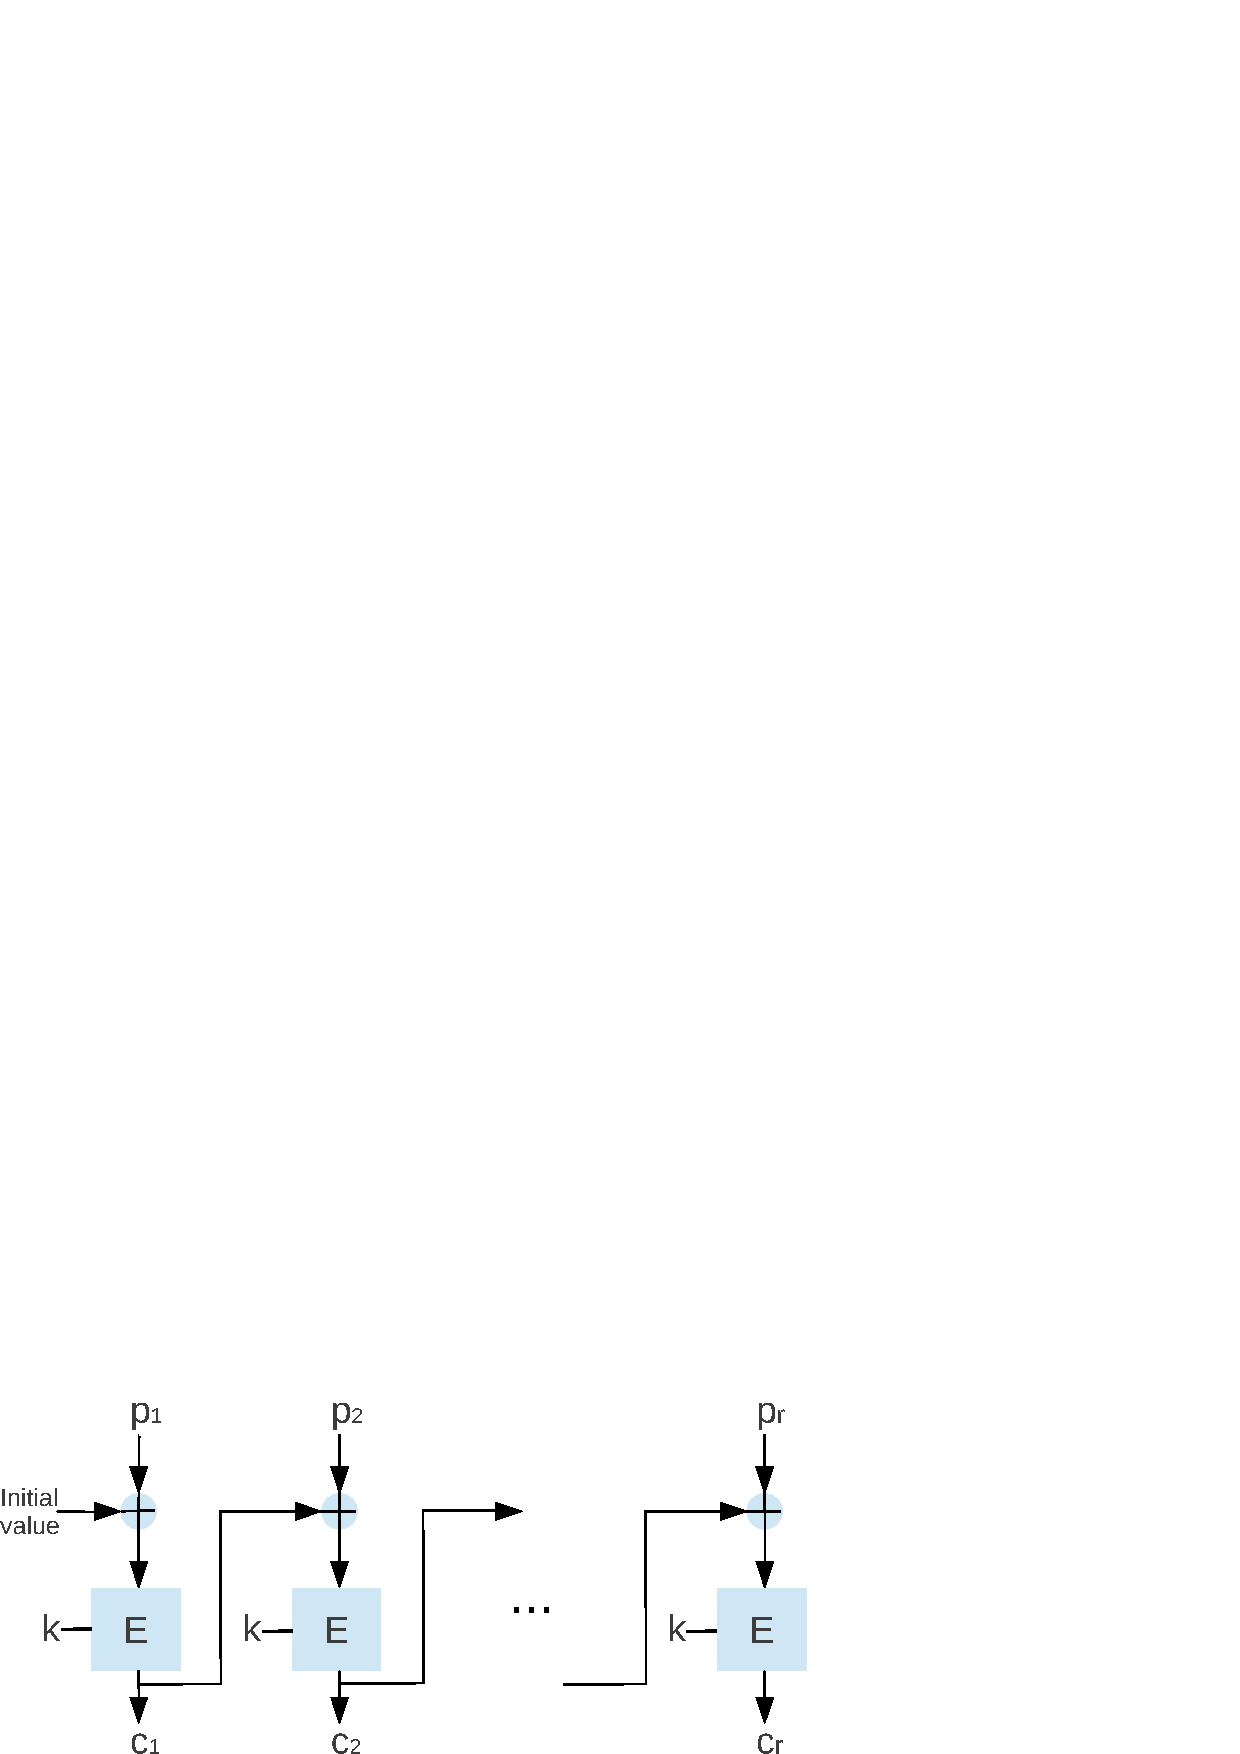
\includegraphics[scale=0.8]{Pictures/CBC_En.pdf}  
\caption{Workflow of the CBC encryption. Adapted from \cite{DBLP:reference/crypt/2011}.}\label{CBCEN}
\end{figure}
\subsubsection*{Decryption}
Mathematical description: $P_i=C_{i-1}\oplus D_K(C_i)$.\\
Figure \ref{CBCDE} shows the decryption workflow of CBC. It's the reverse of encryption. At the beginning the mode will be initialized with IV or in \texttt{Set\_IV()} reinitialized. A ciphertext block $C_1$ will be decrypted and the output will be XORed with $C_0$. The result of the XOR operation is the plaintext block $P_1$. The next ciphertext block $C_2$ will be decrypted and the output will be XORed with $C_1$ as $P_2$ and so on. 
\begin{figure}[h]
\centering
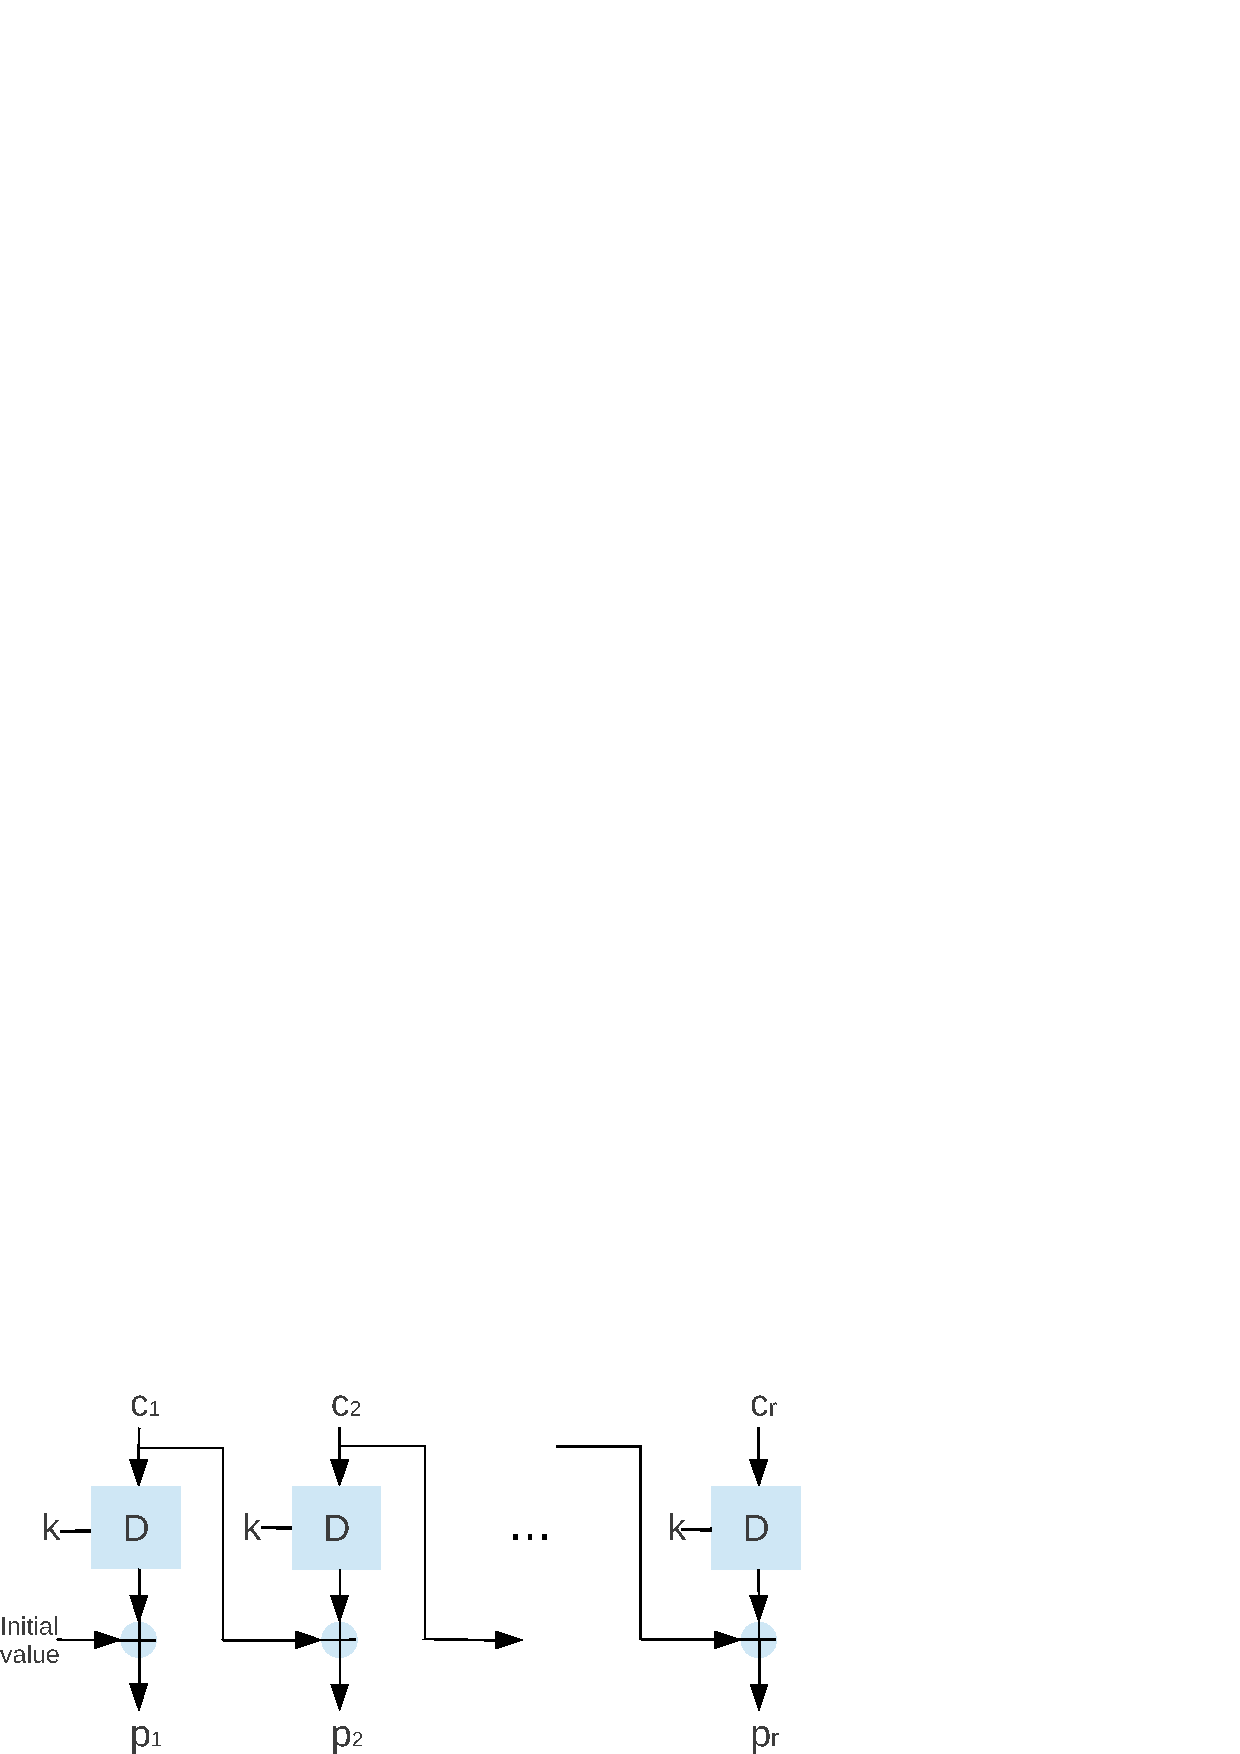
\includegraphics[scale=0.8]{Pictures/CBC_De.pdf} 
\caption{Workflow of the CBC decryption. Adapted from \cite{DBLP:reference/crypt/2011}.}\label{CBCDE}
\end{figure}
\subsubsection*{Purpose of Use}
\begin{itemize}
\item \textbf{Data Encryption}\\
Since there can be no error by synchronization in this mode, it is useful for data encryption. However it can lead to bit errors (through defective hardware or the like). One bit error in a ciphertext block $C_i$ can influence the plaintext block $P_i$ and also the related bit in next plaintext block $P_{i+1}$.
\item \textbf{Message Integrity Testing}\\
In order to test the integrity of a message, we encrypt the message and only need to remember two ciphertext blocks: $C_0=IV$ and $C_n$. The remaining ciphertext blocks are not required. Now we can certify at any time by encrypting the message $M$ to $C'_n$ with the start value $C_0$ and compare $C_n$ with $C'_n$, whether the message is changed or not. If $C_n=C'_n$, then the message $M$ is the original one, otherweise at least one of $IV$, $C_n$ or $M$ is changed. "Changed" is understood as accidental tipping of one or more bits.
\item \textbf{Message Authenticity Testing}\\
Supposed that you tell Alice a key, who you'd never met before. And one day you want to meet Alice to exchange secret data. To ensure that the people at the meeting point is really Alice, you bring a message $M$ and a randomly start value $IV$. You ask Alice to encrypt the message to $C'_n$ with the key and the start value. If $C'_n$ agrees with your computed $C_n$ (neither you nor Alice has told anyone the key), then the person is with significant propability to be Alice. If the two values are not the same, then the person is not Alice.
\item \textbf{Notice: The CBC-Mode is only secure when the exchanged messages are at the same length.} So users should pay attention to use the CBC Mode.
\end{itemize}
%%%%%%%%%%%%%%%%%%%%%%%%%%%%%%%%%%%%%%%%%%%%%%%%%%%%%%%%%
%%%%%%%%%%%%%%%%%%%%%%%%%%%%%%%%%%%%%%%%%%%%%%%%%%%%%%%%%
\section{BPS}
\subsubsection*{Package: Crypto.Symmetric.Mode.BPS}
BPS is a generic format-preserving symmetric encryption algorithm, which can cipher short or long string of characters from any given set, e.g. credit card numbers.
\subsubsection*{Encryption and Decryption}
The main process is similar to the CBC mode with an IV set to 0.
Internally a 8-round encryption is used. The plaintext will be divided into two sub-strings $L,R$ of similar length, i.e. $P=L||R$, and each of them will be updated in turn \cite{BPS}. Decryption is also composed of 8 rounds. They work as shown in Figure \ref{BPSED}.\\
\begin{figure}[htp]
\center
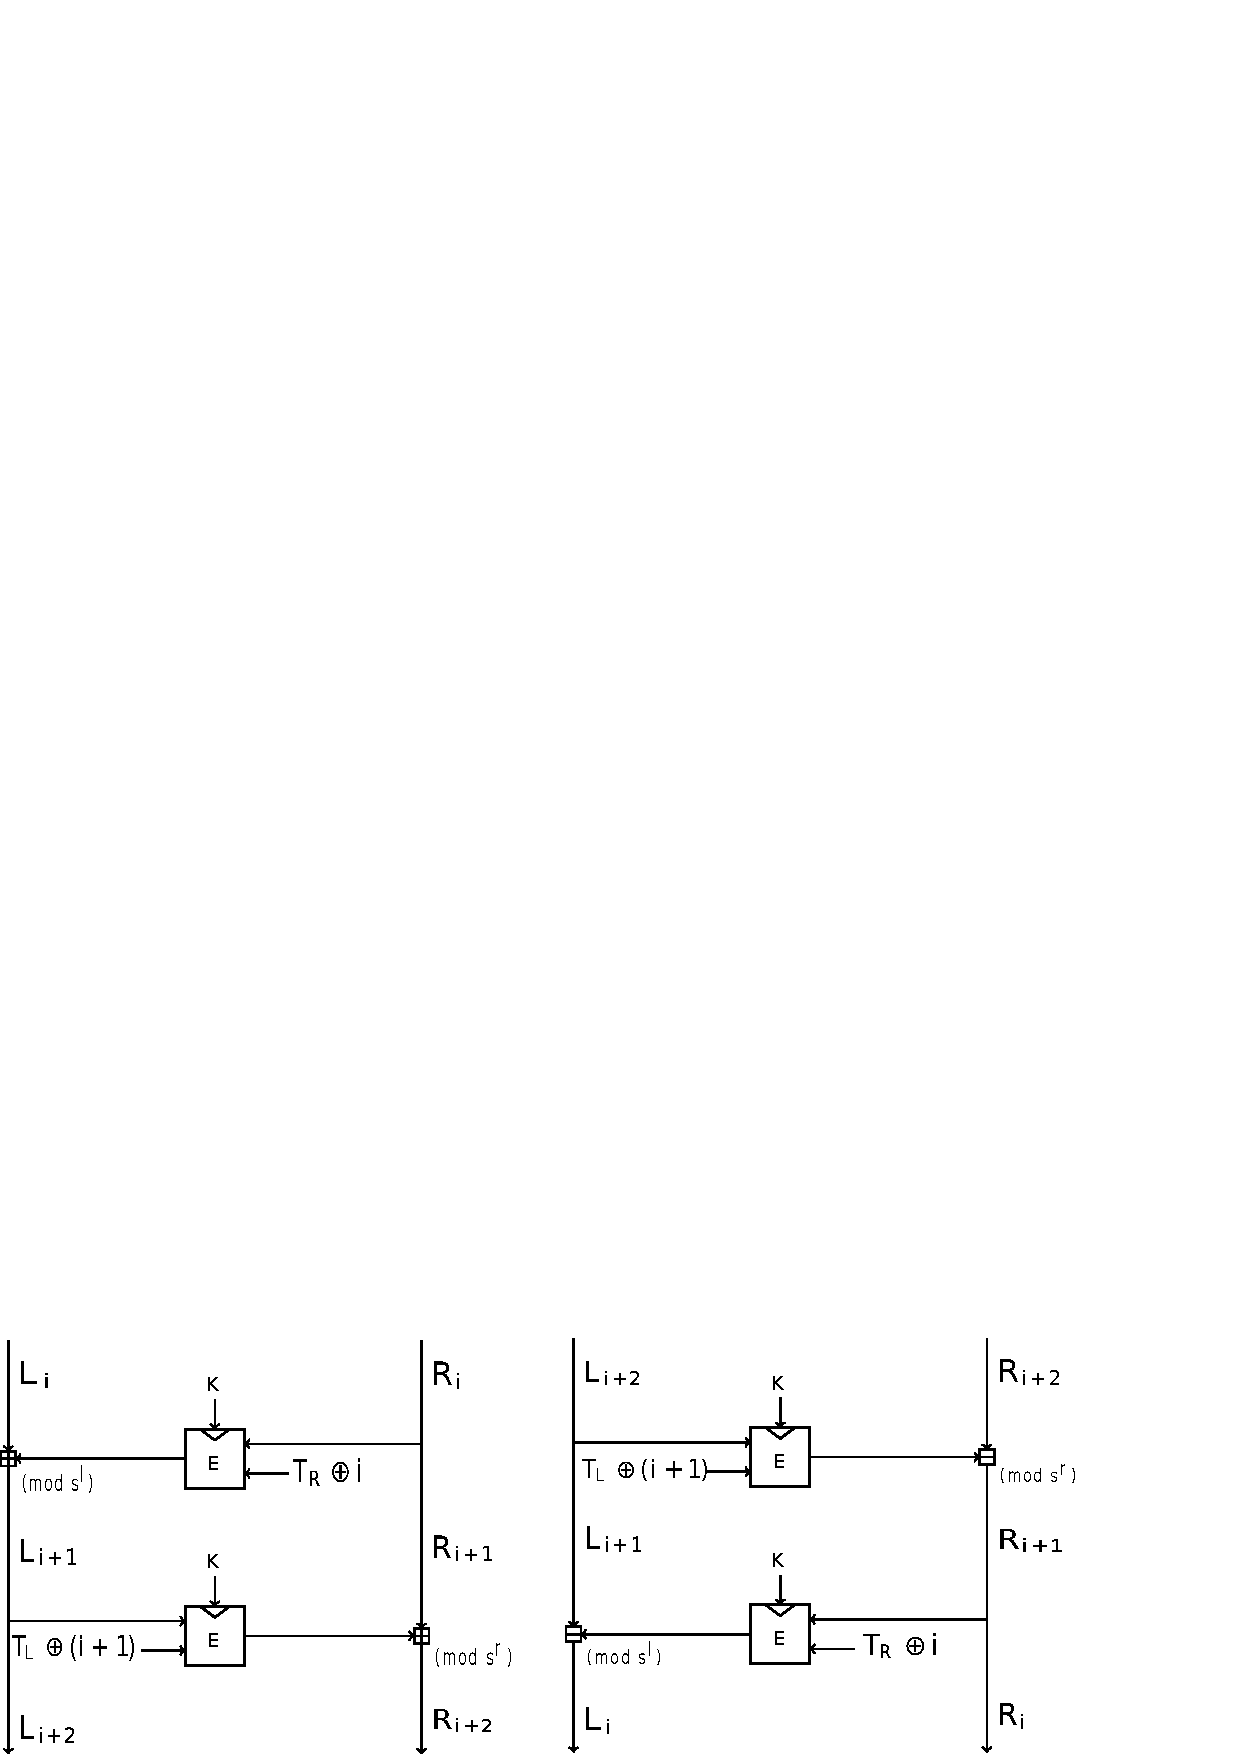
\includegraphics[scale=0.8]{Pictures/BPS_En_De.pdf} 
\caption{Workflow of the internal encryption (Left) and decryption (Right) in the BPS. \cite{BPS}}\label{BPSED}
\center
\end{figure}
\subsection*{Remarks}
\begin{itemize}
\item One advantage of BPS is its adaptability, all the block cipher and hash
function standardized primitives (TDES, AES or SHA-2) can be used as basic internal bricks \cite{BPS}. 
\item The internal tweak values is useful to avoid some kind of dictionary attacks \cite{BPS}. Indeed, if no tweak is used, a third party could build a dictionary of plaintext / ciphertext pairs and find with good probability the eavesdropped encrypted PANs (Personal Account Numbers), this attack works when the amount of data is small, which is particularly the case for an array of numbers encryption \cite{BPS}. "Using random tweak will render this dictionary technique useless as one dictionary per tweak value would be required" \cite{BPS}.
\item An essential quality of BPS is its efficiency. Due to that the input key for all the block cipher internal calls is constant, this requires only one internal cipher key per BPS encryption, which saves a lot of operations and time \cite{BPS}. Moreover, w = 8 rounds is recommanded, it makes the whole encryption process very efficient \cite{BPS}.
\end{itemize}
%%%%%%%%%%%%%%%%%%%%%%%%%%%%%%%%%%%%%%%%%%%%%%%%%%%%%%%%%
%%%%%%%%%%%%%%%%%%%%%%%%%%%%%%%%%%%%%%%%%%%%%%%%%%%%%%%%%
\section{Cipher Feedback Mode (CFB)}\label{CipherFeedbackMode}
\subsubsection*{Package: Crypto.Symmetric.Mode.CFB}
The cipher feedback (CFB) mode, a close relative of CBC, makes a block cipher into a self-synchronizing stream cipher \cite{DBLP:reference/crypt/2011}.
\begin{figure}[htp]
\center
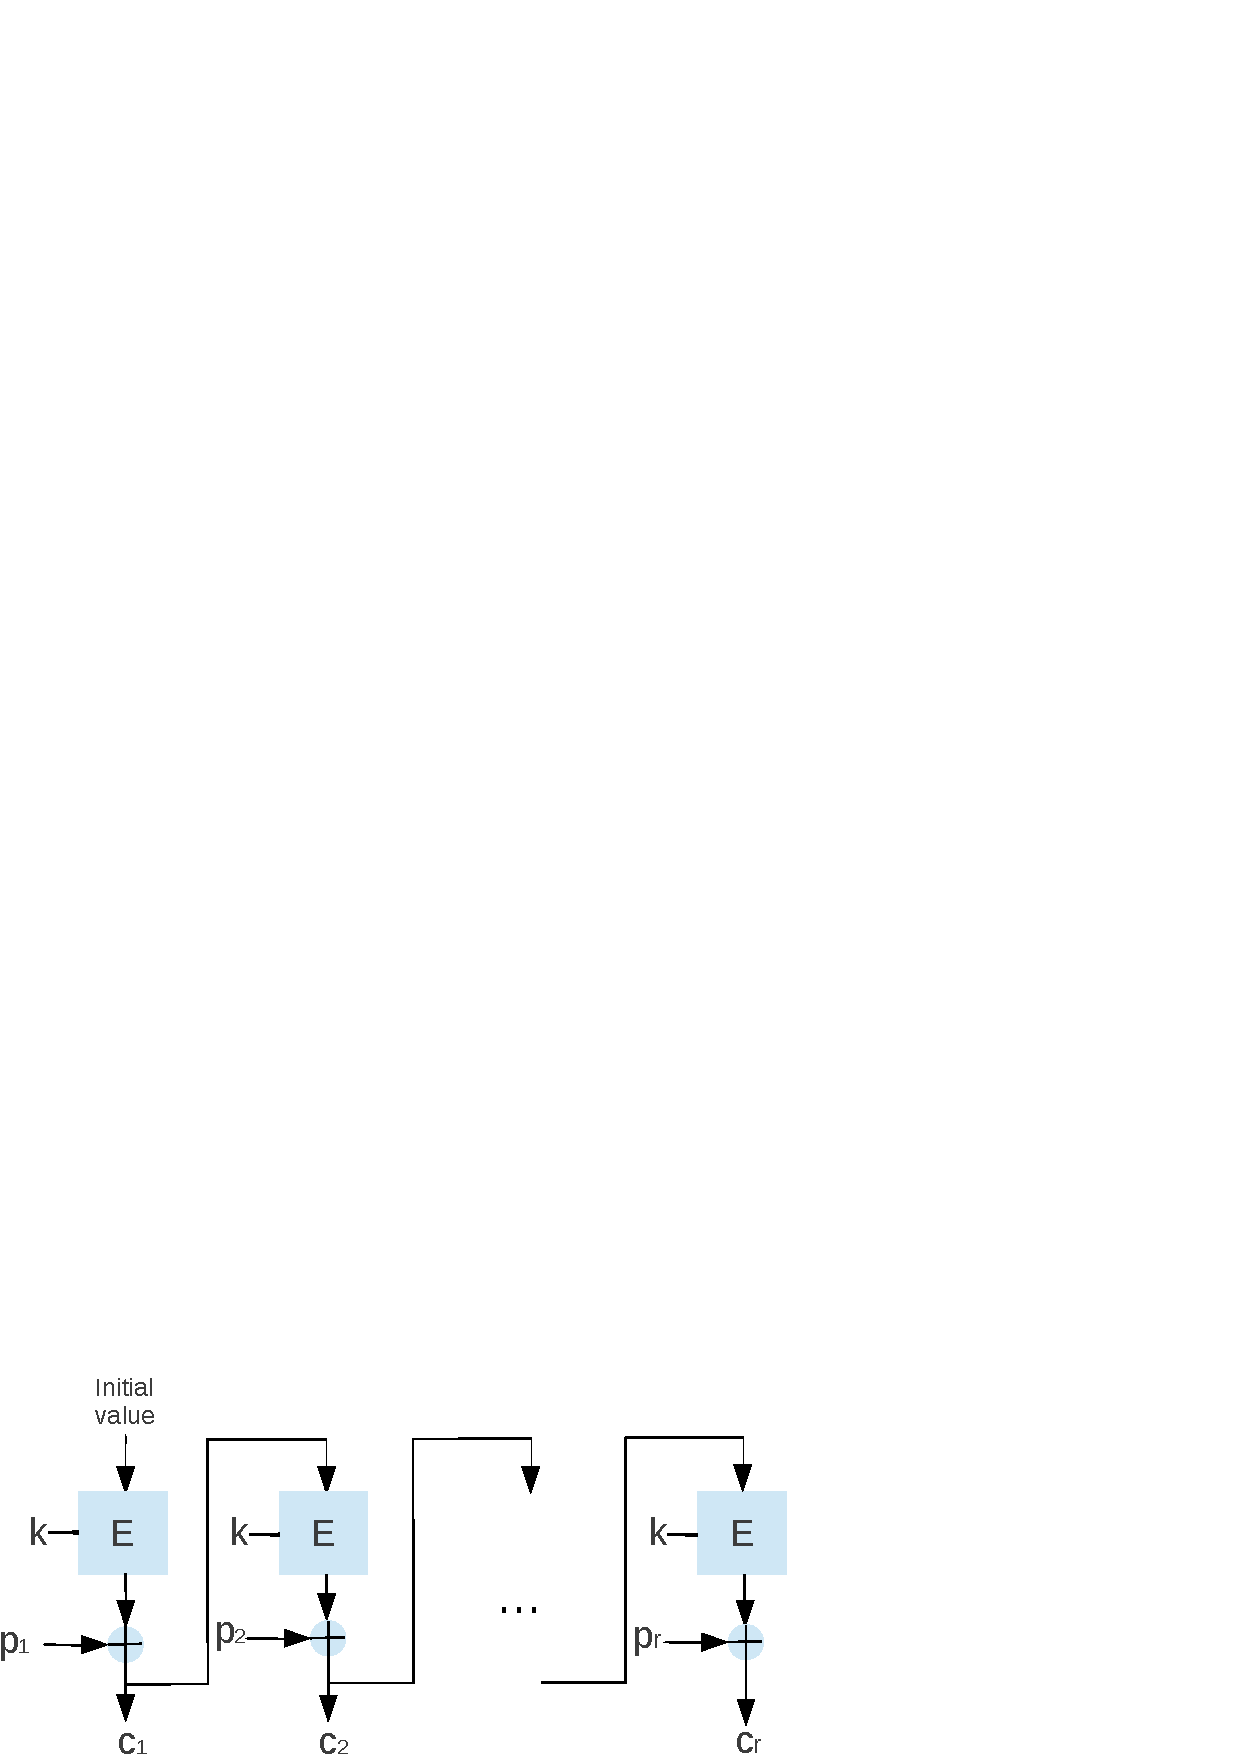
\includegraphics[scale=0.8]{Pictures/CFB_En.pdf} 
\caption{Workflow of the CFB encryption. Adapted from \cite{DBLP:reference/crypt/2011}.}\label{CFBEN}
\center
\end{figure}\\
\subsubsection*{Encryption}
Mathematical description : $C_i=E_K(C_{i-1})\oplus P_i$, $C_0=IV$.\\
Figure \ref{CFBEN} shows the workflow of encryption in CFB. By initialization the start value IV will be stored as $C_0$. To encrypt a $n$ bit ($n<$ Block'Size) message, it will be copied in the plaintext block, and then padded with zeros. To encrypt a plaintext block $P_1$, the start value $C_0$ will be encrypted at first, and then XORed with $P_1$ and stored as $C_1$. Following plaintext blocks will be processed iteratively until the complete message is encrypted.
\subsubsection*{Decryption}
Mathematical description : $P_i=E_K(C_{i-1})\oplus C_i$, $C_0=IV$.\\
As shown in Figure \ref{CFBDE}, the decryption in CFB makes use of the encryption algorithm. At the beginning the mode will be initialized or through \texttt{Set\_IV()} reinitialized. To decrypt a ciphertext block $C_i$, $C_{i-1}$ will be decrypted at first and then XORed with $C_i$. The output of the operation is $P_i$.
\begin{figure}[h]
\centering
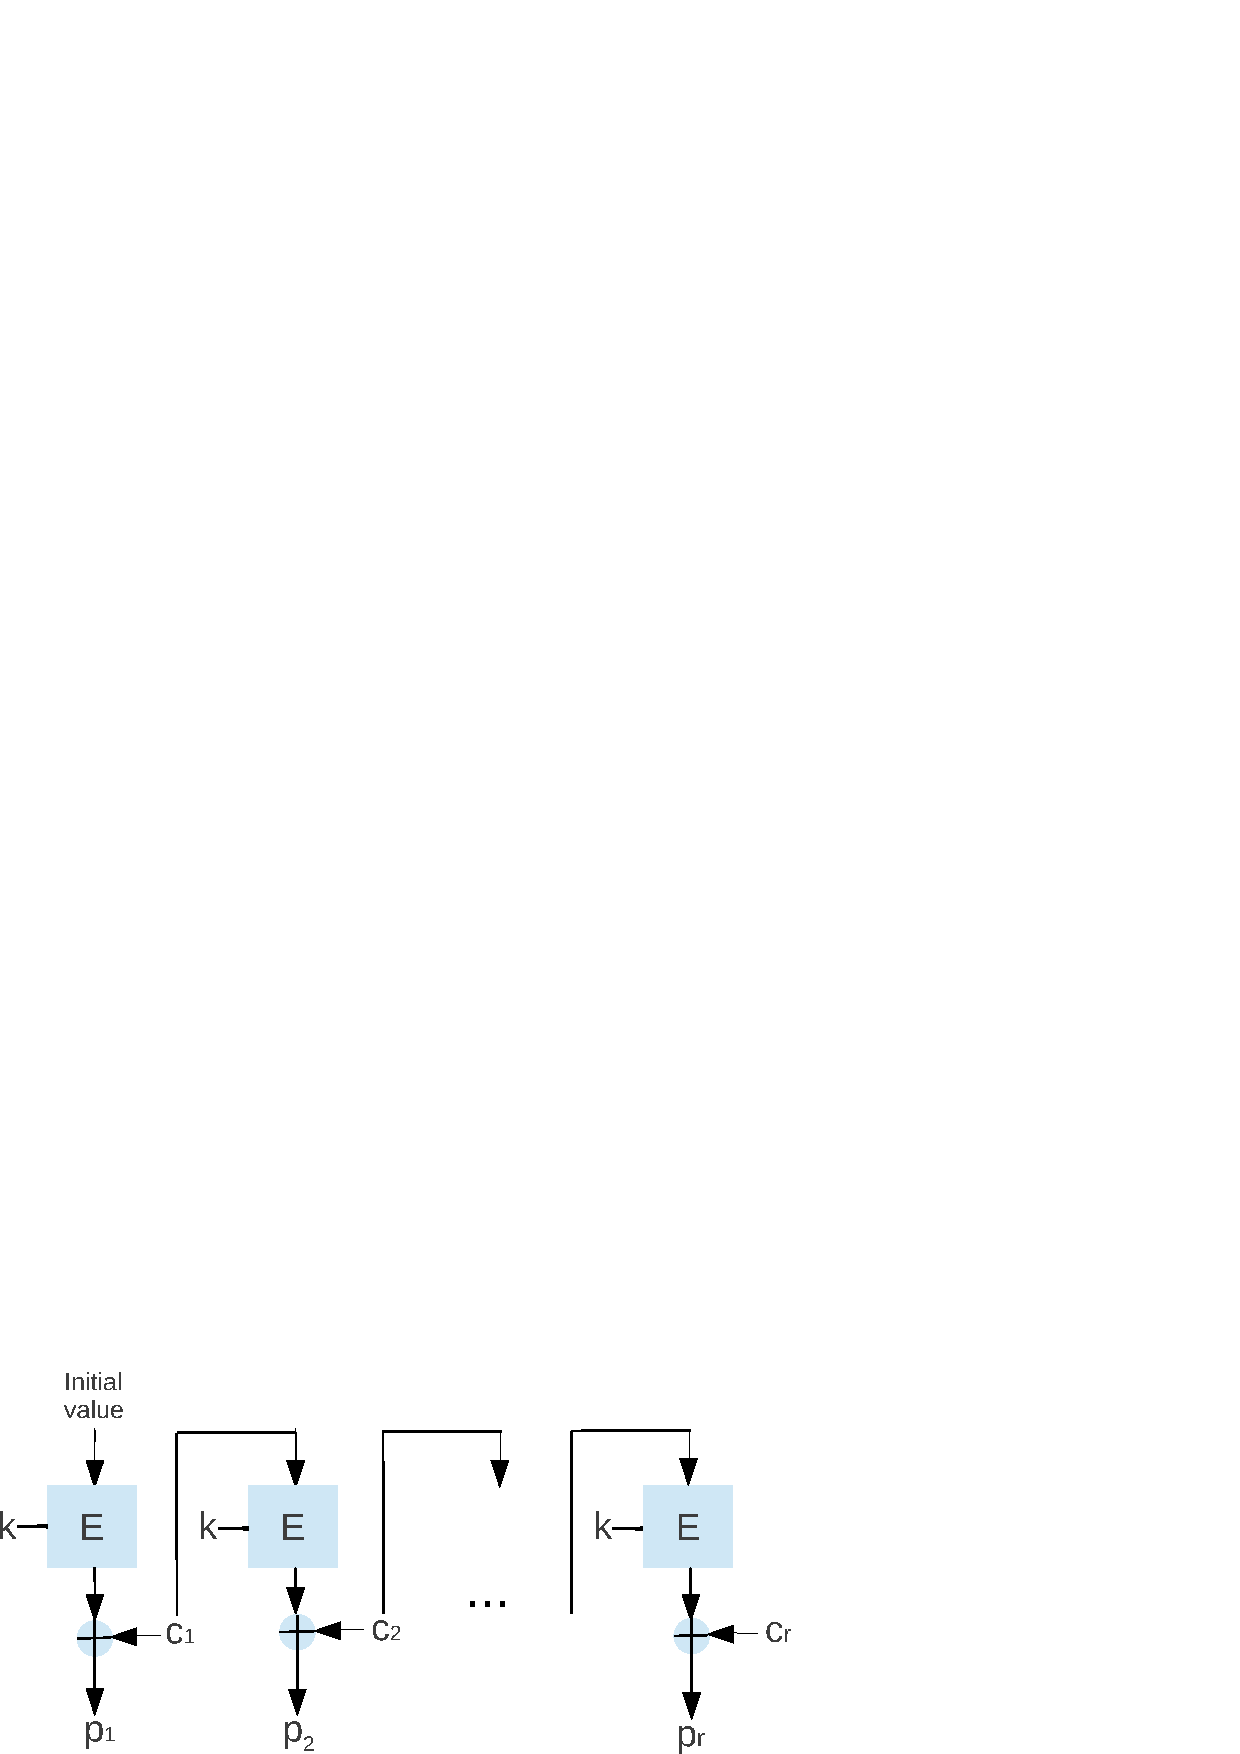
\includegraphics[scale=0.8]{Pictures/CFB_De.pdf} 
\caption{Workflow of the CFB decryption. Adapted from \cite{DBLP:reference/crypt/2011}.} \label{CFBDE}
\end{figure}
\subsubsection*{Remarks}
In comparison with CBC-Mode, which can be used when a complete data block exists, CFB-Mode can be used to encrypt not only data but also bytes (8-CFB). Therefore it is mainly used for encryption of byte streams (e.g. Remote shell).\\
In n-CFB-Mode:
\begin{itemize}
\item an error in plaintext will affect the following complete ciphertext and in decryption it goes backward.
\item an error in ciphertext $C_i$ will affect the plaintext block $P_i$ and also the following $\frac{m}{n}-1$ plaintext blocks, where $m$ is the size of the message.
\item An aggressor can change the message bits in the last ciphertext block without being found.
\end{itemize}
%%%%%%%%%%%%%%%%%%%%%%%%%%%%%%%%%%%%%%%%%%%%%%%%%%%%%%%%%
%%%%%%%%%%%%%%%%%%%%%%%%%%%%%%%%%%%%%%%%%%%%%%%%%%%%%%%%%
\section{Counter Mode (CTR)}\label{CounterMode}
\subsubsection*{Package: Crypto.Symmetric.Mode.CTR}
In Counter Mode the feedback isn't dependent on plaintext, but on a counter, which will be increased by 1 after every encryption. Note that the nonce in Figure \ref{CTREN} and Figure \ref{CTRDE} is the same thing as the initial vector (IV) in other graphs. 
\subsubsection*{Encryption}
Mathematical description : $C_i=P_i\oplus E_K(IV+i-1)$.\\
In Figure \ref{CTREN} the counter is initialized at first. The current counter $IV+i-1$ of each block is encrypted, the output is then XORed with plaintext block $P_i$, and the result is $C_i$.
\begin{figure}[h]
\centering
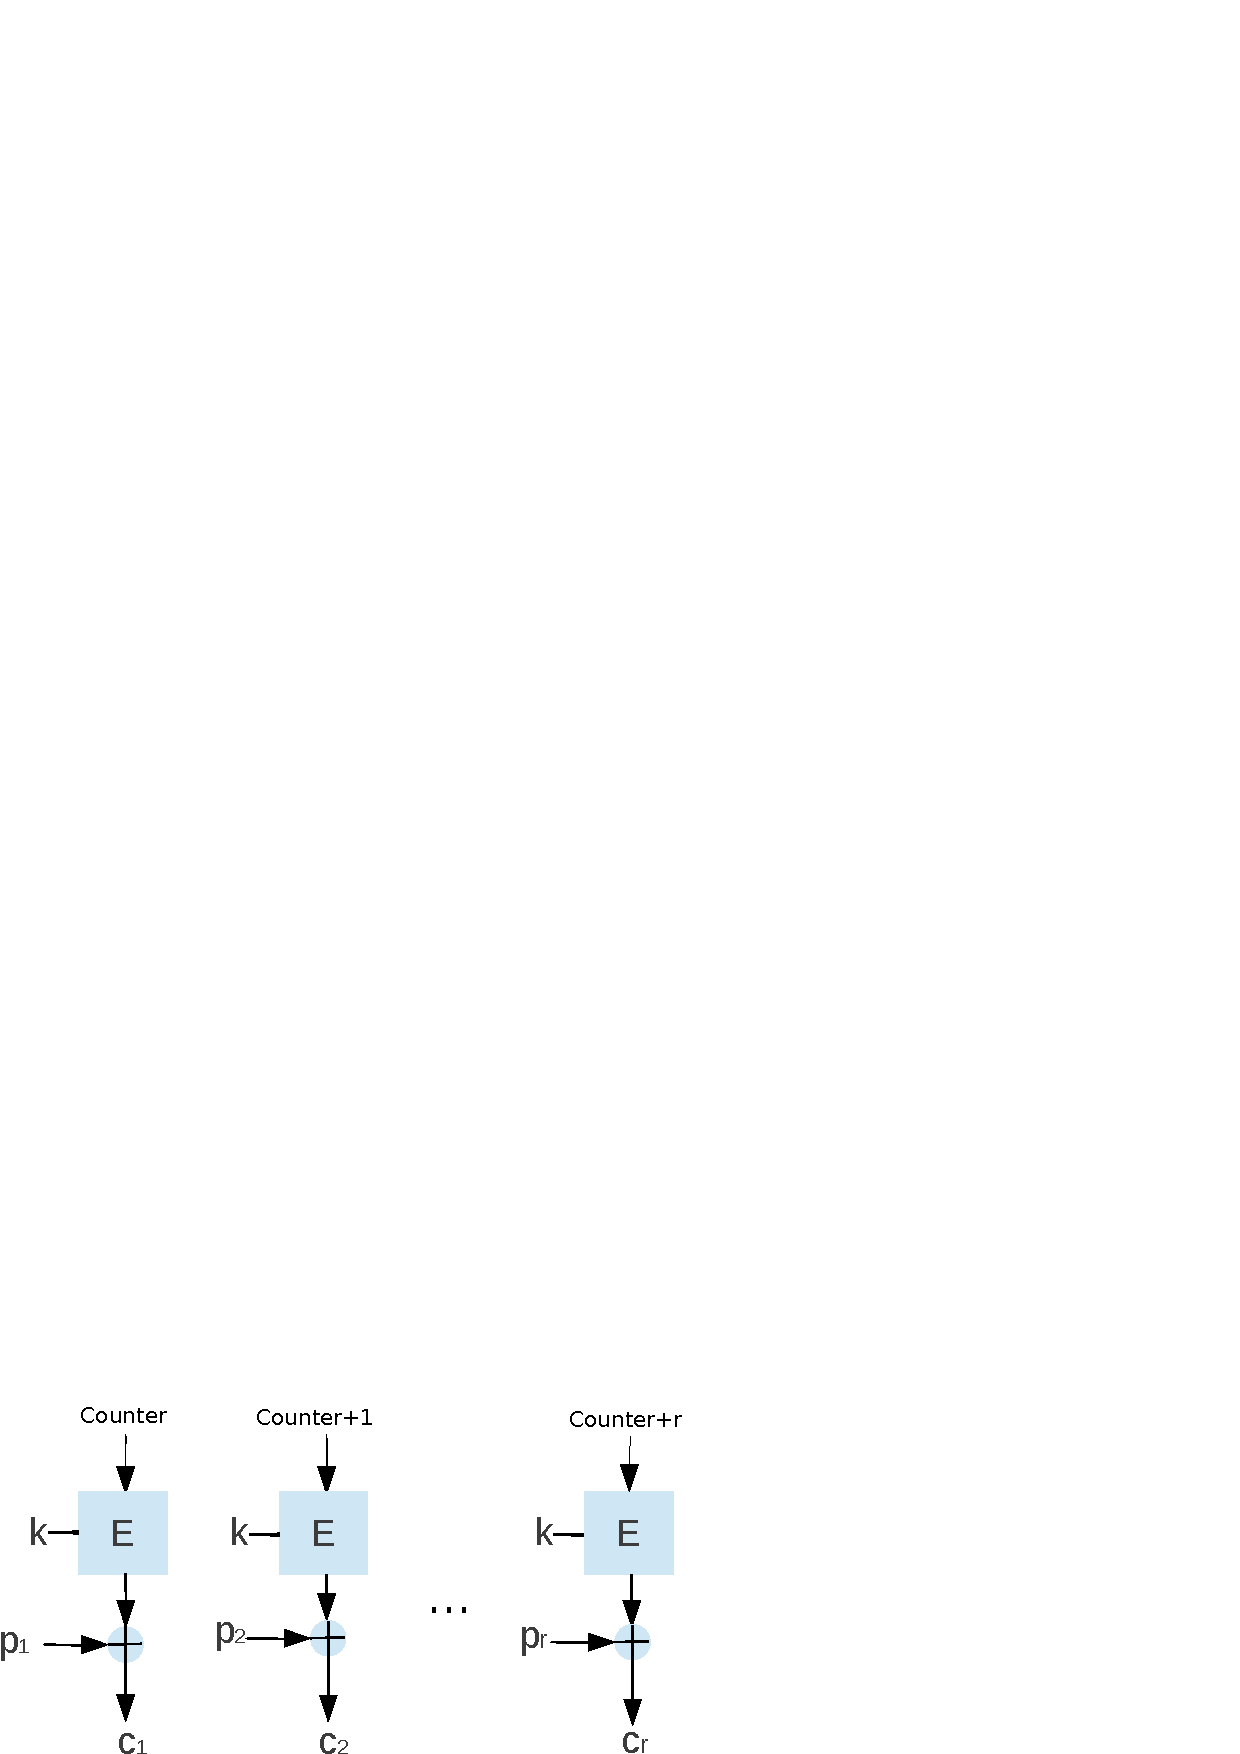
\includegraphics[scale=0.8]{Pictures/CTR_En.pdf} 
\caption{Workflow of the CTR encryption. Adapted from \cite{DBLP:reference/crypt/2011}.}\label{CTREN}
\end{figure}
\subsubsection*{Decryption}
Mathematical description : $P_i=C_i\oplus E_K(IV+i-1)$.\\
Note that in Figure \ref{CTRDE} the encryption algorithm is used in decryption.
After initialization counter $IV+i-1$ will be encrypted, then the output will be XORed with $C_i$ and the result is $P_i$. It is done iteratively until the last block.
\begin{figure}[h]
\centering
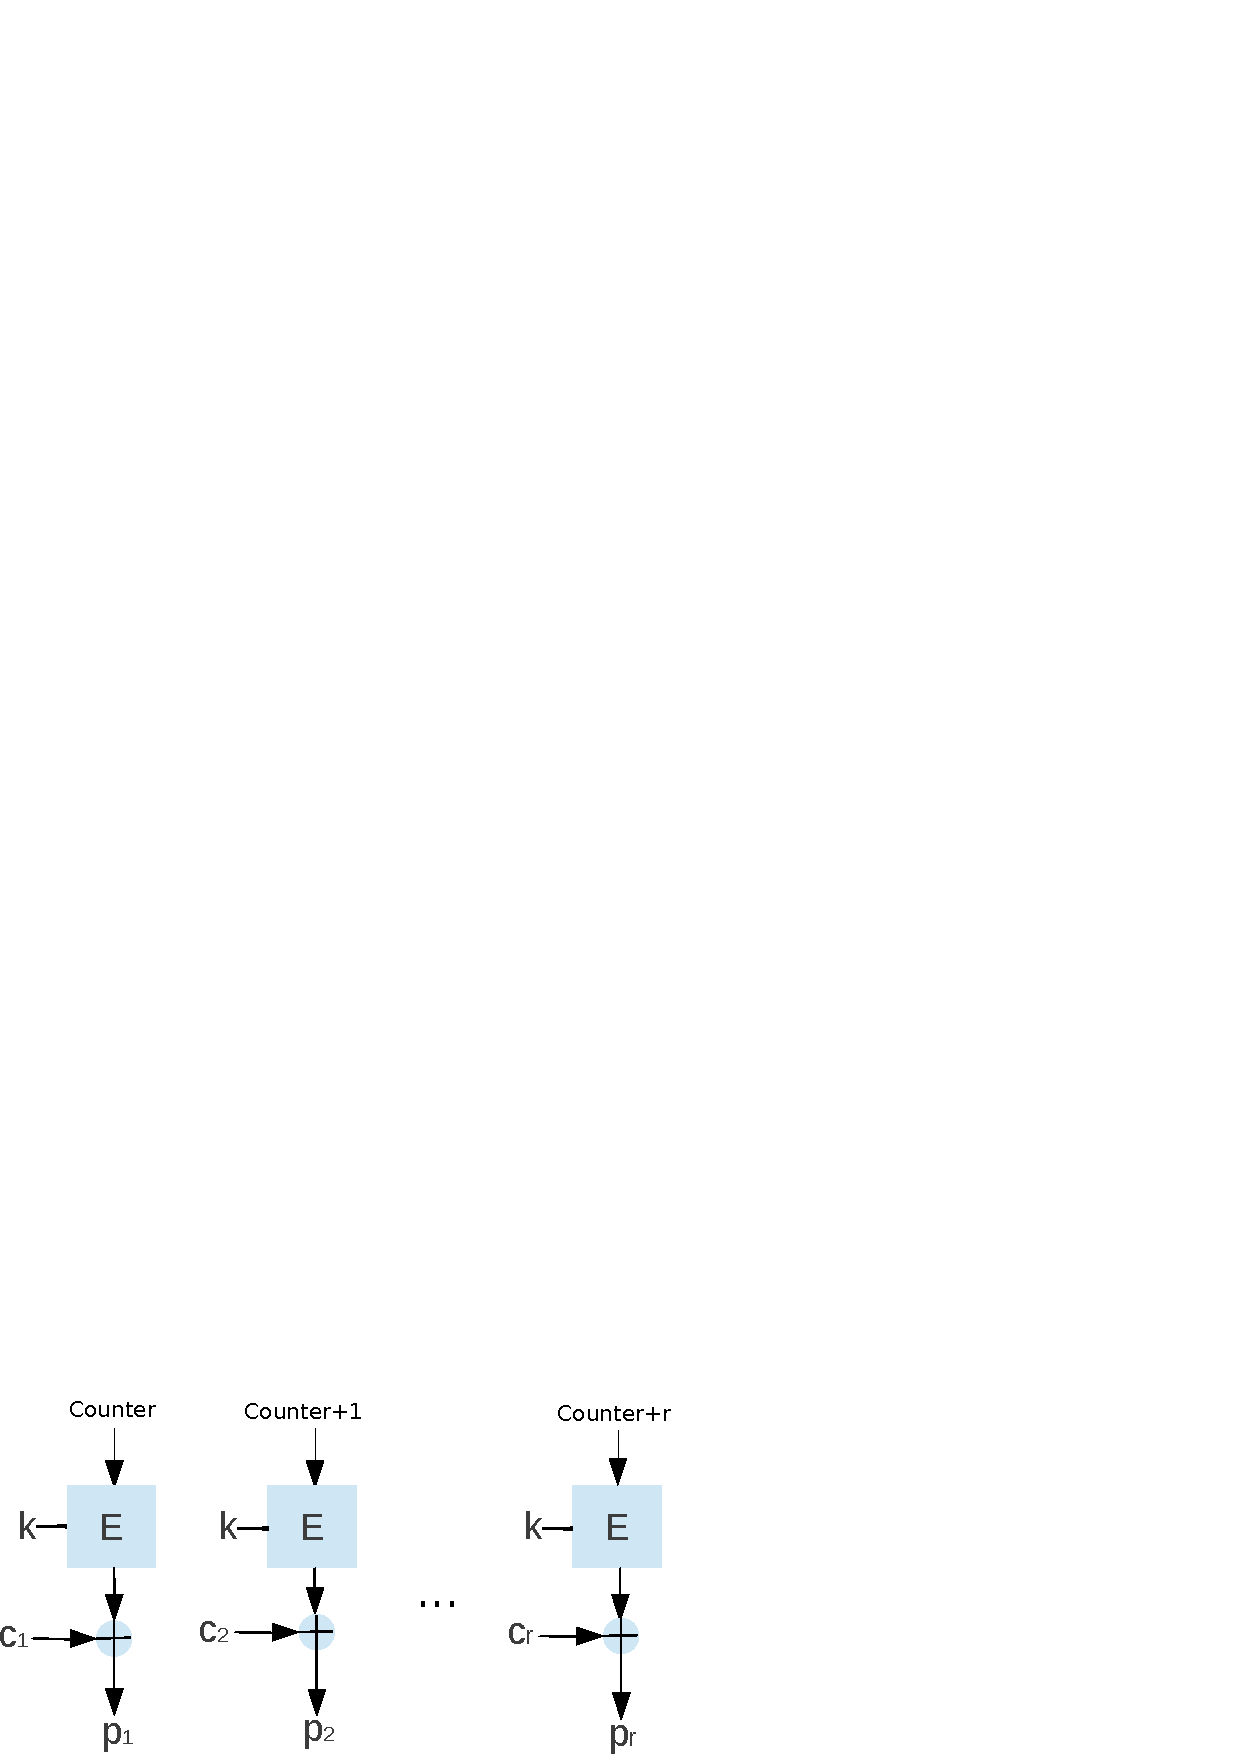
\includegraphics[scale=0.8]{Pictures/CTR_De.pdf} 
\caption{Workflow of the CTR decryption. Adapted from \cite{DBLP:reference/crypt/2011}.}\label{CTRDE}
\end{figure}
\subsubsection*{Remarks}
\begin{itemize}
\item \textbf{En-/Decryption of Messages with Random Access}\\
Since that the counter mode is used to decrypt individual ciphertext block, this procedure is suitable for decryption of data with random access e.g. Database.
\item \textbf{Parallel En-/Decryption}\\
Parallelization is possible when man calculates an interval from the start value (IV) and the length of the message is $L$: $[IV\cdots IV+L]$. The interval is decomposed in max. $L$ disjunktive part intervals. Then the message blocks in the part intervals can be en-/decrypted parallel.
\item \textbf{Phasic "High Speed" Encryption}\\
This is a professional function that based on "Low-Level-API" (\ref{Low-Level}) of CTR mode. Please use this only when you konw what it does. In CTR mode it is possible to generate random keystream bits without a message block to be needed. When you generate enough keystream bits with the CTR mode, then you are able to encrypt the messages very quickly through being XORed with the already produced keystream bits.
\end{itemize}
\subsubsection*{Notice:}
\begin{itemize}
\item A bit error in plaintext will influence only one bit in ciphertext and vice versa.
\item Manipulation on plaintext is clear, because every change in ciphertext influences directly the plaintext.
\item Error in Synchronization (Alice and Bob are in different counter states) can not be solved. 
\end{itemize}
\subsubsection*{Low-Level-API}\label{Low-Level}
This API can be used only when you know exactly what it does.
\begin{lstlisting}{}
  procedure Next_Block(Keystream : out Block);
\end{lstlisting}
Mathematical description : $C=E_K(Counter)$; $Counter:=Counter+1$.\\
It encrypts the internal counter to $C$, and the counter will be increased by 1.
%%%%%%%%%%%%%%%%%%%%%%%%%%%%%%%%%%%%%%%%%%%%%%%%%%%%%%%%%%%%%
%%%%%%%%%%%%%%%%%%%%%%%%%%%%%%%%%%%%%%%%%%%%%%%%%%%%%%%%%%%%%
\section{Output Feedback Mode (OFB)}\label{OutputFeedbackMode}
\subsubsection*{Package: Crypto.Symmetric.Mode.OFB}
The OFB mode converts a blockcipher in a stream cipher like the CTR mode. That is, the internal feedback is independent from the plaintext.
\subsubsection*{Encryption}
Mathematical description : $C_i=P_i\oplus K_i\,,\, K_i=E_K(K_{i-1})$.\\
In Figure \ref{OFBEN} shows the workflow of encryption in OFB.
$IV$ is assigned to an internal keystream block $K_0$. Block $K_{i-1}$ will be encrypted to $K_i$ and then XORed with $P_i$, and the result of the operation is ciphertext block $C_i$.
\begin{figure}[h]
\centering
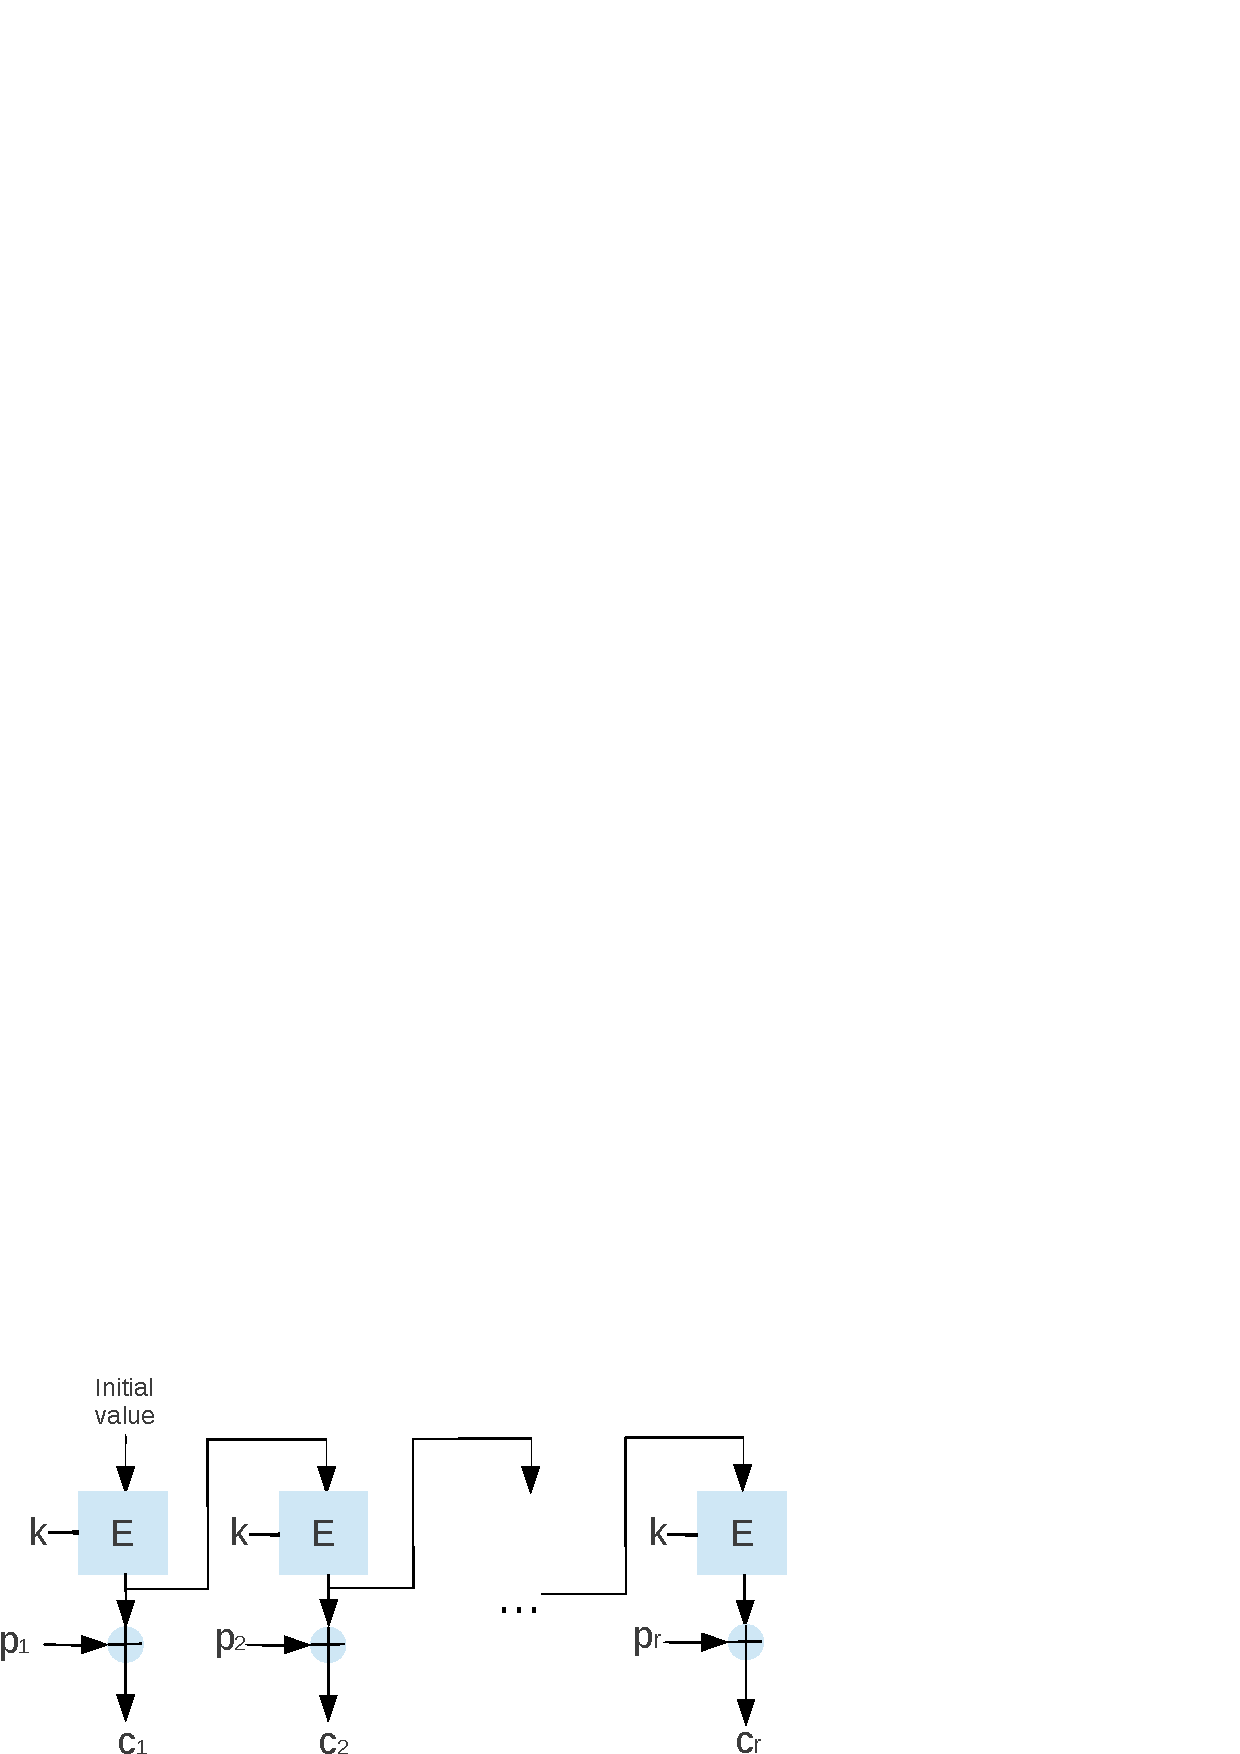
\includegraphics[scale=0.8]{Pictures/OFB_En.pdf} 
\caption{Workflow of the OFB encryption. Adapted from \cite{DBLP:reference/crypt/2011}.}\label{OFBEN}
\end{figure}
\subsubsection*{Decryption}
Mathematical description : $P_i=C_i\oplus K_i\,,\, K_i=E_K(K_{i-1})$.\\
The algorithm encryption is used in decryption as shown in Figure \ref{OFBDE}. The keystream block $K_0$ is initialized with the start value $IV$ or reinitialized by \texttt{Set\_IV()}. $K_{i-1}$ will be encrypted to $K_i$ and XORed with $C_i$. The result of the operation is the plaintext block $P_i$. These ciphertext blocks are decrypted in the same sequence in which they are generated.
\begin{figure}[h]
\centering
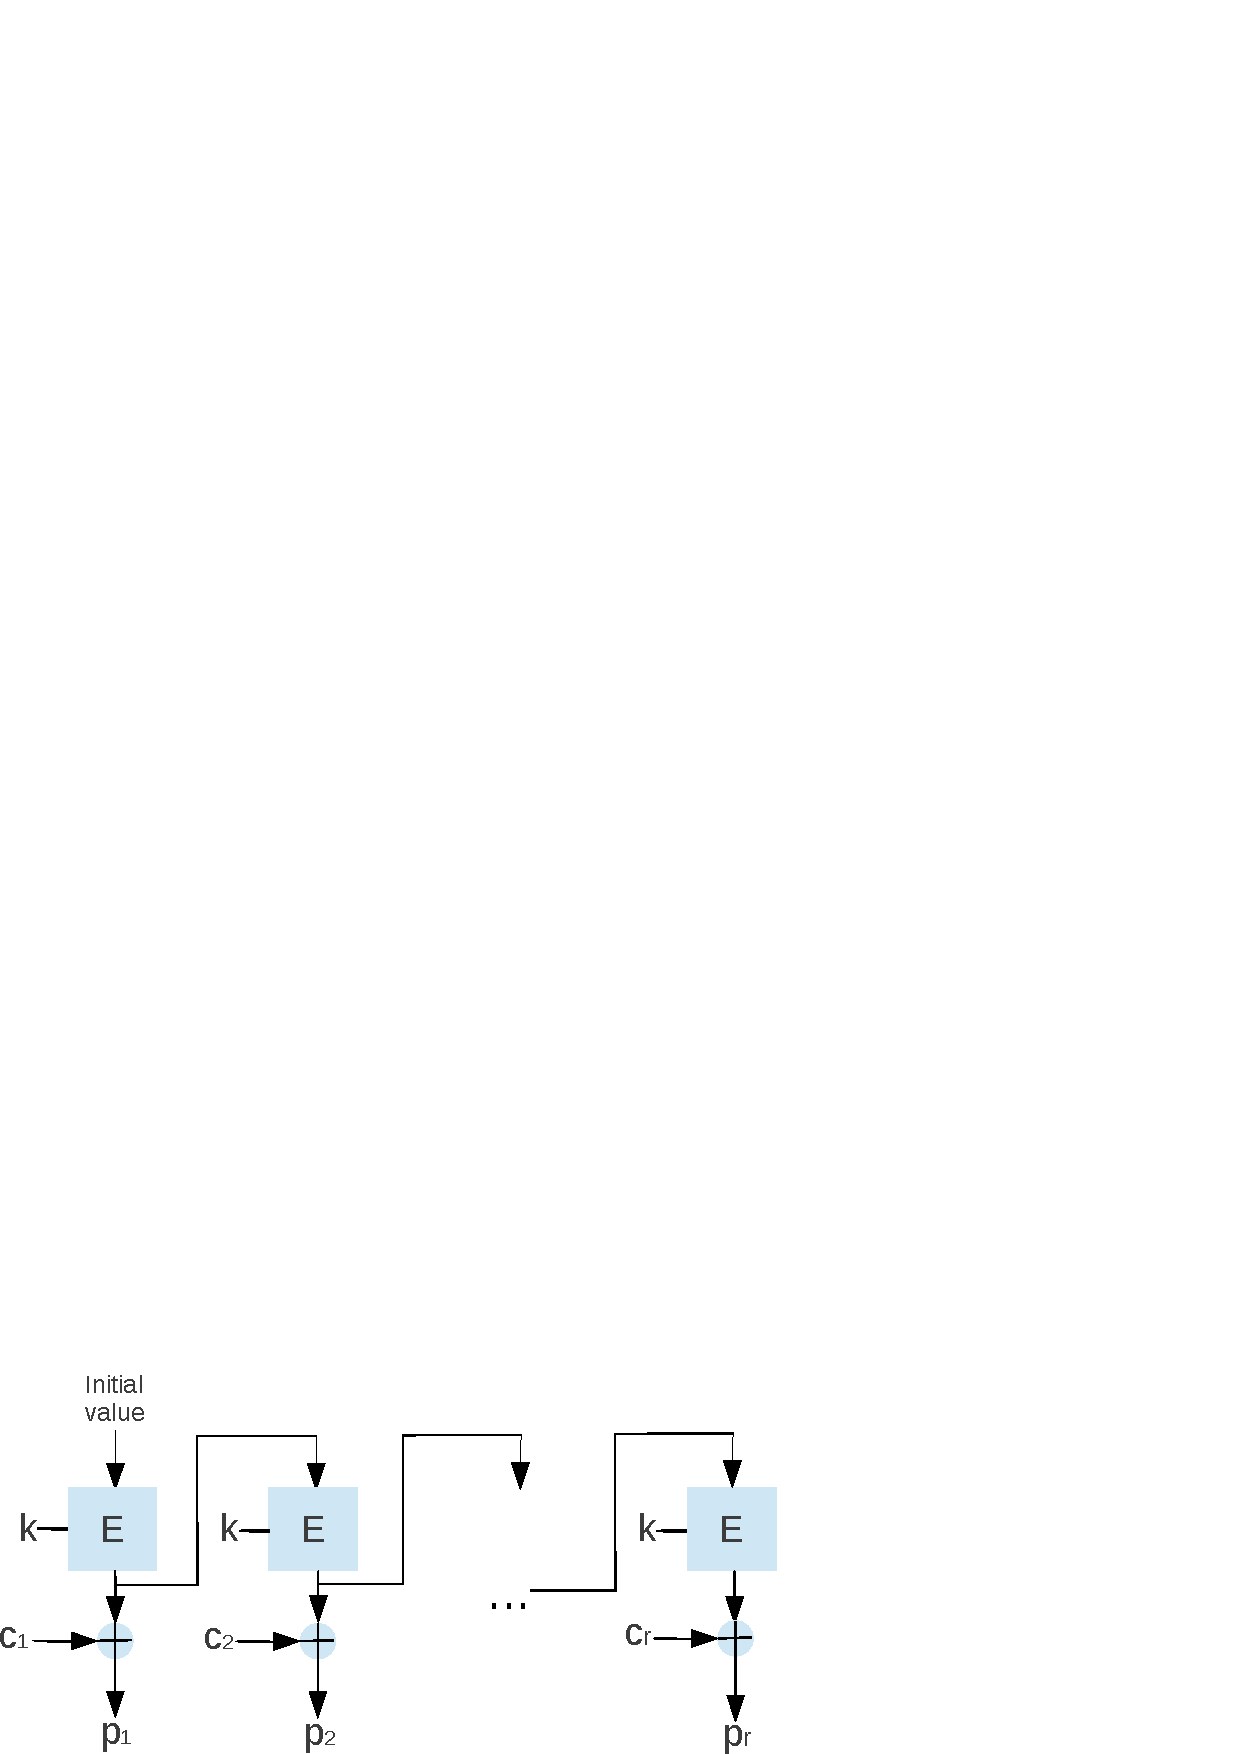
\includegraphics[scale=0.8]{Pictures/OFB_De.pdf} 
\caption{Workflow of the OFB decryption. Adapted from \cite{DBLP:reference/crypt/2011}.}\label{OFBDE}
\end{figure}
\subsubsection*{Remarks}
With the "Low-Level-API" (\ref{Low-Level-OFB}) users can generate a keystream without plaintext blocks. Thereby they can encrypt the plaintext blocks very fast. For example it will be possible to generate keystream blocks at night and then encrypt plaintext blocks in the day time. So this mode is very suitable when phasic plaintext blocks should be encrypted quickly.
\subsubsection*{Notice:}
\begin{itemize}
\item The keystream repeats at any time. That is, $\exists L:K_0=K_L$. Supposed $m$ is the block size in bits, then the average length of a cycle goes to $2^m-1$ bits.
\item A bit error in plaintext will influence one bit in ciphertext and vice versa.
\item Manipulation on plaintext is clear, every change in ciphertext influences directly the plaintext.
\item Error in synchronization (Alice and Bob are in different counter states) can not be solved. 
\end{itemize}
\subsubsection*{Low-Level-API}\label{Low-Level-OFB}
The following API can be used only when you know what it does.
\begin{lstlisting}{}
  procedure Next_Block(Keystream : out Block);
\end{lstlisting}
Mathematical description : $K_i=E_K(K_{i-1})$.\\
During initialization the start value IV is stored as keystream block $K_0$. Every time when the \texttt{Next\_Block()} procedure is called, the keystream block $K_i$ will be encrypted to $K_{i+1}$ and resulted as keystream.
%%%%%%%%%%%%%%%%%%%%%%%%%%%%%%%%%%%%%%%%%%%%%%%%%%%%%%%%%%%
%%%%%%%%%%%%%%%%%%%%%%%%%%%%%%%%%%%%%%%%%%%%%%%%%%%%%%%%%%%
\section{Example}
\subsubsection*{CBC Mode}
\begin{lstlisting}{}
  with Crypto.Types;
  with Ada.Text_IO;
  with Crypto.Symmetric.Blockcipher_Tripledes;
  with Crypto.Symmetric.Mode.CBC;
  procedure Example_CBC_Mode is
	 use Ada.Text_IO; use Crypto.Types;
    package TDES renames Crypto.Symmetric.Blockcipher_Tripledes;
    -- use TDES in secure CBC mode
    package TDES_CBC is new Crypto.Symmetric.Mode.CBC(TDES);
	 use TDES_CBC;
    Key: B_Block192 := (16#00#, 16#00#, 16#00#, 16#00#, 16#00#, 
                        16#00#, 16#00#, 16#00#, 16#00#, 16#00#, 
                        16#00#, 16#00#, 16#00#, 16#00#, 16#00#, 
                        16#00#, 16#01#, 16#23#, 16#45#, 16#67#, 
                        16#89#, 16#ab#, 16#cd#, 16#ef#);
    IV: B_Block64 := (16#12#, 16#34#, 16#56#, 16#78#,
            	          16#90#, 16#ab#, 16#cd#, 16#ef#);
    --Plaintext
    P_String: String :="Now is the time for all.";
    --Plaintext will be divided in 3*64 bit blocks.
    P: array(1..3) of B_Block64 := 
			(To_B_Block64(To_Bytes(P_String(1..8))),
          To_B_Block64(To_Bytes(P_String(9..16))),
			 To_B_Block64(To_Bytes(P_String(17..24))));
    --Ciphertext
    C: array(0..3) of B_Block64;
    begin
      Init(Key, IV);    --1. Initialization
      C(0):= IV;        --1. Ciphertext block = start value
      for I in P'Range loop
	     Encrypt(P(I),C(I));  --Encryption
      end loop;
      --For decryption the start value will be 
      --reinitialized with the same value.
      Set_IV(C(0));         
      for I in P'Range loop
         Decrypt(C(I),P(I));   --Decryption
         Put(To_String(To_Bytes(P(I))));
      end loop;
  end Example_CBC_Mode;
\end{lstlisting}\\ \ \\
\subsubsection*{BPS Mode}
\begin{lstlisting}{}
  with Crypto.Symmetric.Mode.BPS;
  with Crypto.Symmetric.Blockcipher_AES128;
  with Crypto.Types; use Crypto.Types;
  with Ada.Text_IO; use Ada.Text_IO;
  procedure Example_BPS_Mode is
    package AES128 renames Crypto.Symmetric.Blockcipher_AES128;
    package BPS is new Crypto.Symmetric.Mode.BPS(AES128);
    use BPS;
    Key : B_Block128 := (16#12#, 16#34#, 16#56#, 16#78#,
	  	                 16#90#, 16#ab#, 16#cd#, 16#ef#,
		                 16#12#, 16#34#, 16#56#, 16#78#,
		                 16#90#, 16#ab#, 16#cd#, 16#ef#);
    IV : B_Block64 :=(16#12#, 16#34#, 16#56#, 16#78#,
		                16#90#, 16#ab#, 16#cd#, 16#ef#);
    Plaintext : BPS.Numerals(1..10) := (0,1,2,3,4,5,6,7,8,9);
    Ciphertext, P : BPS.Numerals(1..10);
    Result : Boolean := False;
  begin
    Init(Key, IV);
    Encrypt(Plaintext, Ciphertext);
    Decrypt(Ciphertext, P);
    for I in Plaintext'Range loop
       if Plaintext(I) = P(I) then
          Result := True;
       end if;
    end loop;
    if Result then
       Put_Line("OK");
    else
       Put_Line("Error"); 
    end if;
  end Example_BPS_Mode;
\end{lstlisting}
%  \chapter{Crypto.Symmetric.Mode.Oneway}
This generic package works with one-way blockciphers in one-way modes. It integrates a one-way block cipher with a feedback and also some easy operations ($+,xor$). A one-way mode will be initialized with a random start value (Initial Value (IV)). The ciphertext is therefore not only dependent on the used mode, plaintext and key, but also on the random start value. When users encrypt a plaintext twice with the same key in the same mode but different IVs, then they will get different ciphertexts, i.e. a oneway mode encrypts two plaintext blocks $P_1$ and $P_2$ with $P_1=P_2$ to two ciphertext blocks $C_1$ and $C_2$ with overwhelming probability that $C_1\neq C_2$. So that it is now possible to encrypt more messages with the same key.\\
\textbf{Notice: To decrypt a ciphertext the key and start value by encryption are required.} For this reason the start value should be always kept together with the related ciphertext. \textbf{The security of a mode is independent from the familarity of the start value.} Hense, man multiplies usually the start value with the ciphertext as the final output by attaching the ciphertext to the start value ($C'=IV||C$).
%%%%%%%%%%%%%%%%%%%%%%%%%%%%%%%%%%%%%%%%%%%%%%%%%%%%%%%%%%%%%%
%%%%%%%%%%%%%%%%%%%%%%%%%%%%%%%%%%%%%%%%%%%%%%%%%%%%%%%%%%%%%%
\subsubsection*{Remarks}
\begin{itemize}
\item In a oneway mode it goes similarly as in a normal mode. If a normal mode can be used also as a oneway mode, then you should still prefer oneway mode, because it's nimbler.  
\item The API of this package is the same as in normal modes (\ref{API-Mode}).
\item Supported oneway modes:
\begin{itemize}
\item Cipher Feedback Mode (CFB) (\ref{CipherFeedbackMode})
\item Counter Mode (CTR) (\ref{CounterMode})
\item Output Feedback Mode (OFB) (\ref{OutputFeedbackMode})
\end{itemize}
\end{itemize}
\subsubsection*{Example}
\begin{lstlisting}{}
  with Crypto.Types;
  with Ada.Text_IO;
  with Crypto.Symmetric.Oneway_Blockcipher_Twofish128;
  with Crypto.Symmetric.Mode.Oneway_CTR;
  procedure Example_Mode_Oneway is
	 use Ada.Text_IO; use Crypto.Types;
    package TF128 renames 
                  Crypto.Symmetric.Oneway_Blockcipher_Twofish128;
    package Twofish128 is new
                  Crypto.Symmetric.Mode.Oneway_CTR(TF128);
 	 use Twofish128;
    Key: B_Block128 := (16#2b#, 16#7e#, 16#15#, 16#16#, 16#28#,
                        16#ae#, 16#d2#, 16#a6#, 16#ab#, 16#f7#,
                        16#15#, 16#88#, 16#09#, 16#cf#, 16#4f#,
                        16#3c#);
    IV: B_Block128 := (15 => 1, others => 0);
     --Plaintext
    P_String: String :="All your base are belong to us! ";
     --Plaintext will be divided in 2*64 bit blocks.
    P: array(1..2) of B_Block128 := 
			(To_B_Block128(To_Bytes(P_String(1..16))),
			 To_B_Block128(To_Bytes(P_String(17..32))));
    C: array(0..2) of B_Block128;      --Ciphertext
  begin
    Init(Key, IV);         --Initialization
    C(0):= IV;             --1. Ciphertext block = start value
    for I in P'Range loop
	    Encrypt(P(I),C(I));   --Encryption
    end loop;
     --For decryption the start value will be reinitialized.
    Set_IV(C(0));
    for I in P'Range loop
	    Decrypt(C(I),P(I));     --Decryption
       Put(To_String(To_Bytes(P(I))));
    end loop;
  end Example_Mode_Oneway;
\end{lstlisting}
%  \chapter{Crypto.Hashfunction}\label{hash}
Mit Hilfe dieses generischen Paketes l�sst sich aus dem Algorithmus einer
kryptographsichen Hashfunktion (siehe Kapitel \ref{algoh})
eine krypto. Hashfunktion erstellen die sich hervorragend f�r folgende Zwecke 
einsetzen:
\begin{itemize}
\item Integrit�ts�berpr�fung von Nachrichten
\item Generierung und Verifizierung von digitalen Signaturen.
\item Generierung von Zufallszahlen bzw. Zufallsbits
\end{itemize}
Der Zweck dieses Paketes ist es die API f�r Hashfunktionen zu vereintheilichen
und zu vereinfachen. Aus Sicht der Sicherheit spricht hier nichst dagegen 
direkt die native API aus \texttt{Crypto.Symmetric.Algorithm} zu verwenden.\\

%%%%%%%%%%%%%%%%%%%%%%%%%%%%%%%%%%%%%%%%%%%%%%%%%%%%%%%%%%%%%%%%%%%%%%%%%%%%
%%%%%%%%%%%%%%%%%%%%%%%%%%%%%%%%%%%%%%%%%%%%%%%%%%%%%%%%%%%%%%%%%%%%%%%%%%%%

\section{Generischer Teil}
 \begin{lstlisting}{}
generic
   type Hash_Type                 is private;
   type Message_Type              is private;
   type Message_Block_Length_Type is private;
   
   with procedure Init(Hash_Value : out Hash_Type) is <>;

   with procedure Round(Message_Block : in     Message_Type;
                        Hash_Value    : in out Hash_Type) is <>;

   with function Final_Round(Last_Message_Block  : Message_Type;
                             Last_Message_Length :
                             Message_Block_Length_Type;
                             Hash_Value          : Hash_Type)
                             return Hash_Type is <>;

   with procedure Hash(Message    : in Bytes;
                       Hash_Value : out  Hash_Type) is <>;

   with procedure Hash(Message    : in String;
                       Hash_Value : out  Hash_Type) is <>;

   with procedure F_Hash(Filename : in String;
                         Hash_Value : out  Hash_Type) is <>;

 \end{lstlisting}\ \\

%%%%%%%%%%%%%%%%%%%%%%%%%%%%%%%%%%%%%%%%%%%%%%%%%%%%%%%%%%%%%%%%%%%%%%%%%%%
%%%%%%%%%%%%%%%%%%%%%%%%%%%%%%%%%%%%%%%%%%%%%%%%%%%%%%%%%%%%%%%%%%%%%%%%%%%

\section{API}
Die API einer generischen Hashfunktion besteht aus einer High- und einer 
Low-Level-API. Die Low-Level-API sollen sie nur verwenden, wenn sie sich mit
krptographischen Hashfunktionen auskennen. Wenn dies nicht der Fall ist, dann
verwenden sie bitte die folgende High-Level-API.

\subsection{High-Level-API}
\begin{lstlisting}{}
  function Hash  (Message  : Bytes)  return Hash_Type;
  function Hash  (Message  : String) return Hash_Type;
  
  function F_Hash(Filename : String) return Hash_Type;
\end{lstlisting}
Die Funktion \textbf{Hash} liefert den Hashwert einer Nachricht 
(\textit{Message}). Bei der Nachricht kann es sich dabei entweder um ein 
Byte-Array oder einen String handeln. Die Funktion \textbf{F\_Hash} gibt den 
Hashwert der Datei \textit{Filename} zur�ck.  Beispielsweise liefert 
die Codezeile
\begin{lstlisting}{}
  H := F_Hash("/bin/ls")
\end{lstlisting}
den Hashwert von \texttt{/bin/ls}.\\ \ \\


\subsection{Low-Level-API}
Die Low-Level-API besteht aus einer Funktion und zwei Prozeduren. 

\begin{itemize}
\item Die Prozedur \textbf{Init} initialisiert bzw. reinitailisert die 
  Hashfunktion. Jedesmal wenn eine Nachricht gehashed werde soll muss 
  zun�chst diese Prozedure aufgerufen werden.
  \begin{lstlisting}{}
 procedure Init;
  \end{lstlisting}

\item Mit der Prozedure \textbf{Round}, k�nnen iterativ Nachrichtenbl�cke
  gehashed werden. 
  \begin{lstlisting}{}
procedure Round(Message_Block : in Message_Type);
 \end{lstlisting}
 
\item Die Funktion \textbf{Final\_Round} padded und hashed anschlie�end einen
  Nachrichtenblock \textit{Last\_Message\_Block}. Auf Grund des Paddings muss
  die Bytel�nge des Nachrichtenmaterials \textit{Last\_Message\_Length} 
  angegeben werden.  Denn eine Nachricht ist i.d.R.  k�rzer als eine 
  Nachrichtenblock vom Typ \textit{Message\_Type}. Der R�ckgabewert dieser 
  Funktion entspricht dem finalen Hashwert einer Nachricht.
   \begin{lstlisting}{}
function Final_Round(Last_Message_Block  : Message_Type;
                     Last_Message_Length : Message_Block_Length_Type)
                     return Hash_Type;
  \end{lstlisting}
\end{itemize}\ \\

%%%%%%%%%%%%%%%%%%%%%%%%%%%%%%%%%%%%%%%%%%%%%%%%%%%%%%%%%%%%%%%%%%%%%%%%%%%
%%%%%%%%%%%%%%%%%%%%%%%%%%%%%%%%%%%%%%%%%%%%%%%%%%%%%%%%%%%%%%%%%%%%%%%%%%%
%%%%%%%%%%%%%%%%%%%%%%%%%%%%%%%%%%%%%%%%%%%%%%%%%%%%%%%%%%%%%%%%%%%%%%%%%%%

\section{Anwendungsbeispiel}
\subsection{High-Level-API}
Das folgende Beispiel gibt den SHA-256 Hashwert von \textbf{/bin/ls} aus.
 \begin{lstlisting}{}
with Ada.Text_IO;
with Crypto.Types,
with Crypto.Hashfunction_SHA256;


use Crypto.Types, Ada.Text_IO;

procedure example is
   package SHA256 renames Crypto.Hashfunction_SHA256;

   Hash : W_Block256 := SHA256.F_Hash("/bin/ls");
begin
   for I in Hash'Range loop
      Put(To_Hex(Hash(I)));
   end loop;
   Put_Line(" /bin/ls");
end example;
 \end{lstlisting}

\pagebreak

\subsection{Low-Level-API}
\begin{lstlisting}{}
with Ada.Text_IO;
with Crypto.Types;
with Crypto.Hashfunction;
with Crypto.Symmetric.Algorithm.SHA256;

use Ada.Text_IO;
use Crypto.Types;
use Crypto.Symmetric.Algorithm.SHA256;

pragma Elaborate_All (Crypto.Hashfunction);

procedure Example_Hashing is
   package WIO is new  Ada.Text_IO.Modular_IO(Word);

    package SHA256 is
      new Crypto.Hashfunction(Hash_Type    => W_Block256,
                              Message_Type => W_Block512,
                              Message_Block_Length_Type =>
                              Crypto.Types.Message_Block_Length512);

   Message : String :=  "All your base are belong to us!";

   W : Words := To_Words(To_Bytes(Message));

   M : W_Block512 := (others => 0);
   H : W_Block256;
begin
   M(W'Range) := W;

   SHA256.Init;

   -- Berechne den Hashwert von Message
   H := SHA256.Final_Round(M, Message'Last);

   -- Gib den Hashwert von Message aus
   for I in W_Block256'Range loop
      WIO.Put(H(I), Base => 16);
      New_line;
   end loop;
   New_Line;
end Example_Hashing;
\end{lstlisting}

\pagebreak

\section{Anmerkung}
Sie m�ssen nicht jedes mal von neuem aus einem daf�r vorgesehenen symmetrischen
Algorithmus eine Hashfunktion generieren. Stattdessen k�nnen Sie auch eine der 
vorgefertigten Hashfunktionen verwenden.
\begin{itemize}
\item Crypto.Hashfunktion\_SHA1
\item Crypto.Hashfunktion\_SHA256
\item Crypto.Hashfunktion\_SHA512
\item Crypto.Hashfunktion\_Whirlpool
\end{itemize}



%  \chapter{Crypto.Types.Big\_Numbers}
Dieses Paket stellt den generischen Typen \textit{Big\_Unsigned}, mit einem 
ganzen Satz von Prozeduren und Funktionen, zur Verf�gung. Dieser Typ verwendet
intern ein Array das aus k CPU-W�rtern besteht. Dieses Array wird als ein
modularer Typ interpretiert. Aus diesem Grund es ist nur m�glich 
Big\_Unsigneds deren Bitl�nge einem Vielfachem der CPU-Wortl�nge entspricht zu
generieren. Das dieses Paket ohne Zeiger und Inline-Assembler arbeitet, ist
es um ein vielfaches langsamer als z.B. die auf Effizienz optimierte MPI des
GnuPG\cite{gpg}.\\
Dieses Paket basiert auf Jerome Delcourts Big\_Number-Bibliothek\cite{bignum}.
Urspr�nglich sollte  diese Bibliothek an dieser Stelle verwendet werden.
Es stellte sich aber heraus, das diese doch nicht nicht den gew�nschten
Anforderungen entsprach. Aus diesem Grund wurde dieses Paket noch mal komplett
neu geschrieben. Einen wesentlichen Beitrag zu dem derzeitigen Code
trugen die Analyse des Quellcodes von java.math.BigInteger\cite{bigint} und
Bob Debliers beecyrpt\cite{beecrypt} sowie folgende Quellen
\cite{handout, cormen, schneier, wiki, 2004-hankerson} bei.


\subsubsection{Notation}
\begin{itemize}
\item $|X| \hat{=}$ : Bitl�nge von X.
\item $|CPU|$ \quad : L�nge eines CPU-Wortes.\\ 
  (Bei einem n-Bit Prozessor gilt i.d.R. $|CPU|=n$) 
\end{itemize}



%%%%%%%%%%%%%%%%%%%%%%%%%%%%%%%%%%%%%%%%%%%%%%%%%%%%%%%%%%%%%%%%%%%%%%%%%%%

\section{API}

\subsection{Generischer Teil}
\begin{lstlisting}{}
generic
   Size : Positive;
\end{lstlisting}
\textbf{Vorbedingung:}
$Size = k \cdot |CPU| \quad k \in N$\\ \ \\
\textbf{Exception:}
$Size \not= k \cdot |CPU| \quad k \in N$ : Constraint\_Size\_Error.\\ \ \\

Size gibt die Bitl�nge des Types \textit{Big\_Unsigned} an.\\

%%%%%%%%%%%%%%%%%%%%%%%%%%%%%%%%%%%%%%%%%%%%%%%%%%%%%%%%%%%%%%%%%%%%%%%%%%%

\subsection{Typen}\ 

\begin{tabular}{p{\textwidth}}
\begin{lstlisting}{}
  type Big_Unsigned is private;
\end{lstlisting}\\
Dies ist dar Basis-Typ des Paketes. Big\_Unsigned repr�sentiert eine 
modulare n-Bit Zahl. ($n = k\cdot m$ wobei m die L�nge eines CPU-Wortes ist).
Eine Variable von diesem Typ wir immer mit der Konstanten Big\_Unsigned\_Zero
(\ref{buz}) initialisiert.\\ \ \\
 \hline
\end{tabular}

\begin{tabular}{p{\textwidth}}
\begin{lstlisting}{}
   subtype Number_Base is Integer range 2 .. 16;
\end{lstlisting}\\
Dieser Typ wird sp�ter bei der Konvertierung einer Big\_Unsigned in einen 
String ben�tigt. Ein Big\_Unsigned Variable kann nur als eine Zahl zu einer
Basis dieses Types dargestellt werden.\\ \ \\
\hline
\end{tabular}

\begin{tabular}{p{\textwidth}}
\begin{lstlisting}{}
  type Mod_Type is mod 2**System.Word_Size;
   for Mod_Type'Size use System.Word_Size;
\end{lstlisting}\\
Mod\_Type ist ein Modulare Typ der die L�nge eines CPU-Wortes hat. Bei einem
24-Bit Prozessor ist System.Word\_Size = 24 bei einem 32-Bit Prozessor ist
System.Word\_Size = 32 usw.\\ \ \\ \ \\
\end{tabular}

%%%%%%%%%%%%%%%%%%%%%%%%%%%%%%%%%%%%%%%%%%%%%%%%%%%%%%%%%%%%%%%%%%%%%%%%%%%

\subsection{Konstanten}\label{buz}
\begin{lstlisting}{}
 Big_Unsigned_Zero    : constant Big_Unsigned; -- = 0
 Big_Unsigned_One     : constant Big_Unsigned; -- = 1
 Big_Unsigned_Two     : constant Big_Unsigned; -- = 2
 Big_Unsigned_Three   : constant Big_Unsigned; -- = 3
 Big_Unsigned_Four    : constant Big_Unsigned; -- = 4
 Big_Unsigned_Sixteen : constant Big_Unsigned; -- = 16
 Big_Unsigned_First   : constant Big_Unsigned; -- = 0
 Big_Unsigned_Last    : constant Big_Unsigned; -- = "Big_Unsigned'Last"
\end{lstlisting}\ \\ 


%%%%%%%%%%%%%%%%%%%%%%%%%%%%%%%%%%%%%%%%%%%%%%%%%%%%%%%%%%%%%%%%%%%%%%%%%%%

\section{Vergleichsoperationen}
\begin{lstlisting}{}
 -- Vergleiche Big_Unsigned mit Big_Unsigned

 function "="(Left, Right : Big_Unsigned) return Boolean;
 function "<"(Left, Right : Big_Unsigned) return Boolean;
 function ">"(Left, Right : Big_Unsigned) return Boolean;

 function "<="(Left, Right : Big_Unsigned) return Boolean;
 function ">="(Left, Right : Big_Unsigned) return Boolean;

 function Min(X, Y : in Big_Unsigned) return Big_Unsigned;
 function Max(X, Y : in Big_Unsigned) return Big_Unsigned;


  -- Vergleiche Big_Unsigned mit Mod_Type

 function "=" (Left  : Big_Unsigned;
               Right : Mod_Type)
               return  Boolean;

 function "=" (Left  : Mod_Type;
               Right : Big_Unsigned) 
	       return  Boolean;

 function "<" (Left  : Big_Unsigned;
               Right : Mod_Type)
               return Boolean;

 function "<" (Left  : Mod_Type;
               Right : Big_Unsigned)
               return  Boolean;

 function ">" (Left  : Big_Unsigned; 
               Right : Mod_Type)
               return  Boolean;

 function ">" (Left  : Mod_Type;
               Right : Big_Unsigned)
               return  Boolean;

 function "<=" (Left  : Big_Unsigned;
                Right : Mod_Type)
                return  Boolean;

 function "<="(Left  : Mod_Type;
               Right : Big_Unsigned)
               return  Boolean;
  
 function ">=" (Left  : Big_Unsigned;
                Right : Mod_Type)
                return  Boolean;

 function ">=" (Left  : Mod_Type; 
                Right : Big_Unsigned) 
                return  Boolean;
\end{lstlisting}\ \\

\subsection{Elementare Operationen}
\begin{lstlisting}{}
function "+" (Left, Right : Big_Unsigned) return Big_Unsigned;

function "+" (Left  : Big_Unsigned;
              Right : Mod_Type) 
              return  Big_Unsigned;

function "+" (Left :  Mod_Type;
              Right : Big_Unsigned)
              return  Big_Unsigned;


function "-" (Left, Right : Big_Unsigned) return Big_Unsigned;

function "-" (Left  : Big_Unsigned;
              Right : Mod_Type)
              return  Big_Unsigned;

function "-" (Left  : Mod_Type;
              Right : Big_Unsigned) 
              return  Big_Unsigned;


function "*" (Left, Right : Big_Unsigned) return Big_Unsigned;

function "*" (Left  : Big_Unsigned; 
              Right : Mod_Type) 
              return  Big_Unsigned;

function "*" (Left  : Mod_Type; 
              Right : Big_Unsigned)
              return  Big_Unsigned;


function "/" (Left, Right : Big_Unsigned) return Big_Unsigned;

function "/" (Left  : Big_Unsigned; 
              Right : Mod_Type)
              return  Big_Unsigned;

function "/" (Left  : Mod_Type; 
              Right : Big_Unsigned)
              return  Big_Unsigned;


function "xor" (Left, Right : Big_Unsigned) return Big_Unsigned;

function "and" (Left, Right : Big_Unsigned) return Big_Unsigned;

function "or"  (Left, Right : Big_Unsigned) return Big_Unsigned;

function "**"  (Left, Right : Big_Unsigned) return Big_Unsigned;

function "mod" (Left, Right : Big_Unsigned) return Big_Unsigned;

function "mod" (Left  : Big_Unsigned;
                Right : Mod_Type) 
                return  Big_Unsigned;
\end{lstlisting} \ \\


\subsubsection{Multiplikation}
Zus�tzlich zu der elementaren Multiplikation wurden noch weitere Algorithmen 
implementiert, die ihr Potential bei gr��eren Zahlen entfalten. Leider lassen
die theoretischen Laufzeiten nicht in der ACL erreichen. Je komplexer die 
Algorithmen werden, desto mehr Rechenoperationen und Variablen werden ben�tigt.
An dieser Stelle l�sst sich der Flaschenhals erkennen, welcher in der 
Initialisierung von \textit{Big\_Unsigned} steckt.\\

Weitere Multiplikationsalgorihmen sind:\\
\begin{tabular}{l}
\hline
\begin{lstlisting}{}
 function Russ        (Left, Right : Big_Unsigned)
                      return Big_Unsigned;
\end{lstlisting}
Die Russische Bauernmultiplikation $O(N^2)$ basierend auf Bitoperationen.\\

\hline
\begin{lstlisting}{}
 function Karatsuba   (Left, Right : Big_Unsigned)
                      return Big_Unsigned;
\end{lstlisting}
Der Karatsuba $ \left(O\left(N^{log_2 3}\right) = O\left(N^{1.585}\right)\right)$ 
Algorithmus teilt die Faktoren intern in Polynome 1. Grades und brechnet die 
Teilprodukte mit der Schulmethode.\\

\hline
\begin{lstlisting}{}
 function Karatsuba_P (Left, Right : Big_Unsigned)
                      return Big_Unsigned;
\end{lstlisting}
Die Berechnung der Teilprodukte wird parallel in Tasksausgef�hrt.\\

\hline
\begin{lstlisting}{}
 function Toom_Cook   (Left, Right : Big_Unsigned)
                      return Big_Unsigned;
\end{lstlisting}
Die hier Implementierte variante ist der Toom-Cook-3-Way 
$\left(O\left(N^{1,465}\right)\right)$ Algorithmus nach D. Knuth. Er teilt die 
Faktoren intern in Polynome 2. Grades und brechnet die 
Teilprodukte mit der Schulmethode.\\

\hline
\begin{lstlisting}{}
 function Toom_Cook_P (Left, Right : Big_Unsigned)
                      return Big_Unsigned;
\end{lstlisting}
Die Berechnung der Teilprodukte wird parallel in Tasksausgef�hrt.\\
\hline
\end{tabular}
Alle Algorithmen lassen sich explizit Aufrufen und zur Multiplikation zweier 
\textit{Big\_Unsigned} benutzen.\\

Eine Performance-Steigerung l�sst sich dennoch durch die Verzahnung
der Algorithmen erreichen, welche versucht die St�rken der
verschiedenen Algorithmen zu kombinieren. Intern ruft dazu der
�berladene Operator \texttt{*} f�r kleine Faktoren die Schulmethode, f�r
gr��ere (ca. 3100 Bit) den parallelen Karatsuba und ab ca. 3900 Bit
L�nge den parallelen Toom-Cook-Algorithmus auf.

%%%%%%%%%%%%%%%%%%%%%%%%%%%%%%%%%%%%%%%%%%%%%%%%%%%%%%%%%%%%%%%%%%%%%%%%%%%
%%%%%%%%%%%%%%%%%%%%%%%%%%%%%%%%%%%%%%%%%%%%%%%%%%%%%%%%%%%%%%%%%%%%%%%%%%%

\section{Utils}
In dem separatem Body Crypto.Types.Big\_Numbers.Utils verbergen sich sehr
viele n�tzliche Funktionen und Prozeduren. Der Zugriff erfolgt �ber das Pr�fix
\textbf{Utils.}\\

\begin{tabular}{p{\textwidth}}
\begin{lstlisting}{}
procedure Swap(X, Y : in out Big_Unsigned);
\end{lstlisting}\\
Diese Prozedur vertauscht \textit{X} mit \textit{Y}.\\ \ \\
\hline
\end{tabular}

%%%%%%%%%%%%%%%%%%%%%%%%%%%%%%%%%%%%%%%%%%%%%%%%%%%%%%%%%%%%%%%%%%%%%%%%%%%

\begin{tabular}{p{\textwidth}}
\begin{lstlisting}{}
procedure Set_Least_Significant_Bit(X : in out Big_Unsigned);
\end{lstlisting}\\
Diese Prozedur setzt das niederwertigste Bit von \textit{X} auf 1.\\
Dadurch ist \textit{X} nach diesem Prozeduraufruf immer ungerade. \\ \ \\
\hline
\end{tabular}

%%%%%%%%%%%%%%%%%%%%%%%%%%%%%%%%%%%%%%%%%%%%%%%%%%%%%%%%%%%%%%%%%%%%%%%%%%%

\begin{tabular}{p{\textwidth}}
\begin{lstlisting}{}
 procedure Set_Most_Significant_Bit(X : in out Big_Unsigned); 
\end{lstlisting}\\
Diese Prozedur setzt das h�chstwertigste Bit von \textit{X} auf 1.\\
Damit ist \textit{X} nach dem Prozeduraufruf eine Size-Bit Zahl.\\ \ \\
\hline
\end{tabular}

%%%%%%%%%%%%%%%%%%%%%%%%%%%%%%%%%%%%%%%%%%%%%%%%%%%%%%%%%%%%%%%%%%%%%%%%%%%

\begin{tabular}{p{\textwidth}}
\begin{lstlisting}{}
  function Is_Odd(X : Big_Unsigned) return Boolean;
\end{lstlisting}\\
Diese Funktion liefert  \textit{True} zur�ck, wenn
\textit{X} ungerade ist, ansonsten \textit{False}.  \\ \ \\
\hline
\end{tabular}

%%%%%%%%%%%%%%%%%%%%%%%%%%%%%%%%%%%%%%%%%%%%%%%%%%%%%%%%%%%%%%%%%%%%%%%%%%%

\begin{tabular}{p{\textwidth}}
\begin{lstlisting}{}
  function Is_Even(X : Big_Unsigned) return Boolean;
\end{lstlisting}\\
Diese Funktion liefert \textit{True} zur�ck, wenn
X gerade ist, ansonsten \textit{False}. \\ \ \\
\hline
\end{tabular}

%%%%%%%%%%%%%%%%%%%%%%%%%%%%%%%%%%%%%%%%%%%%%%%%%%%%%%%%%%%%%%%%%%%%%%%%%%%

\begin{tabular}{p{\textwidth}}
\begin{lstlisting}{}
 procedure Inc(X : in out Big_Unsigned);
\end{lstlisting}\\
Diese Prozedur erh�ht X um 1.\\ \ \\
\hline
\end{tabular}

%%%%%%%%%%%%%%%%%%%%%%%%%%%%%%%%%%%%%%%%%%%%%%%%%%%%%%%%%%%%%%%%%%%%%%%%%%%


\begin{tabular}{p{\textwidth}}
\begin{lstlisting}{}
 procedure Dec(X : in out Big_Unsigned);
\end{lstlisting}\\
Diese Prozedur vermindert X um 1.\\ \ \\
\hline
\end{tabular}

%%%%%%%%%%%%%%%%%%%%%%%%%%%%%%%%%%%%%%%%%%%%%%%%%%%%%%%%%%%%%%%%%%%%%%%%%%%

\begin{tabular}{p{\textwidth}}
\begin{lstlisting}{}
 function Shift_Left (Value  : Big_Unsigned; 
                      Amount : Natural) 
                      return   Big_Unsigned;

\end{lstlisting}\\
Diese Funktion berechnet  $Value * 2^{Amount}$.\\ \ \\
\hline
\end{tabular}

%%%%%%%%%%%%%%%%%%%%%%%%%%%%%%%%%%%%%%%%%%%%%%%%%%%%%%%%%%%%%%%%%%%%%%%%%%%

\begin{tabular}{p{\textwidth}}
\begin{lstlisting}{}
function Shift_Right (Value  : Big_Unsigned; 
                      Amount : Natural)
                      return    Big_Unsigned;
\end{lstlisting}\\
Diese Funktion berechnet  $\lfloor Value / 2^{Amount}\rfloor$.\\ \ \\
\hline
\end{tabular}

%%%%%%%%%%%%%%%%%%%%%%%%%%%%%%%%%%%%%%%%%%%%%%%%%%%%%%%%%%%%%%%%%%%%%%%%%%%


\begin{tabular}{p{\textwidth}}
\begin{lstlisting}{}
function Rotate_Left(Value  : Big_Unsigned;
                     Amount : Natural)
                     return   Big_Unsigned;
\end{lstlisting}\\
Diese Funktion berechnet
$((Value * 2^{Amount})\; \oplus\; (\lfloor Value / 2^{Size - Amount}\rfloor))$
$\bmod\; 2^{Size}$.\\ \ \\
Der eingebene Amount wird als erstes mod size genommen, sodass nachfolgender Code ausgef"uhrt werden kann:
\begin{lstlisting}{}
Shift_Left(Value, Amount) xor Shift_Right(Value,Size - Amount)
\end{lstlisting}
$\bmod\; 2^{Size}$.\\ \ \\

\hline
\end{tabular}

%%%%%%%%%%%%%%%%%%%%%%%%%%%%%%%%%%%%%%%%%%%%%%%%%%%%%%%%%%%%%%%%%%%%%%%%%%%

\begin{tabular}{p{\textwidth}}
  \begin{lstlisting}{}
    function Rotate_Right(Value  : Big_Unsigned; 
    Amount : Natural)
    return   Big_Unsigned;
  \end{lstlisting}\\
  Diese Funktion berechnet
  $((Value * 2^{Size-Amount})\; \oplus\; (\lfloor Value / 2^{Amount}\rfloor))$
  $\bmod\; 2^{Size}$.\\ \ \\
  Der eingebene Amount wird als erstes mod size genommen, sodass nachfolgender Code ausgef"uhrt werden kann:
  \begin{lstlisting}{}
    Shift_Right(Value, Amount) xor Shift_Left(Value,Size - Amount)
  \end{lstlisting}\\
  \hline
\end{tabular}

%%%%%%%%%%%%%%%%%%%%%%%%%%%%%%%%%%%%%%%%%%%%%%%%%%%%%%%%%%%%%%%%%%%%%%%%%%%

\begin{tabular}{p{\textwidth}}
\begin{lstlisting}{}
function Get_Random return Big_Unsigned;
\end{lstlisting}\\
Diese Funktion generierte eine Zufallszahl aus dem Intervall 
\{$0\ldots ,$Big\_Unsigned\_Last\}.\\ \ \\
\hline
\end{tabular}

%%%%%%%%%%%%%%%%%%%%%%%%%%%%%%%%%%%%%%%%%%%%%%%%%%%%%%%%%%%%%%%%%%%%%%%%%%%

\begin{tabular}{p{\textwidth}}
\begin{lstlisting}{}
function Bit_Length(X : Big_Unsigned) return Natural;
\end{lstlisting}\\
Diese Funktion berechnet die Bitl�nge von X.\\ \ \\
\hline
\end{tabular}

%%%%%%%%%%%%%%%%%%%%%%%%%%%%%%%%%%%%%%%%%%%%%%%%%%%%%%%%%%%%%%%%%%%%%%%%%%%

\begin{tabular}{p{\textwidth}}
\begin{lstlisting}{}
function Lowest_Set_Bit(X : Big_Unsigned) return Natural;
\end{lstlisting}\\
Diese Funktion berechnet die Position des niederwertigsten Bits von X, das
den Wert ``1'' hat.\\ \ \\
\textbf{Exception:}\\
$X =$ Big\_Unsigned\_Zero : Is\_Zero\_Error\\ \ \\   
\hline
\end{tabular}

%%%%%%%%%%%%%%%%%%%%%%%%%%%%%%%%%%%%%%%%%%%%%%%%%%%%%%%%%%%%%%%%%%%%%%%%%%%

\begin{tabular}{p{\textwidth}}
\begin{lstlisting}{}
function Gcd(Left, Right : Big_Unsigned) return Big_Unsigned;
\end{lstlisting}\\
Diese Funktion berechnet den gr��ten gemeinsamen Teiler von \textit{Left}
und \textit{Right}.\\ \ \\
\hline
\end{tabular}

%%%%%%%%%%%%%%%%%%%%%%%%%%%%%%%%%%%%%%%%%%%%%%%%%%%%%%%%%%%%%%%%%%%%%%%%%%%

\begin{tabular}{p{\textwidth}}
\begin{lstlisting}{}
function Length_In_Bytes(X : Big_Unsigned) return Natural;
\end{lstlisting}\\
Diese Funktion berechnet die Anzahl der Bytes die man ben�tigt um X als
Byte-Array auszugeben.\\ \ \\
\hline
\end{tabular}

%%%%%%%%%%%%%%%%%%%%%%%%%%%%%%%%%%%%%%%%%%%%%%%%%%%%%%%%%%%%%%%%%%%%%%%%%%%

\begin{tabular}{p{\textwidth}}
\begin{lstlisting}{}
function To_Big_Unsigned(X : Bytes) return Big_Unsigned;
\end{lstlisting}\\
Diese Funktion wandelt ein Byte-Array \textit{X} in eine Big\_Unsigned B um.
Dabei wird X(X'First) zum h�chstwertigstem Byte von B und X(X'Last)
zum niederwertigstem Byte von B.\\ \ \\
\textbf{Exception:}\\
$X'Length * Byte'Size > Size$  : Constraint\_Error\\ \ \\
\hline
\end{tabular}

%%%%%%%%%%%%%%%%%%%%%%%%%%%%%%%%%%%%%%%%%%%%%%%%%%%%%%%%%%%%%%%%%%%%%%%%%%%

\begin{tabular}{p{\textwidth}}
\begin{lstlisting}{}
function To_Bytes(X : Big_Unsigned) return Bytes;
\end{lstlisting}\\
Diese Funktion wandelt \textit{X} in ein Byte-Array B um.
Dabei wird das h�chstwertigste Byte von X zu B(B'First), und das 
niederwertigste Byte von X wird zu B(B'Last).\\ \ \\  
\hline
\end{tabular}

%%%%%%%%%%%%%%%%%%%%%%%%%%%%%%%%%%%%%%%%%%%%%%%%%%%%%%%%%%%%%%%%%%%%%%%%%%%

\begin{tabular}{p{\textwidth}}
\begin{lstlisting}{}
function To_String (Item : Big_Unsigned;
                    Base : Number_Base := 10)
		    return String;
\end{lstlisting}\\
Diese Funktion wandelt \textit{Item} in einen String um. Die Umwandlung 
erfolgt dabei zur Basis \textit{Base} ($Base \in \{2,\ldots ,16\}$)
Der String hat folgenden Aufbau:
\begin{description}
\item[Base=10: ] Einen Zahl zur Basis 10
  (Bsp. ``1325553'')
\item[Base/=10: ] \textit{Base}\# eine Zahl zur Basis B\#
  (Bsp. ``12\#AB45623A3402\#'')
\end{description}\ \\ \ \\
\hline
\end{tabular}

%%%%%%%%%%%%%%%%%%%%%%%%%%%%%%%%%%%%%%%%%%%%%%%%%%%%%%%%%%%%%%%%%%%%%%%%%%%

\begin{tabular}{p{\textwidth}}
\begin{lstlisting}{}
function To_Big_Unsigned(S : String) return Big_Unsigned;
\end{lstlisting}\\
Dies Funktion wandelt eine Zeichenkette \textit{S} in eine Big\_Unsigned um.
Die �bergebene Zeichenkette wird als Zahl in dezimaler Notation oder als 
eine Zahl zur Basis B ($B \in \{2,...,16\}$) betrachtet und muss folgenden
Aufbau haben: 
\begin{itemize}
\item B\#eine Zahl zur Basis B\#
  (Bsp. S = ``16\#FF340A12B1\#'')
\item eine Zahl zur Basis 10 
  (Bsp. S = ``333665'')
\end{itemize} \ \\
\textbf{Exception:}\\
\begin{tabular}{l @{\ :\ } l}
  S ist eine leere Zeichenkette & Conversion\_Error\\
  S hat eine ung�ltige Basis & Conversion\_Error\\
  S hat ung�ltige Ziffern &  Conversion\_Error
\end{tabular}\ \\ \ \\
\hline
\end{tabular}

\begin{tabular}{p{\textwidth}}
\begin{lstlisting}{}
procedure Put (Item : in Big_Unsigned;
               Base : in Number_Base := 10);
\end{lstlisting}\\
Diese Prozedur gibt die Big\_Unsigned \textit{Item} auf der Standardausgabe
zur Basis \textit{Base} ($Base \in \{2,...,16\}$) aus.\\ \ \\ 
\hline
\end{tabular}

%%%%%%%%%%%%%%%%%%%%%%%%%%%%%%%%%%%%%%%%%%%%%%%%%%%%%%%%%%%%%%%%%%%%%%%%%%%

\begin{tabular}{p{\textwidth}}
\begin{lstlisting}{}
procedure Put_Line(Item : in Big_Unsigned;
                   Base : in Number_Base := 10);
\end{lstlisting}\\
Diese Prozedur gibt die Big\_Unsigned \textit{Item} auf der Standardausgabe,
inklusive Zeilenumbruch, zur Basis \textit{Base} 
($Base \in \{2,...,16\}$) aus.\\ \ \\ 
\hline
\end{tabular}

%%%%%%%%%%%%%%%%%%%%%%%%%%%%%%%%%%%%%%%%%%%%%%%%%%%%%%%%%%%%%%%%%%%%%%%%%%%

\begin{tabular}{p{\textwidth}}
\begin{lstlisting}{}
procedure Big_Div (Dividend, Divisor : in Big_Unsigned;
                   Quotient, Remainder : out Big_Unsigned);
\end{lstlisting}\\
Diese Prozedur berechnet den Quotienten \textit{Quotient} und den Rest
\textit{Remainder} einer ganzzahligen Division. Es gilt:
\begin{itemize}
\item $Quotient := \lfloor \frac{Dividend}{Divisor} \rfloor$
\item $Remainder :=  Dividend\; \bmod\; Divisor$
\end{itemize}\ \\
\textbf{Exception:}\\
$X =$ Big\_Unsigned\_Zero : Is\_Zero\_Error\\ \ \\   
\hline
\end{tabular}

%%%%%%%%%%%%%%%%%%%%%%%%%%%%%%%%%%%%%%%%%%%%%%%%%%%%%%%%%%%%%%%%%%%%%%%%%%%


\begin{tabular}{p{\textwidth}}
\begin{lstlisting}{}
procedure Short_Div (Dividend  : in  Big_Unsigned;
                     Divisor   : in  Mod_Type;
                     Quotient  : out Big_Unsigned;
                     Remainder : out Mod_Type);
\end{lstlisting}\\
Diese Prozedur berechnet den Quotienten \textit{Quotient} und den Rest
\textit{Remainder} einer ganzzahligen Division. Es gilt:
\begin{itemize}
\item $Quotient := \lfloor \frac{Dividend}{Divisor} \rfloor$
\item $Remainder :=  Dividend\; \bmod\; Divisor$
\end{itemize}\ \\
\textbf{Exception:}\\
$X =$ Big\_Unsigned\_Zero : Is\_Zero\_Error\\ \ \\   
\end{tabular}\ \\

%%%%%%%%%%%%%%%%%%%%%%%%%%%%%%%%%%%%%%%%%%%%%%%%%%%%%%%%%%%%%%%%%%%%%%%%%%%
%%%%%%%%%%%%%%%%%%%%%%%%%%%%%%%%%%%%%%%%%%%%%%%%%%%%%%%%%%%%%%%%%%%%%%%%%%%

\section{Mod\_Utils}
In dem separatem Body Crypto.Types.Big\_Numbers.Mod\_Utils befinden sich 
Funktionen und Prozeduren die man h�ufig in der Public-Key-Kryptographie 
ben�tigt. Der Zugriff erfolgt �ber das Pr�fix \textbf{Mod\_Utils.}\\

\begin{tabular}{p{\textwidth}}
\begin{lstlisting}{}
function Add (Left, Right, N : Big_Unsigned)
              return Big_Unsigned;
\end{lstlisting}
Diese Funktion berechnet $Left + Right \pmod{N}$.\\ \ \\
\hline
\end{tabular}

%%%%%%%%%%%%%%%%%%%%%%%%%%%%%%%%%%%%%%%%%%%%%%%%%%%%%%%%%%%%%%%%%%%%%%%%%%%

\begin{tabular}{p{\textwidth}}
\begin{lstlisting}{}
function Sub (Left, Right, N : Big_Unsigned)
              return Big_Unsigned;
\end{lstlisting}
Diese Funktion berechnet $Left - Right \pmod{N}$.\\ \ \\
\hline
\end{tabular}

%%%%%%%%%%%%%%%%%%%%%%%%%%%%%%%%%%%%%%%%%%%%%%%%%%%%%%%%%%%%%%%%%%%%%%%%%%%

\begin{tabular}{p{\textwidth}}
\begin{lstlisting}{}
function Div (Left, Right, N : Big_Unsigned)
              return Big_Unsigned;
\end{lstlisting}
Diese Funktion berechnet $Left / Right \pmod{N}$.\\ \ \\
\textbf{Exception:}\\
$Right =$ Big\_Unsigned\_Zero : Constraint\_Error.\\ \ \\
\hline
\end{tabular}

%%%%%%%%%%%%%%%%%%%%%%%%%%%%%%%%%%%%%%%%%%%%%%%%%%%%%%%%%%%%%%%%%%%%%%%%%%%

\begin{tabular}{p{\textwidth}}
\begin{lstlisting}{}
function Mult (Left, Right, N : Big_Unsigned) 
               return Big_Unsigned;
\end{lstlisting}
Diese Funktion berechnet $Left \cdot Right \pmod{N}$.\\ \ \\
\hline
\end{tabular}

%%%%%%%%%%%%%%%%%%%%%%%%%%%%%%%%%%%%%%%%%%%%%%%%%%%%%%%%%%%%%%%%%%%%%%%%%%%

\begin{tabular}{p{\textwidth}}
\begin{lstlisting}{}
function Pow (Base, Exponent, N : Big_Unsigned) 
              return Big_Unsigned;
\end{lstlisting}
Diese Funktion berechnet $Base^{Exponent} \pmod{N}$.\\ \ \\
\hline
\end{tabular}

%%%%%%%%%%%%%%%%%%%%%%%%%%%%%%%%%%%%%%%%%%%%%%%%%%%%%%%%%%%%%%%%%%%%%%%%%%%

\begin{tabular}{p{\textwidth}}
\begin{lstlisting}{}
function Get_Random (N : Big_Unsigned) return Big_Unsigned;
\end{lstlisting}
Diese Funktion berechnet eine zuf�llige Big\_Unsigned\textit{B} mit
$B < N$.\\ \ \\
\hline
\end{tabular}

%%%%%%%%%%%%%%%%%%%%%%%%%%%%%%%%%%%%%%%%%%%%%%%%%%%%%%%%%%%%%%%%%%%%%%%%%%%

\begin{tabular}{p{\textwidth}}
\begin{lstlisting}{}
function Inverse (X, N : Big_Unsigned) return Big_Unsigned;
\end{lstlisting}
Diese Funktion berechnet das Inverse (bez�glich der Multiplikation)
von \textit{X} mod \textit{N}. Falls kein Inverses von \textit{X} mod 
\textit{N} existiert gibt diese Funktion Big\_Unsigned\_Zero zur�ck. \\ \ \\ 
\hline
\end{tabular}

%%%%%%%%%%%%%%%%%%%%%%%%%%%%%%%%%%%%%%%%%%%%%%%%%%%%%%%%%%%%%%%%%%%%%%%%%%%

\begin{tabular}{p{\textwidth}}
\begin{lstlisting}{}
function Get_Prime(N : Big_Unsigned) return Big_Unsigned;
\end{lstlisting}
Diese Funktion berechnet mit einer �berw�ltigenden Wahrscheinlichkeit eine
Primzahl P mit $P < N$.  Sie benutzt dazu die Funktion \textit{Is\_Prime}
(\ref{isprime}).\\ \ \\
\textbf{Exception:}\\
  $N <=$  Big\_Unsigned\_Two :  Constraint\_Error\\ \ \\
\hline
\end{tabular}

%%%%%%%%%%%%%%%%%%%%%%%%%%%%%%%%%%%%%%%%%%%%%%%%%%%%%%%%%%%%%%%%%%%%%%%%%%%

\begin{tabular}{p{\textwidth}}
\begin{lstlisting}{}
function Get_N_Bit_Prime(N : Positive) return Big_Unsigned;
\end{lstlisting}
Diese Funktion berechnet mit einer �berw�ltigenden Wahrscheinlichkeit eine
N-Bit-Primzahl. Sie benutzt dazu die Funktion \textit{Is\_Prime}
(\ref{isprime}).\\ \ \\
\textbf{Exception:}\\
$(N = 2) \vee (N > Size)$  : Constraint\_Error \\ \ \\
\hline
\end{tabular}

%%%%%%%%%%%%%%%%%%%%%%%%%%%%%%%%%%%%%%%%%%%%%%%%%%%%%%%%%%%%%%%%%%%%%%%%%%%

\begin{tabular}{p{\textwidth}}\label{isprime}
\begin{lstlisting}{}
Is_Prime(X : Big_Unsigned) return Boolean;
\end{lstlisting}
Dies Funktion gibt mit �berw�ltigender Wahrscheinlichkeit \textit{False}
zur�ck, wenn es sich bei \textit{X} nicht um eine Primzahl handelt.\\
\textbf{Funktionsweise:}
\begin{enumerate}
\item Es wird getestet ob \textit{X} durch eine einstellige Primzahl 
(2,3,5,7) teilbar ist.
\item Es wird getestet ob \textit{X} durch eine zweistellige Primzahl 
  teilbar ist.
\item Es wird getestet ob es sich bei \textit{X} um eine 
  Lucas-Lemehr-Primzahl handelt.
\item Es wird getestet  ob \textit{X} durch eine dreistellige Primzahl 
teilbar ist.
\item Es werden 2-50 Miller-Rabin-Test durchgef�hrt. Wobei die Anzahl der 
  Tests von X abh�ngig ist. Je gr��er $|X|$, desto weniger Test werden
  durchgef�hrt.
\end{enumerate}\ \\
\hline
\end{tabular}

\begin{tabular}{p{\textwidth}}
\begin{lstlisting}{}
function Looks_Like_A_Prime(X : Big_Unsigned) return Boolean;
\end{lstlisting}
Dies Funktion gibt mit hoher Wahrscheinlichkeit \textit{False}
zur�ck, wenn es sich bei \textit{X} nicht um eine Primzahl handelt.\\ \ \\
\textbf{Funktionsweise:}\\
Wie \textit{Is\_Prime} (\ref{isprime}) mit dem Unterschied, da� anstelle des
Miller-Rabin-Tests ein einfacherer aber unzuverl�ssiger
Primzahlentest, der 2-50 Zufallszahlen zieht und testet ob es sich dabei
um einen Miller-Rabin-Zeugen oder einen echten Teiler von \textit{X} handelt.
Wenn keiner dieser Zufallszahlen ein Miller-Rabin-Zeuge oder ein echter Teiler
von \textit{X} ist, geht die Funktion davon aus, das es sich bei \textit{X} 
um eine Primzahl handelt.\\ \ \\
\hline
\end{tabular}

\begin{tabular}{p{\textwidth}}
\begin{lstlisting}{}
 function Passed_Miller_Rabin_Test (X : Big_Unsigned;
                                    S : Positive) 
                                    return Boolean;
\end{lstlisting}
Dies Funktion gibt \textit{True} zur�ck, wenn \textit{X} eine gewisse Anzahl 
von  Miller-Rabin-Test (\textit{S}-St�ck) �berlebt. Die Wahrscheinlichkeit
das eine Pseudoprimzahl diesen Test besteht ist kleiner als 
$\frac{1}{2^{2S}}$.\\ \ \\
\hline
\end{tabular}


 %%%%%%%%%%%%%%%%%%%%%%%%%%%%%%%%%%%%%%%%%%%%%%%%%%%%%%%%%%%%%%%%%%%%%%%%%%%

\begin{tabular}{p{\textwidth}}
  \begin{lstlisting}{}
function Jacobi(X, N : Big_Unsigned) return Integer;
  \end{lstlisting}
  Diese Funktion berechnet das Jacobisymbol f�r eine Element \textit{X} aus 
  $\mathbf{Z}_N$.\\ \ \\
  \underline{Vorbedingung:}\\
  N muss ungerade sein.\\ \ \\
  \underline{R�ckgabewerte:}\\
  \begin{tabular}{l@{\ :\ }l}
  Jacobi(N,C) = 0 & X mod N = 0\\
  Jacobi(N,C) = 1 & X ist ein quadratischer Rest mod N \\ 
  Jacobi(N,C) = -1 & X ist ein quadratischer Rest mod N \\ 
  \end{tabular}\\ \ \\
  \textbf{Ausnahme:}\\
  N ungerade :  Constraint\_Error\\ \ \\
  \hline
\end{tabular}
  

%  \chapter{Crypto.Asymmetric}
The distinguishing technique used in public-key cryptography is the
use of asymmetric key algorithms, where the key used to encrypt a
message is not the same as the key used to decrypt it. Each user has a
pair of cryptographic keys — a public encryption key and a private
decryption key. The publicly available encryption key is widely
distributed, while the private decryption key is known only to the
recipient. Messages are encrypted with the recipient's public key and
can be decrypted only with the corresponding private key.

In the ACL, asymmetric algorithms are also
provided. \texttt{Crypto.Asymmetric} is the root package for
asymmetric cryptosystem. It enables direct access to
\texttt{Crypto.Types} which contains fundamental types and
corresponding basic functions. Furthermore it provides access to
\texttt{Crypto.Types.Big\_Numbers}.

%  \chapter{Crypto.Asymmetric.DSA}
In this generic package the implementation of DSA (Digital Signature Algorithm) is provided. It was proposed by the National Institute of Standards and Technology (NIST) in August 1991 for use in their Digital Signature Standard (DSS), specified in \cite{DSA-FIPS}.

With DSA man can produce digital signatures and verify their authenticity. To sign a message you need a public key and a private key. The private key is used during the signature process and the public key is used during the verification process. In the signature process what is being signed is not the message, but the SHA-1 hash value (Chapter \ref{Hash}) of the message. Who doesn't know the private key can't produce a valid (verifiable) signature, but who knows the public key can be able to verify the correctness of a signature by running the verification process.
\subsubsection*{Generic Part}
\begin{lstlisting}{}
  generic
    Size : Positive;
\end{lstlisting}
\textbf{Exception:} If Size $\neq 512+64*I$\,, where $I\in\{0,\cdots,8\}$:\quad \texttt{Constraint\_Size\_Error}.\\
\section{API}
Figure \ref{StructureDSA} shows the workflow of DSA.
\begin{figure}[h]
\centering
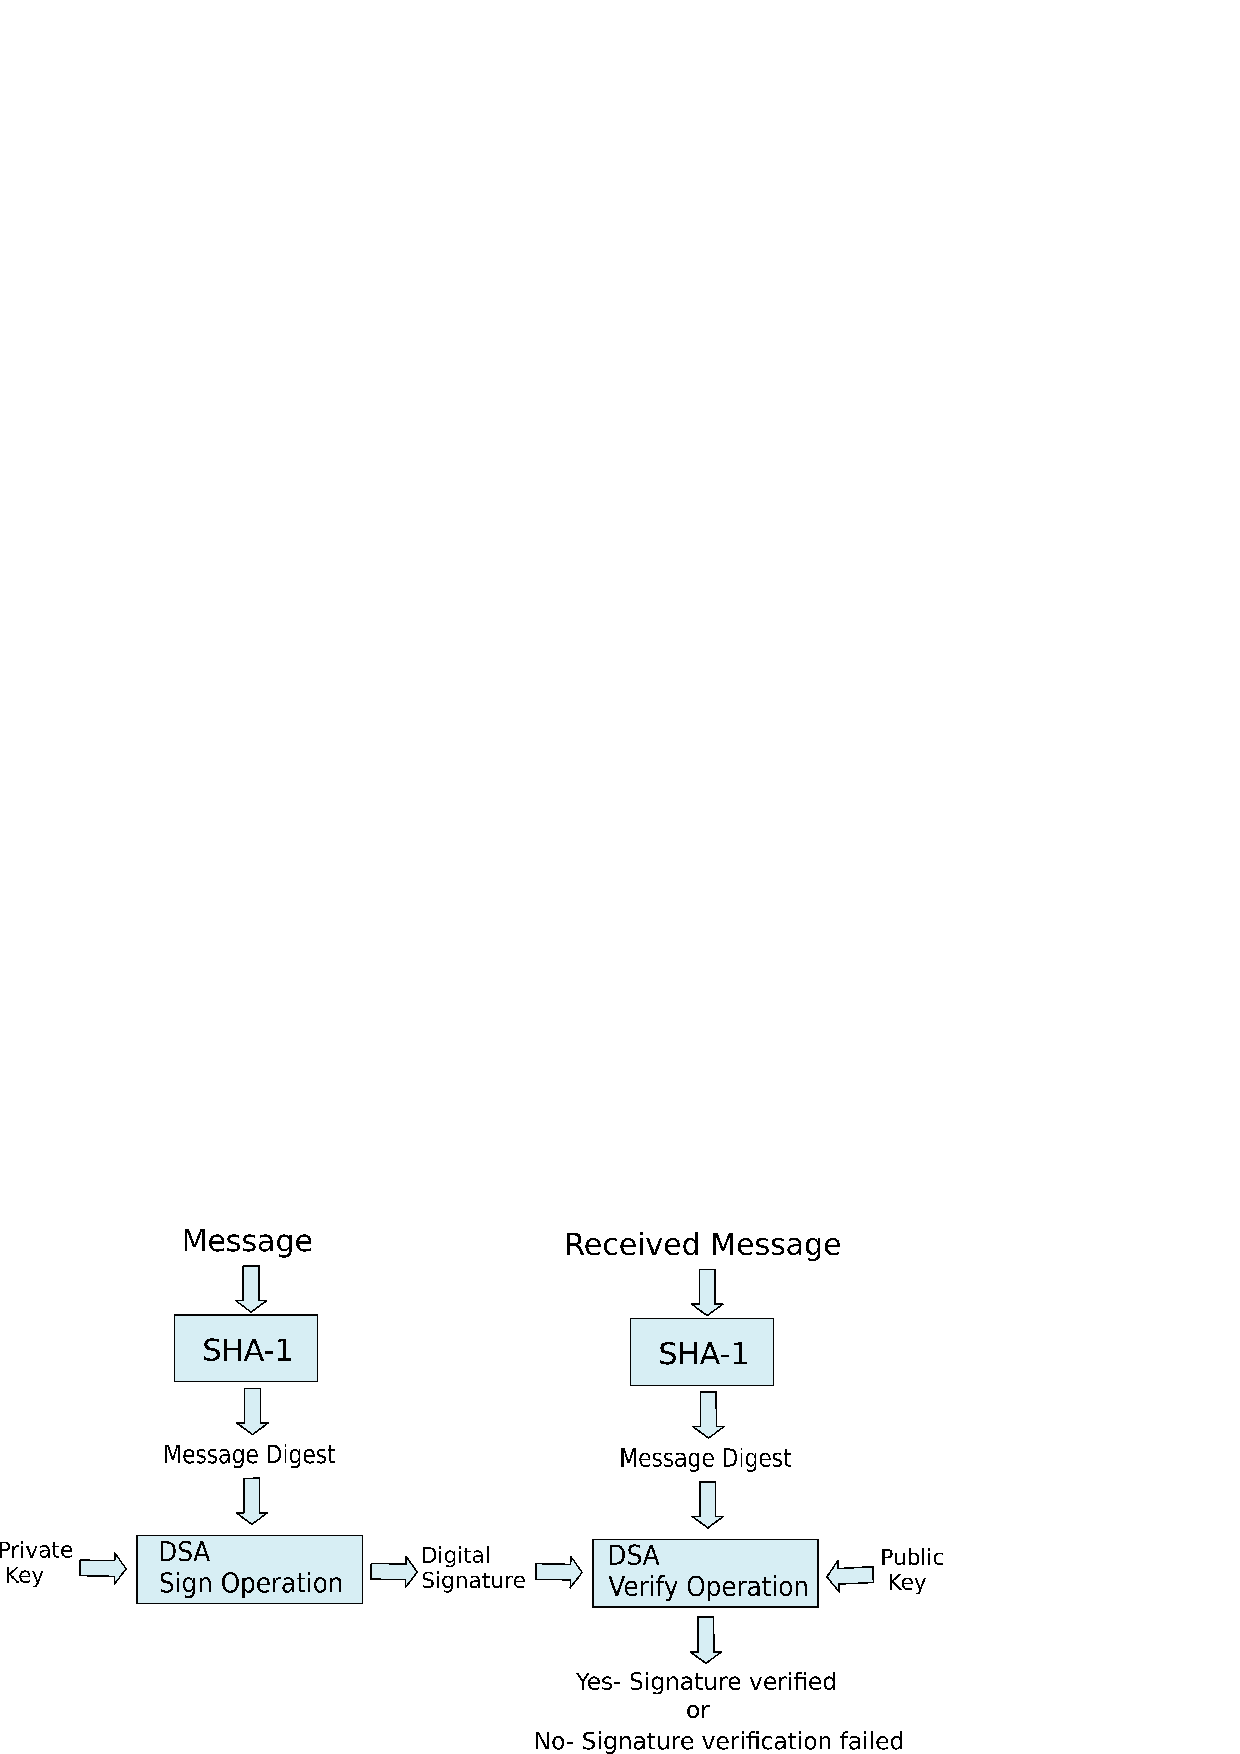
\includegraphics[scale=0.7]{Pictures/DSA_En_De.pdf} 
\caption{Workflow of the DSA algorithm. Adapted from \cite{DSA-FIPS}.}\label{StructureDSA}
\end{figure}
\subsubsection*{Types}
\begin{lstlisting}{}
  subtype DSA_Number is Bytes(0..Size/8-1);
  type Public_Key_DSA  is private;
  type Private_Key_DSA is private;
  type Signature_DSA   is private;
\end{lstlisting}
The \texttt{DSA\_Number} is a byte array which interprets a number. Its first element ($'First$) corresponds the most significant byte and the last element ($'Last$) corresponds the least significant byte of the number.\\
As required in DSA, each key has four parameters:
\begin{lstlisting}{}
  type DSA_KEY is record
      P : Big_Unsigned;
      Q : Big_Unsigned;
      G : Big_Unsigned;
      K : Big_Unsigned; 
  end record;
  type Public_Key_DSA is new DSA_KEY;
  type Private_Key_DSA is new DSA_KEY;
\end{lstlisting}\\
\subsubsection*{Procedures}
\begin{lstlisting}{}
  procedure Gen_Key(Public_Key  : out Public_Key_DSA;
                    Private_Key : out Private_Key_DSA);
\end{lstlisting}
This procedure generates a pair of keys, which are a public key (\texttt{Public\_Key}) and a private key (\texttt{Private\_Key}).\\
\textbf{Exception:} If the value $P$ of the public key is less than 3:\quad\texttt{Constraint\_Error}.\\
\hline \\ \ \\
\begin{lstlisting}{}
  procedure Sign(Private_Key : in  Private_Key_DSA;
                 SHA1_Hash   : in  W_Block160;
                 Signature   : out Signature_DSA);
\end{lstlisting}
This procedure signs the SHA-1 hash value (\texttt{SHA1\_Hash}) of a message with a private key (\texttt{Private\_Key}).\\
\hline \\ \ \\
\begin{lstlisting}{}
  function Verify(Public_Key  : Public_Key_DSA;
                  SHA1_Hash   : W_Block160;
                  Signature   : Signature_DSA) return Boolean;
\end{lstlisting}
This function returns true if the signature can be verified with the public key (\texttt{Public\_Key}) to be a valid signature of the SHA-1 hash value (\texttt{SHA1\_Hash}). If not, then false is returned.\\
With the public key only the signature created from the related private key can be verified. If the two keys don't match together, then the function returns false.\\
But if Bob uses the identity card of Alice, then we can't make identification of Bob with the card, although the identity card of Alice is valid.\\
\hline \\ \ \\
\begin{lstlisting}{}
  procedure Sign_File(Filename    : in  String;
                      Private_Key : in  Private_Key_DSA;
                      Signature   : out Signature_DSA);
\end{lstlisting}
With this procedure we can sign a file (\texttt{Filename}) with the private key (\texttt{Private\_Key}).\\
\textbf{Exception:}
%If the data is larger than $2^{26}TB$ :\quad \texttt{SHA1\_Constraint\_Error},\\
%Reading error\quad\quad\quad\quad\quad\quad\quad\quad :\quad \texttt{File\_Open\_Error},\\
If the \texttt{Private\_Key} is not initialized:\quad \texttt{Invalid\_Private\_Key\_Error}.\\
\hline \\ \ \\
\begin{lstlisting}{}
  function Verify_File(Filename   : String;
                       Public_Key : Public_Key_DSA;
                       Signature  : Signature_DSA) 
                       return Boolean;
\end{lstlisting}
This function returns true if the signature can be verified with the public key (\texttt{Public\_Key}) to be a valid signature of the file (\texttt{Filename}). If not, false is returned.\\
With the public key only the signature created from the related private key can be verified. If the two keys don't match together, then the function returns false.\\
\textbf{Exception:}
%If the data is larger than $2^{26}TB$ :\quad %\texttt{SHA1\_Constraint\_Error},\\
%Reading error\quad\quad\quad\quad\quad\quad\quad\quad :\quad \texttt{File\_Open\_Error},\\
If the \texttt{Public\_Key} is not initialized :\quad \texttt{Invalid\_Public\_Key\_Error}.\\
\hline \\ \ \\
\begin{lstlisting}{}
  function Verify_Key_Pair(Private_Key : Private_Key_DSA;
                           Public_Key  : Public_Key_DSA) 
                           return Boolean;
\end{lstlisting}
This function returns true if the two keys \texttt{Private\_Key} and \texttt{Public\_Key} match to each other, that is, they are a pair, if not, then false is returned.\\
\hline \\ \ \\
\begin{lstlisting}{}
  procedure Get_Public_Key(Public_Key : in Public_Key_DSA;
                           P          : out DSA_Number;
                           Q          : out DSA_Number;
                           G          : out DSA_Number;
                           Y          : out DSA_Number);
\end{lstlisting}
This procedure decomposes a public key (\texttt{Public\_Key}) into four components:
\begin{itemize}
\item One size-bit prime number $P$
\item One 160 bit prime number $Q$
\item One generator $G$ which $G=H^{(P-1)/Q}\mod P,\quad 1<H<P-1$
\item The real public key $Y$
\end{itemize}
With the four components the public key can be reconstructed later.\\
\hline \\ \ \\
\begin{lstlisting}{}
  procedure Get_Private_Key(Private_Key : in Private_Key_DSA;
                            P           : out DSA_Number;
                            Q           : out DSA_Number;
                            G           : out DSA_Number;
                            X           : out DSA_Number);
\end{lstlisting}
The private key \texttt{Private\_Key} is decomposed into four components:
\begin{itemize}
\item One size-bit prime number $P$
\item One 160 bit prime number $Q$
\item One generator $G$ which $G=H^{(P-1)/Q}\mod P,\quad 1<H<P-1$
\item The real private key $X$
\end{itemize}
With the four components the private key can be reconstructed later.\\
\hline \\ \ \\
\begin{lstlisting}{}
  procedure Set_Public_Key(P          : in DSA_Number;
                           Q          : in DSA_Number;
                           G          : in DSA_Number;
                           Y          : in DSA_Number;
                           Public_Key : out Public_Key_DSA);
\end{lstlisting}
During this procedure a public key can be (re-)constructed. The following values are required:
\begin{itemize}
\item One size-bit prime number $P$
\item One 160 bit prime number $Q$
\item One generator $G$ which is a subgroup of $Z^*_P$ with order $Q$
\item The real public key $Y$
\end{itemize}
\textbf{Exception:}\\ If any of the following conditions is met, then the \texttt{Invalid\_Public\_Key\_Error} is raised:\\
1) the length of $P$ is not equal the \texttt{Size}\,,\\
2) the length of $Q$ is not 160 bits\,, \\
3) the term $G$ is not in the range: $1<G<P$\,,\\
4) the term $Y$ is equal zero\,.\\
\hline \\ \ \\
\begin{lstlisting}{}
  procedure Set_Private_Key(P           : in DSA_Number;
                            Q           : in DSA_Number;
                            G           : in DSA_Number;
                            X           : in DSA_Number;
                            Private_Key : out Private_Key_DSA);
\end{lstlisting}
A private key can be (re-)constructed. The following values are required:
\begin{itemize}
\item One size-bit prime number $P$
\item One 160-bit prime number $Q$
\item One generator $G$ which is a subgroup of $Z^*_P$ with order $Q$
\item The real private key $X$
\end{itemize}
\textbf{Exception:}\\ If any of the following conditions is met, then the \texttt{Invalid\_Private\_Key\_Error} is raised:\\
1) the length of $P$ is not equal the \texttt{Size}\,,\\
2) the length of $Q$ is not 160 bits\,, \\
3) the term $G$ is not in the range: $1<G<P$\,,\\
4) the term $X$ is equal zero\,.
\section{Example}
\begin{lstlisting}{}
  with Ada.Text_IO;
  with Crypto.Types.Big_Numbers;
  with Crypto.Asymmetric.DSA;
  use Ada.Text_IO;
  procedure Example_DSA is
    package DSA is new Crypto.Asymmetric.DSA(512);
    use DSA;
    Public_Key : Public_Key_DSA;
    Private_Key : Private_Key_DSA;
    Signature : Signature_DSA;
  begin
    -- Key Generation
    Gen_Key(Public_Key, Private_Key);
    Sign_File("Example_DSA.adb", Private_Key, Signature);
    -- Verification
    if Verify_File("Example_DSA.adb", Public_Key, Signature) then
        Put_Line("OK");
    else 
        Put_Line("Error");
    end if;
  end Example_DSA;
\end{lstlisting}
%  \chapter{Crypto.Asymmetric.RSA}
RSA is an algorithm for public-key cryptography that is based on the presumed difficulty of factoring large integers. RSA stands for Ron Rivest, Adi Shamir and Leonard Adleman, who first publicly described it in \cite{PKCS} in 1978. Plaintext(-blocks) or ciphertext(-blocks) are encrypted or decrypted in OAEP (Optimal Asymmetric Encryption Padding), which is recommended in PKCS1-v2-1 (Public-Key Cryptography Standards) \cite{PKCS}.
\subsubsection*{OEAP Details}
\begin{itemize}
\item The implementation uses SHA1 inside MGF (Mask Generation Function: a function generating an arbitrary number of bits for a given input)
\item The implementation doesn't support the optional label L, i.e. L is always an empty string.
\end{itemize}
\subsubsection*{Generic Part}
\begin{lstlisting}{}
  generic
    Size : Positive;
\end{lstlisting}
\textbf{Exception:} If Size $< 512$ :\quad \texttt{Constraint\_Size\_Error}.\\
\section{API}
\subsection*{Types}
\begin{lstlisting}{}
  subtype RSA_Number is Bytes(0..Size/8-1);
  type Public_Key_RSA is private;
  type Private_Key_RSA is private;
\end{lstlisting}
The \texttt{RSA\_Number} is a byte array which interprets a number. Its first element ($'First$) corresponds the most significant byte and the last element ($'Last$) corresponds the least significant byte of the array.\\
\begin{lstlisting}{}
  type Public_Key_RSA is record
    N : Big_Unsigned;
    E : Big_Unsigned;
  end record;
  type Private_Key_RSA is record
    N : Big_Unsigned;
    D : Big_Unsigned;
    Phi : Big_Unsigned;
  end record;
\end{lstlisting}
The term \texttt{Public\_Key\_RSA} has two components, and \texttt{Private\_Key\_RSA} has three components. They are used in internal functions to generate key pairs.\\
\subsubsection*{High-Level-API}
\begin{lstlisting}{}
  procedure Gen_Key(Public_Key  : out Public_Key_RSA;
                    Private_Key : out Private_Key_RSA);
\end{lstlisting}
This procedure generates randomly a pair of keys, which are a public key (\texttt{Public\_Key}) and a private key (\texttt{Private\_Key}), by calculating all components of the key pair.\\
\begin{lstlisting}{}
  function Verify_Key_Pair(Private_Key : Private_Key_RSA;
                           Public_Key  : Public_Key_RSA) 
                           return Boolean;
\end{lstlisting}
This function returns true if the two keys, \texttt{Private\_Key} and \texttt{Public\_Key}, are a pair, if not, then false is returned.\\
\hline \\ \ \\
\begin{lstlisting}{}
  function OAEP_Encrypt(Public_Key : in  Public_Key_RSA;
                        Plaintext  : in  Bytes) 
                        return RSA_Number;
\end{lstlisting}
The function \texttt{OAEP\_Encrypt()} encrypts a plaintext(-block) (\texttt{Plaintext}) in the OEAP-Process and returns a ciphertext. 
The plaintext $M$ is encoded as a part of a data block $DB$, where the $lHash$ is a 160-bit hash value of an empty string. The data block $DB$ of length $k$ can be formed as:
\begin{equation*}
DB=lHash||PS||0\mbox{x}01||M\,,
\end{equation*}
where the string $PS$ consists of $k-160-8-|M|$ zero bits, its length may be zero, and 0x01 is a hexadecimal value. The data block is encoded (to a message $EM$) and encrypted to the ciphertext.
Detailed information about the \texttt{OAEP\_Encrypt()} can be found in \cite{PKCS}. The length limitation of the plaintext is defined as:
\texttt{Size/8}$-42\;(42=2*20+2)$.\\
\textbf{Exception:}\\
If the length of the plaintext is greater than the limitation:\quad \texttt{Plaintext\_Too\_Long\_Error};\\
\hline \\ \ \\
\begin{lstlisting}{}
  function OAEP_Decrypt(Private_Key : in  Private_Key_RSA;
                        Ciphertext  : in  RSA_Number) 
                        return Bytes;
\end{lstlisting}
This function decrypts a ciphertext(-block) (\texttt{Ciphertext}) under the private key. If the used private key and its related public key are a pair generated by \texttt{Gen\_Key()}, then the ciphertext is recovered to a data block as the structure shown in \texttt{OAEP\_Encrypt()}, and the plaintext is separated. Detailed information about the \texttt{OAEP\_Decrypt()} can be found in \cite{PKCS}.\\
\textbf{Exception:}\\
If one of the following conditions is met, then a  \texttt{Decrypt\_Error} is raised:\\
1) the ciphertext is greater than the RSA-Modulus $N$\,,\\
2) the first value of the $EM$ (\texttt{OAEP\_Encrypt()}) is not zero\,,\\
3) the term $lHash'$ of the new data block is not equal $lHash$ in \texttt{OAEP\_Encrypt()}.\\
\hline \\ \ \\
\begin{lstlisting}{}
  procedure Get_Public_Key(Public_Key : in Public_Key_RSA;
                           N          : out RSA_Number;
                           E          : out RSA_Number);
\end{lstlisting}
The procedure decomposes a public key (\texttt{Public\_Key}) into two components:
\begin{itemize}
\item One size-bit RSA modulus $N$ where $N=PQ$, where $P,Q$ are prime numbers
\item One public RSA exponent $E$
\end{itemize}
The public key can be reconstructed later with those two components.\\
\hline \\ \ \\
\begin{lstlisting}{}
  procedure Get_Private_Key(Private_Key : in Private_Key_RSA;
                            N           : out RSA_Number;
                            D           : out RSA_Number;
                            Phi         : out RSA_Number);
\end{lstlisting}
The procedure decomposes a private key (\texttt{Private\_Key}) into the following components:
\begin{itemize}
\item One size-bit RSA modulus $N$ where $N=PQ$, $P,Q$ are prime numbers
\item One private RSA exponent $D$
\item $\phi(N)=(P-1)(Q-1)$
\end{itemize}
The private key can be reconstructed later with those components.\\
\hline \\ \ \\
\begin{lstlisting}{}
  procedure Set_Public_Key(N          : in RSA_Number;
                           E          : in RSA_Number;
                           Public_Key : out Public_Key_RSA);
\end{lstlisting}
During the procedure a public key \texttt{Public\_Key} can be (re-)constructed. The following values are needed:
\begin{itemize}
\item One size-bit RSA modulus $N$
\item One public RSA exponent $E$
\end{itemize}
\textbf{Exception:}\\
If the public key is invalid, where the length of $N$ is not equal the \texttt{Size}, or the term $E$ is even or smaller than 3 :\quad \texttt{Constraint\_Error}.\\
\hline \\ \ \\
\begin{lstlisting}{}
  procedure Set_Private_Key(N           : in RSA_Number;
                            D           : in RSA_Number;
                            Phi         : in RSA_Number;
                            Private_Key : out Private_Key_RSA);
  procedure Set_Private_Key(N           : in Big_Unsigned;
                            D           : in Big_Unsigned;
                            Phi         : in Big_Unsigned;
                            Private_Key : out Private_Key_RSA);
\end{lstlisting}
The two procedures can both be used to (re-)construct a private key. The following values are required as parameters:
\begin{itemize}
\item One size-bit RSA modulus $N$ where $N=PQ$, $P,Q$ prime numbers
\item One private RSA exponent $D$
\item $\phi(N)=(P-1)(Q-1)$
\end{itemize}
\textbf{Exception:}\\ If one of the following conditions about the private key is met, then a \texttt{Constraint\_Error} is raised:\\
1) the length of $N$ is not equal the \texttt{Size}\,,\\
2) the term $D$ is even, or its bit value is smaller than or equal 2\,, \\
3) the term $\phi(N)$ is odd, or its length is smaller than \texttt{Size}-2\,,\\
4) the greatest common divisor of $D$ and $\phi(N)$ is not 1\,.
\subsubsection*{Low-Level-API}
The Low-Level-API can be used only when users know exactly what it does. Naive usage of the API can lead to critic security problems, cause identical plaintexts can be encrypted to identical ciphertexts.
\begin{lstlisting}{}
  procedure Encrypt(Public_Key : in  Public_Key_RSA;
                    Plaintext  : in  RSA_Number;
                    Ciphertext : out RSA_Number);   
  procedure Encrypt(Public_Key : in  Public_Key_RSA;
                    Plaintext  : in  Big_Unsigned;
                    Ciphertext : out Big_Unsigned);
\end{lstlisting}
The procedures encrypt a plaintext to a ciphertext with a public key. They use the "naive" RSA-Process ($C=P^{K.E}$(mod $K.N$)).\\
\textbf{Exception:}\\
If the public key is invalid, where the length of $N$ is not equal the \texttt{Size}, or the term $E$ is even or smaller than 3 :\quad \texttt{Invalid\_Public\_Key\_Error}.\\
\hline \\ \ \\
\begin{lstlisting}{}
  procedure Decrypt(Private_Key : in  Private_Key_RSA;
                    Ciphertext  : in  RSA_Number;
                    Plaintext   : out RSA_Number);
  procedure Decrypt(Private_Key : in  Private_Key_RSA;
                    Ciphertext  : in  Big_Unsigned;
                    Plaintext   : out Big_Unsigned);
\end{lstlisting}
The two procedures can be both used to decrypt a ciphertext. It checks at first if the private key is valid or not, and then it decrypts the ciphertext to a plaintext with the private key. They use the "naive" RSA-Process ($P=C^{K.D}$ (mod $K.N$)).\\
\textbf{Exception:}\\ If one of the following conditions about the private key is met, then a \texttt{Decrypt\_Error} is raised:\\
1) the length of $N$ is not equal the \texttt{Size}\,,\\
2) the term $D$ is even, or its bit value is smaller than or equal 2\,, \\
3) the term $\phi(N)$ is odd, or its length is smaller than \texttt{Size}-2\,,\\
4) the greatest common divisor of $D$ and $\phi(N)$ is not 1\,.
\section{Example}
\begin{lstlisting}{}
  with Crypto.Types; use Crypto.Types;
  with Crypto.Asymmetric.RSA;
  with Ada.Text_IO; use Ada.Text_IO;
  procedure Example_RSA is
    package RSA is new Crypto.Asymmetric.RSA(512);
    use RSA;
    Message : Bytes := To_Bytes("Good Luck!");
    Public_Key : Public_Key_RSA;
    Private_Key : Private_Key_RSA;
  begin
    Gen_Key(Public_Key, Private_Key); -- Generation of key pair
    declare 
      -- Encryption & Decryption
	  Ciphertext:RSA_Number:= OAEP_Encrypt(Public_Key, Message);
	  Plaintext:Bytes:= OAEP_Decrypt(Private_Key, Ciphertext);
    begin
      Put(To_String(Ciphertext)); -- Output of ciphertext
	   New_Line;
      Put(To_String(Plaintext)); -- Output of plaintext
    end;
  end Example_RSA;
\end{lstlisting}


%literature
\bibliographystyle{plain} 
\bibliography{crypto}

\end{document}

    
    


